\documentclass[12pt,letterpaper]{article}
\usepackage[utf8]{inputenc}
\usepackage[spanish]{babel}
\usepackage{graphicx}
\usepackage[hidelinks]{hyperref}
\usepackage{hyperref}
\usepackage[left=2cm,right=2cm,top=2.5cm,bottom=2cm]{geometry}
\usepackage{graphicx} % figuras
\usepackage{float} % para usar [H]
\usepackage{amsmath}
\usepackage{stackrel} 
\usepackage{multicol}
\usepackage{multirow}
\usepackage{fancyhdr}
\usepackage[usenames,dvipsnames,svgnames,table]{xcolor}
\usepackage[document]{ragged2e}
\usepackage{enumerate} % enumerados
\renewcommand{\labelitemi}{$-$}
\renewcommand{\labelitemii}{$\cdot$}
\newcommand\tab[1][1cm]{\hspace*{#1}}

\definecolor{amarillo}{RGB}{255,255,0}
\definecolor{rojo}{RGB}{255,0,0}
\definecolor{azul}{RGB}{0,0,255}
\definecolor{verdeClaro}{RGB}{0,255,0}

%encabezado
\pagestyle{fancy}
\lhead{\begin{picture}(0,0) \put(0,0){
\includegraphics[width=10mm]{./img/logo}} \end{picture}}
\chead{\hspace{1cm}\vspace{0.2cm}INFORME DE LABORATORIO N° 01 - VISUALIZACION DE DATOS CON TABLEAU}
\rhead{}

\begin{document}
    \begin{titlepage}
        \begin{center}
            \begin{figure}[htb]
                \begin{center}
                    
\includegraphics[width=3.5cm]{./img/logo}
                \end{center}
            \end{figure}
            \vspace*{0.15in}
            \begin{Large}
                \textbf{UNIVERSIDAD PRIVADA DE TACNA}\\
            \end{Large}
            \vspace*{0.15in}
            \begin{Large}
                \textbf{FACULTAD DE INGENIERIA} \\
            \end{Large}
            \vspace*{0.1in}
            \begin{Large}
                \textbf{Escuela Profesional de Ingeniería de Sistemas} \\
            \end{Large}
            \vspace*{0.3in}
            \begin{Large}
                \textbf{INFORME DE LABORATORIO N°01}\\
                \textbf{“VISUALIZACION DE DATOS CON TABLEAU}\\
            \end{Large}
            \vspace*{0.2in}
            \begin{Large}
                \textbf{CURSO:} \\
            \end{Large}
            \vspace*{0.1in}
            \begin{large}
                Inteligencia de Negocios\\
            \end{large}
            \vspace*{0.2in}
            \begin{Large}
                \textbf{DOCENTE:} \\
            \end{Large}
            \vspace*{0.1in}
            \begin{large}
                Mag. Patrick Jose Cuadros Quiroga\\
            \end{large}
            \vspace*{0.3in}
            \begin{large}
                \textbf{ALUMNO:} \\
                \begin{flushleft}
                    Gutierrez Ponce, José Carlos  		\hfill	(2017059277) \\
                \end{flushleft}
            \end{large}
            \vspace*{1.3in}
            \begin{large}
                Tacna - Perú\\
            \end{large}
            \vspace*{0.1in}
            \begin{large}
                2021\\
            \end{large}
        \end{center}
    \end{titlepage}
    \include{Secciones/articulo}
    %%%%%%%%%%%%%%%%%%%%%%%%%%%%%%%%%%%%%%%%%%%%%%%%%%%%%%%%%%%%%%%%%%%%%%%%%%%%%%%%%%%%%%%%%%%%%%%%%%%%%%%%%%%%%%%%%%%%%%%%%%%%%%%%%%%%%%%%%%%%%%%%%%%%%%%%%%%%%%%%%%%%%%%%%%%%%%%%%%%%%%%%%%%%%%%%%%%%%%%%%%%%%%%%%%%%%%%%%%%%%%%%%%%%%%%%%%%%%%%%%%%%%%%%%%%%%%%%%%%%%%%%%%%%%%%%%%%%%%%%%%%%%%%%%%%%%%%%%%%%%%%%%%%%%%%%%%%%%%%%%%%%%%%%%%%%%%%%%%%%%%%%%%%%%%%%%%%%%%%%%%%%%%%%%%%%%%%%%%%%%%%%%%%%%%%%%%%%%%%%%%%%%%%%%%%%%%%%%%%%%%%%%%%%%%%%%%%%%%%%%%%%%%%%%%%%%%%%%%%%%%%%%%%%%%%%%%%%%%%%%%%%%%%%%%%%%%%
    \newpage
    \tableofcontents
    \justify
    %%%%%%%%%%%%%%%%%%%%%%%%%%%%%%%%%%%%%%%%%%%%%%%%%%%%%%%%%%%%%%%%%%%%%%%%%%%%%%%%%%%%%%%%%%%%%%%%%%%%%%%%%%%%%%%%%%%%%%%%%%%%%%%%%%%%%%%%%%%%%%%%%%%%%%%%%%%%%%%%%%%%%%%%%%%%%%%%%%%%%%%%%%%%%%%%%%%%%%%%%%%%%%%%%%%%%%%%%%%%%%%%%%%%%%%%%%%%%%%%%%%%%%%%%%%%%%%%%%%%%%%%%%%%%%%%%%%%%%%%%%%%%%%%%%%%%%%%%%%%%%%%%%%%%%%%%%%%%%%%%%%%%%%%%%%%%%%%%%%%%%%%%%%%%%%%%%%%%%%%%%%%%%%%%%%%%%%%%%%%%%%%%%%%%%%%%%%%%%%%%%%%%%%%%%%%%%%%%%%%%%%%%%%%%%%%%%%%%%%%%%%%%%%%%%%%%%%%%%%%%%%%%%%%%%%%%%%%%%%%%%%%%%%%%%%%%%%
    \newpage
    \begin{LARGE}
        \begin{center}
            \textbf{VISUALIZACION DE DATOS CON TABLEAU} \\
        \end{center}
    \end{LARGE}
    %%%%%%%%%%%%%%%%%%%%%%%%%%%%%%%%%%%%%%%%%%%%%%%%%%%%%%%%%%%%%%%%%%%%%%%%%%%%%%%%%%%%%%%%%%%%%%%%%%%%%%%%%%%%%%%%%%%%%%%%%%%%%%%%%%%%%%%%%%%%%%%%%%%%%%%%%%%%%%%%%%%%%%%%%%%%%%%%%%%%%%%%%%%%%%%%%%%%%%%%%%%%%%%%%%%%%%%%%%%%%%%%%%%%%%%%%%%%%%%%%%%%%%%%%%%%%%%%%%%%%%%%%%%%%%%%%%%%%%%%%%%%%%%%%%%%%%%%%%%%%%%%%%%%%%%%%%%%%%%%%%%%%%%%%%%%%%%%%%%%%%%%%%%%%%%%%%%%%%%%%%%%%%%%%%%%%%%%%%%%%%%%%%%%%%%%%%%%%%%%%%%%%%%%%%%%%%%%%%%%%%%%%%%%%%%%%%%%%%%%%%%%%%%%%%%%%%%%%%%%%%%%%%%%%%%%%%%%%%%%%%%%%%%%%%%%%%%
    \section{OBJETIVOS}
    \begin{itemize}
        \item Comprender la organización la información de nuestros datos de tal manera que todos los que los vean puedan comprender sus implicaciones y cómo actuar sobre ellos con claridad.
    \end{itemize}
    %%%%%%%%%%%%%%%%%%%%%%%%%%%%%%%%%%%%%%%%%%%%%%%%%%%%%%%%%%%%%%%%%%%%%%%%%%%%%%%%%%%%%%%%%%%%%%%%%%%%%%%%%%%%%%%%%%%%%%%%%%%%%%%%%%%%%%%%%%%%%%%%%%%%%%%%%%%%%%%%%%%%%%%%%%%%%%%%%%%%%%%%%%%%%%%%%%%%%%%%%%%%%%%%%%%%%%%%%%%%%%%%%%%%%%%%%%%%%%%%%%%%%%%%%%%%%%%%%%%%%%%%%%%%%%%%%%%%%%%%%%%%%%%%%%%%%%%%%%%%%%%%%%%%%%%%%%%%%%%%%%%%%%%%%%%%%%%%%%%%%%%%%%%%%%%%%%%%%%%%%%%%%%%%%%%%%%%%%%%%%%%%%%%%%%%%%%%%%%%%%%%%%%%%%%%%%%%%%%%%%%%%%%%%%%%%%%%%%%%%%%%%%%%%%%%%%%%%%%%%%%%%%%%%%%%%%%%%%%%%%%%%%%%%%%%%%%%
    \section{REQUERIMIENTOS}
    \begin{itemize}
        \item Conocimientos\\
        Para el desarrollo de esta práctica se requerirá de los siguientes conocimientos básicos:
        \begin{itemize} 
            \item Conocimientos básicos en el uso de Qlik Sense.
        \end{itemize}
        \item Hardware
        \begin{itemize}
            \item CPU SLAT-capable feature.
            \item Al menos 4GB de RAM.
        \end{itemize}
        \item Software\\
        Así mismo se necesitan los siguientes aplicativos
        \begin{itemize}
            \item Windows 10 64bit: Pro, Enterprise o Education (1607 Anniversary Update, Build 14393 o Superior) 
            \item Tableau Desktop, 64 bits descargable desde (\textcolor{azul}{\url{https://downloads.tableau.com/tssoftwareregistered/TableauDesktop-64bit-2021-1-0.exe}}).
        \end{itemize}
    \end{itemize}
    %%%%%%%%%%%%%%%%%%%%%%%%%%%%%%%%%%%%%%%%%%%%%%%%%%%%%%%%%%%%%%%%%%%%%%%%%%%%%%%%%%%%%%%%%%%%%%%%%%%%%%%%%%%%%%%%%%%%%%%%%%%%%%%%%%%%%%%%%%%%%%%%%%%%%%%%%%%%%%%%%%%%%%%%%%%%%%%%%%%%%%%%%%%%%%%%%%%%%%%%%%%%%%%%%%%%%%%%%%%%%%%%%%%%%%%%%%%%%%%%%%%%%%%%%%%%%%%%%%%%%%%%%%%%%%%%%%%%%%%%%%%%%%%%%%%%%%%%%%%%%%%%%%%%%%%%%%%%%%%%%%%%%%%%%%%%%%%%%%%%%%%%%%%%%%%%%%%%%%%%%%%%%%%%%%%%%%%%%%%%%%%%%%%%%%%%%%%%%%%%%%%%%%%%%%%%%%%%%%%%%%%%%%%%%%%%%%%%%%%%%%%%%%%%%%%%%%%%%%%%%%%%%%%%%%%%%%%%%%%%%%%%%%%%%%%%%%%
    \section{CONSIDERACIONES INICIALES}
    \begin{itemize}
        \item Tener licencia de estudiante en Tableau (\textcolor{azul}{https://www.tableau.com/academic/students}).
        \item Tener el archivo ExerciseData.xlsx, se puede descargar desde \textcolor{azul}{\href{https://learning.qlik.com/mod/resource/view.php?id=22519}{aca}}
    \end{itemize}
    %%%%%%%%%%%%%%%%%%%%%%%%%%%%%%%%%%%%%%%%%%%%%%%%%%%%%%%%%%%%%%%%%%%%%%%%%%%%%%%%%%%%%%%%%%%%%%%%%%%%%%%%%%%%%%%%%%%%%%%%%%%%%%%%%%%%%%%%%%%%%%%%%%%%%%%%%%%%%%%%%%%%%%%%%%%%%%%%%%%%%%%%%%%%%%%%%%%%%%%%%%%%%%%%%%%%%%%%%%%%%%%%%%%%%%%%%%%%%%%%%%%%%%%%%%%%%%%%%%%%%%%%%%%%%%%%%%%%%%%%%%%%%%%%%%%%%%%%%%%%%%%%%%%%%%%%%%%%%%%%%%%%%%%%%%%%%%%%%%%%%%%%%%%%%%%%%%%%%%%%%%%%%%%%%%%%%%%%%%%%%%%%%%%%%%%%%%%%%%%%%%%%%%%%%%%%%%%%%%%%%%%%%%%%%%%%%%%%%%%%%%%%%%%%%%%%%%%%%%%%%%%%%%%%%%%%%%%%%%%%%%%%%%%%%%%%%%%
    \newpage
    \section{DESARROLLO}
    %%%%%%%%%%%%%%%%%%%%%%%%%%%%%%%%%%%%%%%%%%%%%%%%%%%%%%%%%%%%%%%%%%%%%%%%%%%%%%%%%%%%%%%%%%%%%%%%%%%%%%%%%%%%%%%%%%%%%%%%%%%%%%%%%%%%%%%%%%%%%%%%%%%%%%%%%%%%%%%%%%%%%%%%%%%%%%%%%%%%%%%%%%%%%%%%%%%%%%%%%%%%%%%%%%%%%%%%%%%%%%%%%%%%%%%%%%%%%%%%%%%%%%%%%%%%%%%%%%%%%%%%%%%%%%%%%%%%%%%%%%%%%%%%%%%%%%%%%%%%%%%%%%%%%%%%%%%%%%%%%%%%%%%%%%%%%%%%%%%%%%%%%%%%%%%%%%%%%%%%%%%%%%%%%%%%%%%%%%%%%%%%%%%%%%%%%%%%%%%%%%%%%%%%%%%%%%%%%%%%%%%%%%%%%%%%%%%%%%%%%%%%%%%%%%%%%%%%%%%%%%%%%%%%%%%%%%%%%%%%%%%%%%%%%%%%%%%
    \subsection{Introducción a Tableau}
    \paragraph{\Large Instalación\\ \\}
    Dependiendo de la elección del producto, descargue el software en la computadora. Después de aceptar el acuerdo de licencia, puede verificar la instalación haciendo clic en el ícono de Tableau. Si aparece la siguiente pantalla, está listo para comenzar.
    \begin{center}
        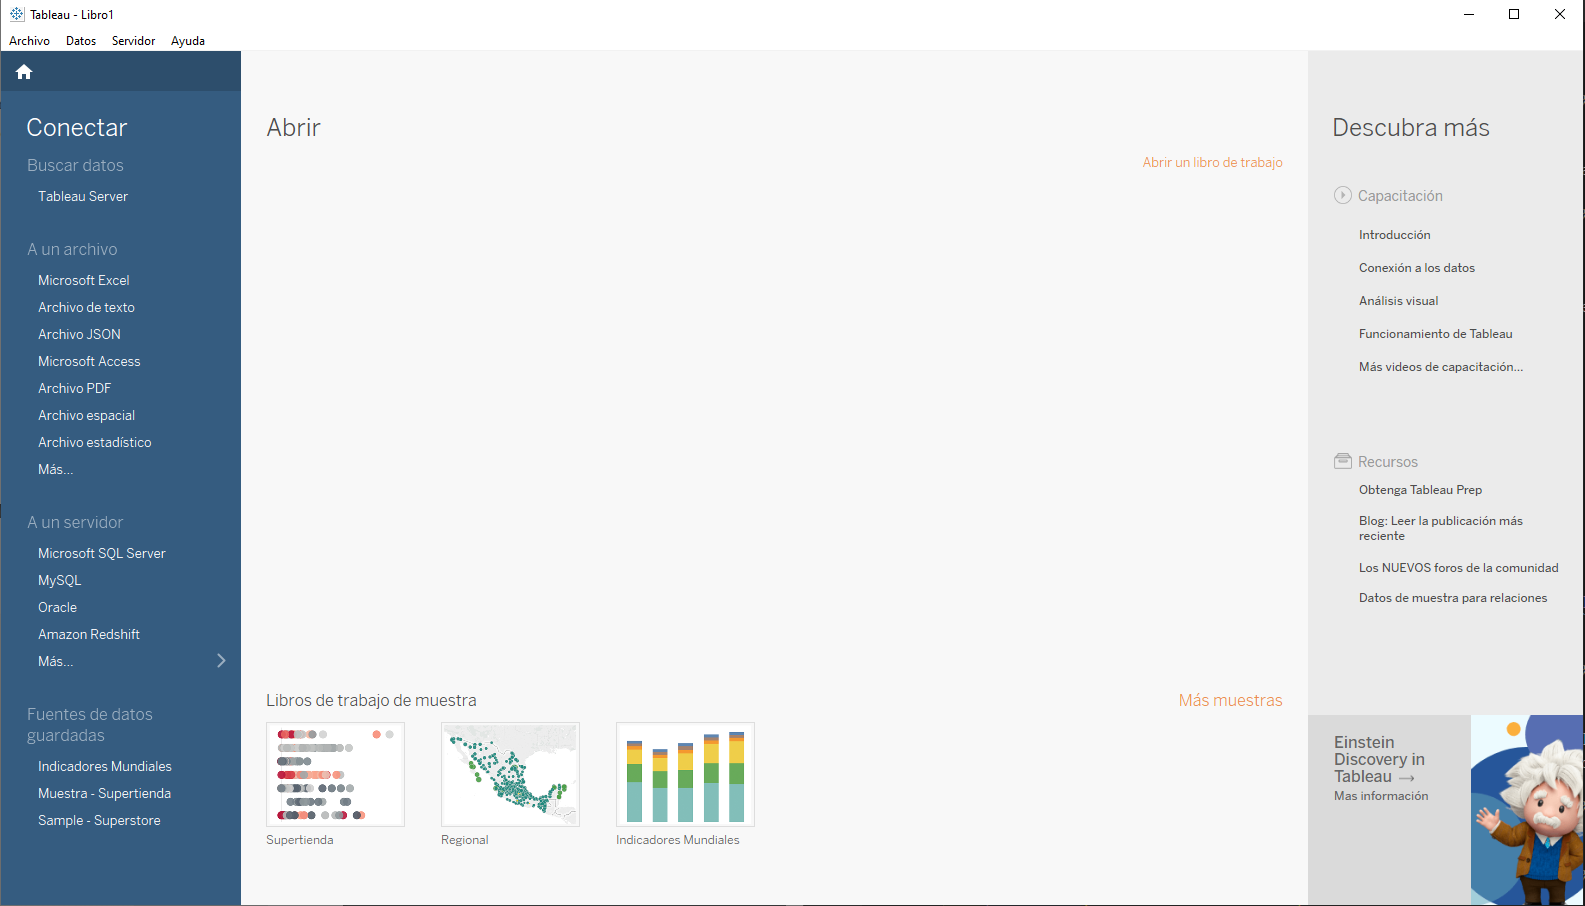
\includegraphics[width=16cm]{./img/img1.png}
    \end{center}
    %%%%%%%%%%%%%%%%%%%%%%%%%%%%%%%%%%%%%%%%%%%%%%%%%%%%%%%%%%%%%%%%%%%%%%%%%%%%%%%%%%%%%%%%%%%%%%%%%%%%%%%%%%%%%%%%%%%%%%%%%%%%%%%%%%%%%%%%%%%%%%%%%%%%%%%%%%%%%%%%%%%%%%%%%%%%%%%%%%%%%%%%%%%%%%%%%%%%%%%%%%%%%%%%%%%%%%%%%%%%%%%%%%%%%%%%%%%%%%%%%%%%%%%%%%%%%%%%%%%%%%%%%%%%%%%%%%%%%%%%%%%%%%%%%%%%%%%%%%%%%%%%%%%%%%%%%%%%%%%%%%%%%%%%%%%%%%%%%%%%%%%%%%%%%%%%%%%%%%%%%%%%%%%%%%%%%%%%%%%%%%%%%%%%%%%%%%%%%%%%%%%%%%%%%%%%%%%%%%%%%%%%%%%%%%%%%%%%%%%%%%%%%%%%%%%%%%%%%%%%%%%%%%%%%%%%%%%%%%%%%%%%%%%%%%%%%%%
    \subsection{Comenzar}
    En esta sección, aprenderemos algunas operaciones básicas en Tableau para acostumbrarnos a su interfaz.
    \paragraph{\Large Espacio de trabajo de Tableau \\ \\}
    El espacio de trabajo de Tableau es una colección de hojas de trabajo, barra de menú, barra de herramientas, tarjeta de marcas, estantes y muchos otros elementos sobre los que aprenderemos en las próximas secciones. Las hojas pueden ser hojas de trabajo, paneles o historias. La siguiente imagen destaca los componentes principales del espacio de trabajo. Sin embargo, se logrará una mayor familiaridad una vez que trabajemos con datos reales.
    \begin{center}
        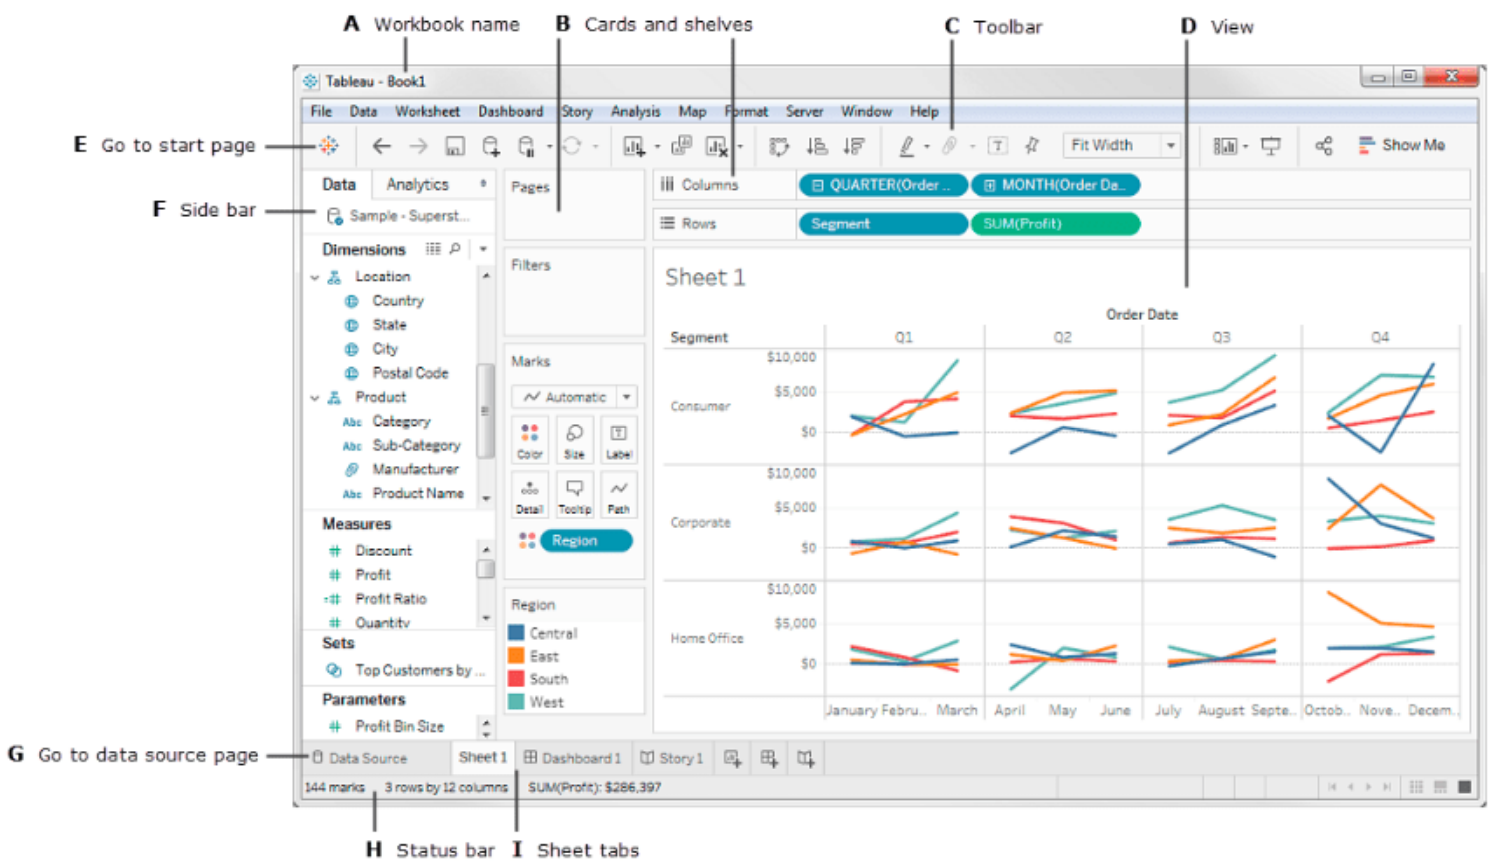
\includegraphics[width=16cm]{./img/img2.png}
    \end{center}
    %--------------------------------------------------------------------------------------------------------------------------------------------------------------------------------------------------------------------------------------------------------------------------------------------------------------------------------------------------------------------------------------------------------------------------------------------------------------------------------------------------------------
    \paragraph{\Large Conexión a una fuente de datos\\ \\}
    Para comenzar a trabajar con Tableau, debemos conectar Tableau a la fuente de datos. Tableau es compatible con muchas fuentes de datos. Las fuentes de datos compatibles con Tableau aparecen en el lado izquierdo de la pantalla inicial. Algunas fuentes de datos de uso común son Excel, archivos de texto, bases de datos relacionales o incluso en un servidor. También se puede conectar a una fuente de base de datos en la nube como Google Analytics, Amazon Redshift, etc.\\ \\
    La pantalla de inicio de Tableau Desktop muestra las fuentes de datos disponibles que también se pueden conectar. También depende de la versión de Tableau, ya que la versión de pago ofrece más posibilidades. En el lado izquierdo de la pantalla, hay un Connectpanel que resalta las fuentes disponibles. Los tipos de archivo se enumeran primero, seguidos de los tipos de servidor comunes o los servidores que se han conectado recientemente. Puede abrir libros de trabajo creados previamente en la Openpestaña Bajo . Tableau Desktop también proporciona algunos libros de trabajo de muestra a continuación \textit{Sample Workbooks}.
    \begin{center}
        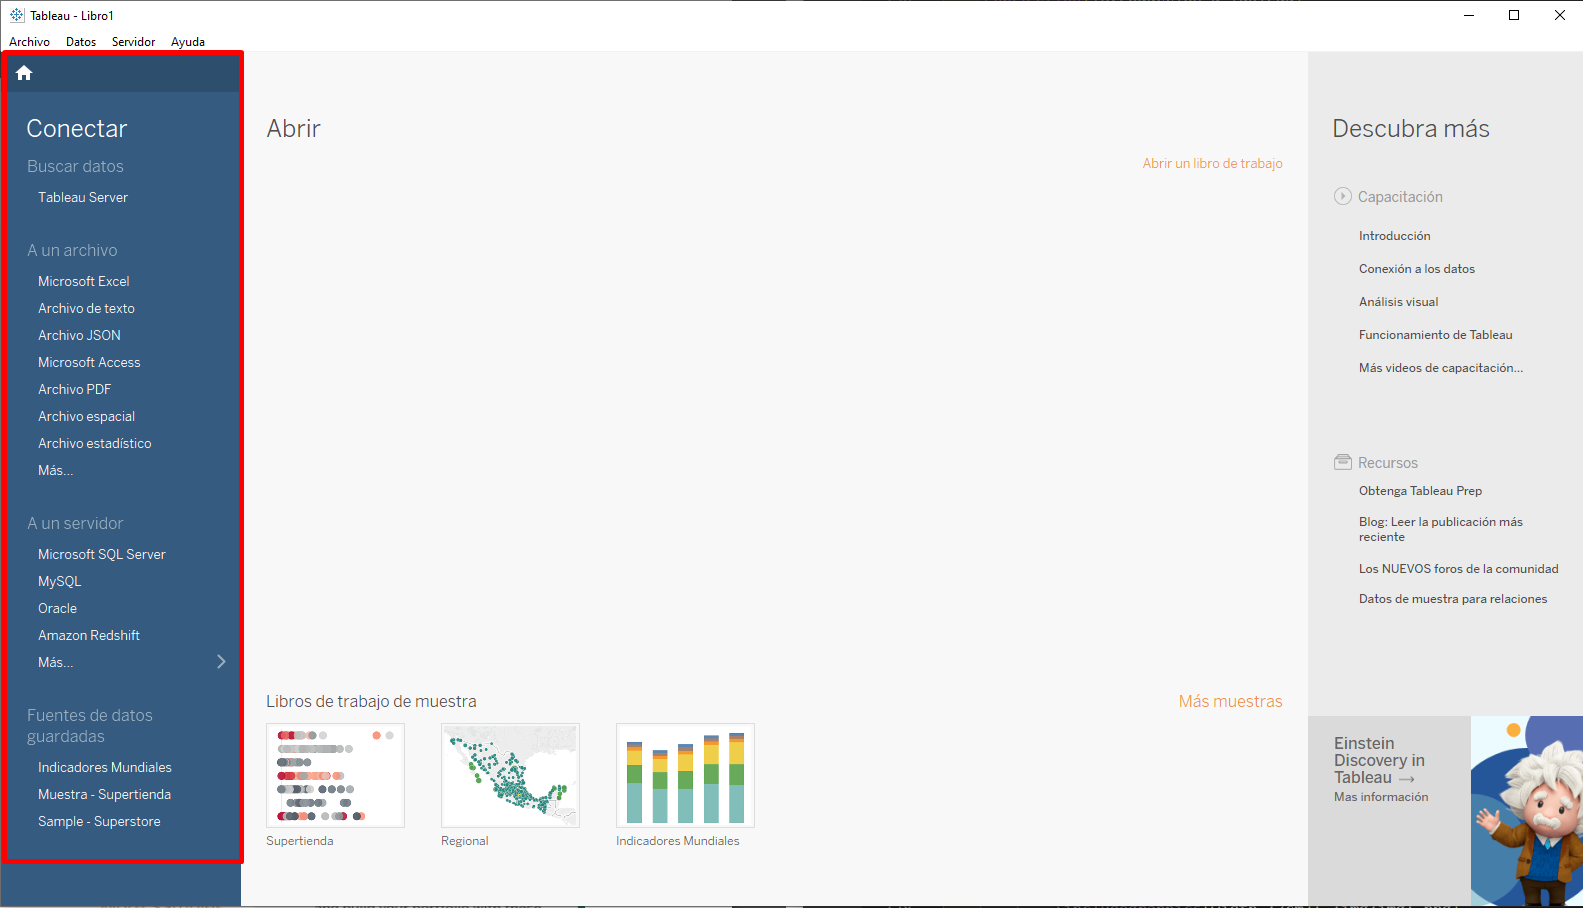
\includegraphics[width=16cm]{./img/img3.png}
    \end{center}
    Trabajaremos con un conjunto de datos de muestra con nombres Superstore dataset , que viene precargado con Tableau. Sin embargo, descargaremos el archivo desde aquí para que podamos tener una idea de cómo conectarnos a una fuente de datos de Excel. Los datos son los de un hipermercado. Contiene información sobre productos, ventas, beneficios, etc. Nuestro objetivo como analistas de datos es analizar los datos y encontrar áreas críticas de mejora dentro de esta empresa ficticia.
    \begin{enumerate}
        \item Importe los datos al espacio de trabajo de Tableau desde la computadora.
        \begin{center}
            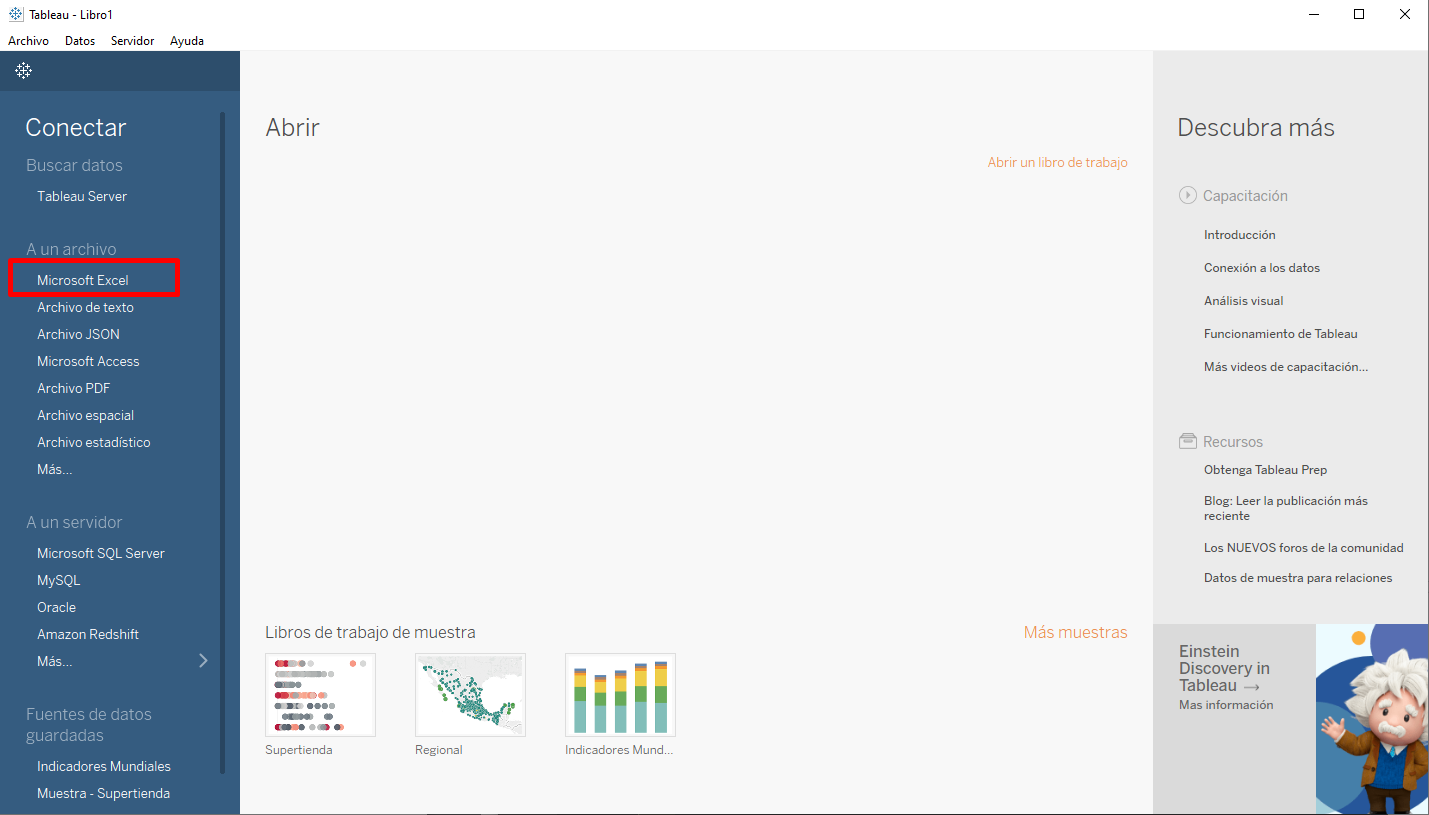
\includegraphics[width=15cm]{./img/img4.png}
        \end{center}
        \item Se nos cargara los datos del archivo seleccionado.
        \begin{center}
            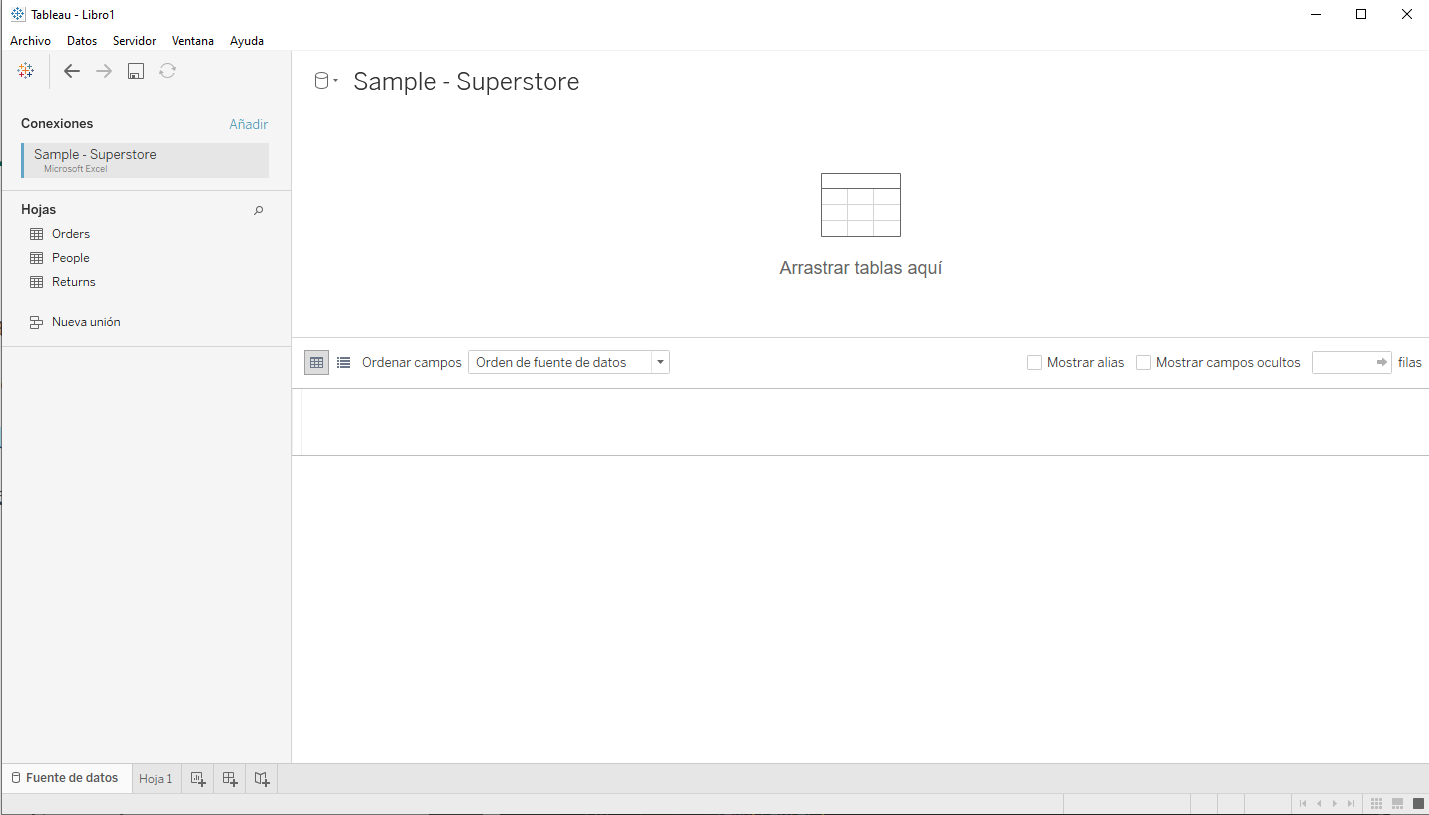
\includegraphics[width=15cm]{./img/img4.1.png}
        \end{center}
        \item En la pestaña Hojas, se verán tres hojas: \textbf{Pedidos}, \textbf{Personas} y \textbf{Devoluciones}.
        \begin{center}
            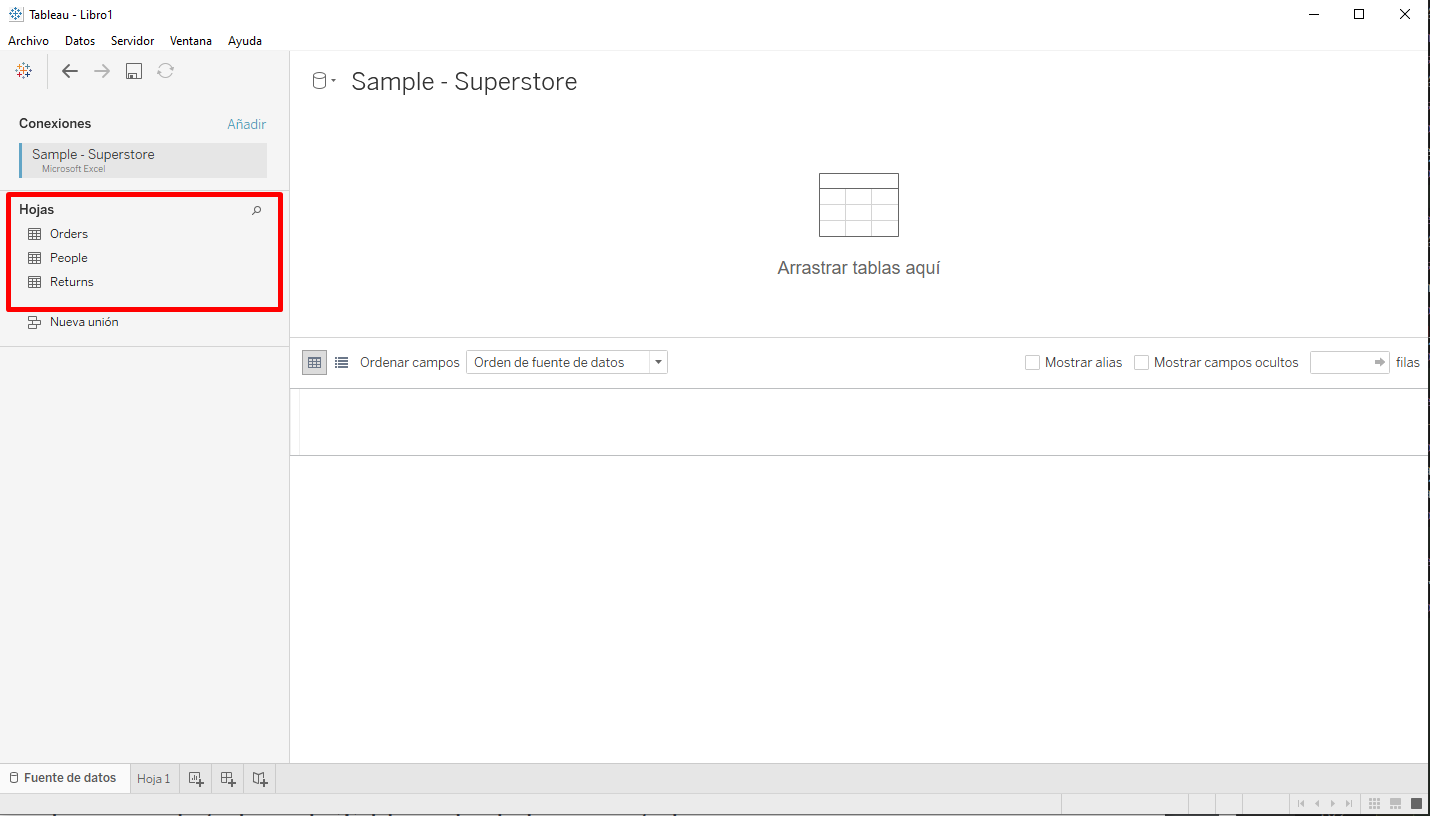
\includegraphics[width=15cm]{./img/img5.png}
        \end{center}
        \item Nos centraremos solo en los datos de los pedidos. Haga doble clic en Hoja de \textbf{pedidos} y se abrirá como una hoja de cálculo.
        \begin{center}
            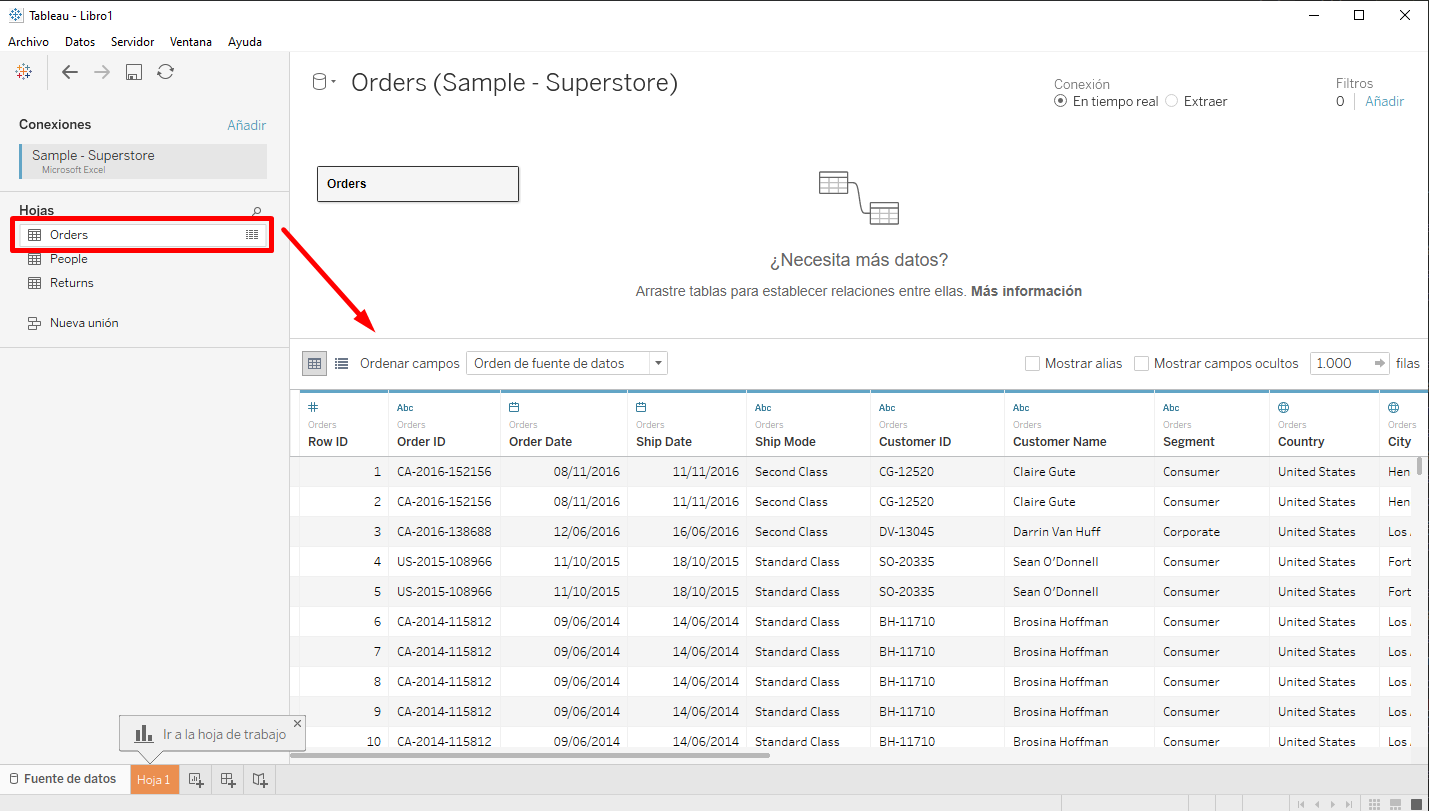
\includegraphics[width=15cm]{./img/img6.png}
        \end{center}
        \item Observamos que las primeras tres filas de datos se ven un poco diferentes y no están en el formato deseado.
        \begin{center}
            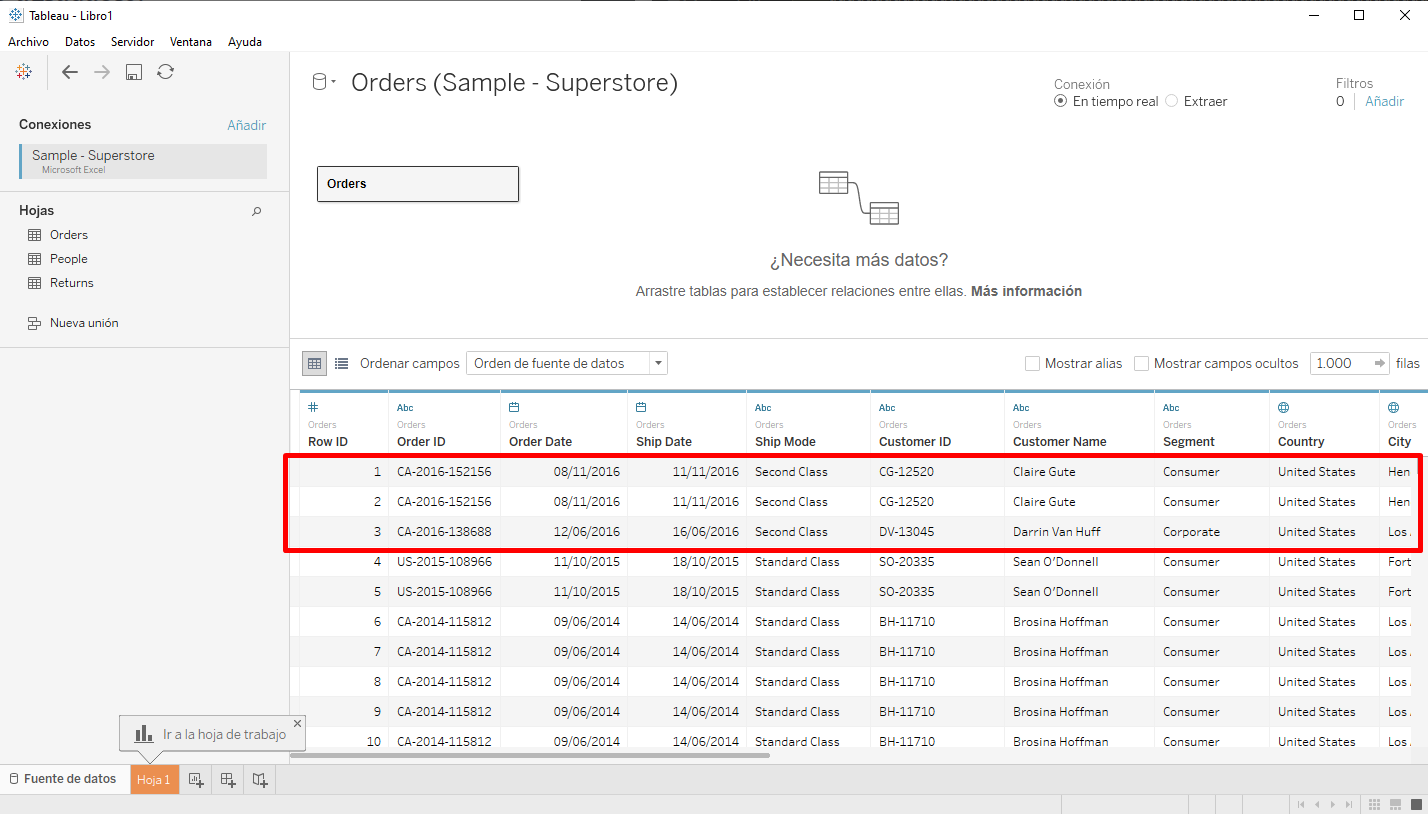
\includegraphics[width=15cm]{./img/img7.png}
        \end{center}
    \end{enumerate}
    %--------------------------------------------------------------------------------------------------------------------------------------------------------------------------------------------------------------------------------------------------------------------------------------------------------------------------------------------------------------------------------------------------------------------------------------------------------------------------------------------------------------
    \paragraph{\Large Crear una vista\\ \\}
    Comenzaremos generando un gráfico simple. En esta sección, conoceremos nuestros datos y comenzaremos a hacer preguntas sobre los datos para obtener información. Hay algunos términos importantes que encontraremos en esta sección
    \begin{itemize}
        \item \textbf{Las dimensiones:} Son datos cualitativos, como un nombre o una fecha. De forma predeterminada, Tableau clasifica automáticamente los datos que contienen información cualitativa o categórica como una dimensión, por ejemplo, cualquier campo con texto o valores de fecha. Estos campos generalmente aparecen como encabezados de columna para filas de datos, como Nombre del cliente o Fecha del pedido, y también definen el nivel de granularidad que se muestra en la vista.
        \item \textbf{Las medidas:} Son datos numéricos cuantitativos. De forma predeterminada, Tableau trata cualquier campo que contenga este tipo de datos como una medida, por ejemplo, transacciones de ventas o ganancias. Los datos que se clasifican como una medida se pueden agregar en función de una dimensión determinada, por ejemplo, las ventas totales (medida) por región (dimensión).
        \item \textbf{La agregacion:} Son los datos a nivel de fila acumulados en una categoría superior, como la suma de las ventas o el beneficio total.
    \end{itemize}
    Tableau ordena automáticamente los campos en Medidas y Dimensiones. Sin embargo, para cualquier anomalía, también se puede cambiar manualmente.
    \begin{enumerate}
        \item Vaya a la hoja de trabajo. Haga clic en la pestaña \textit{\textbf{Sheet 1}} en la parte inferior izquierda del espacio de trabajo del cuadro.
        \begin{center}
            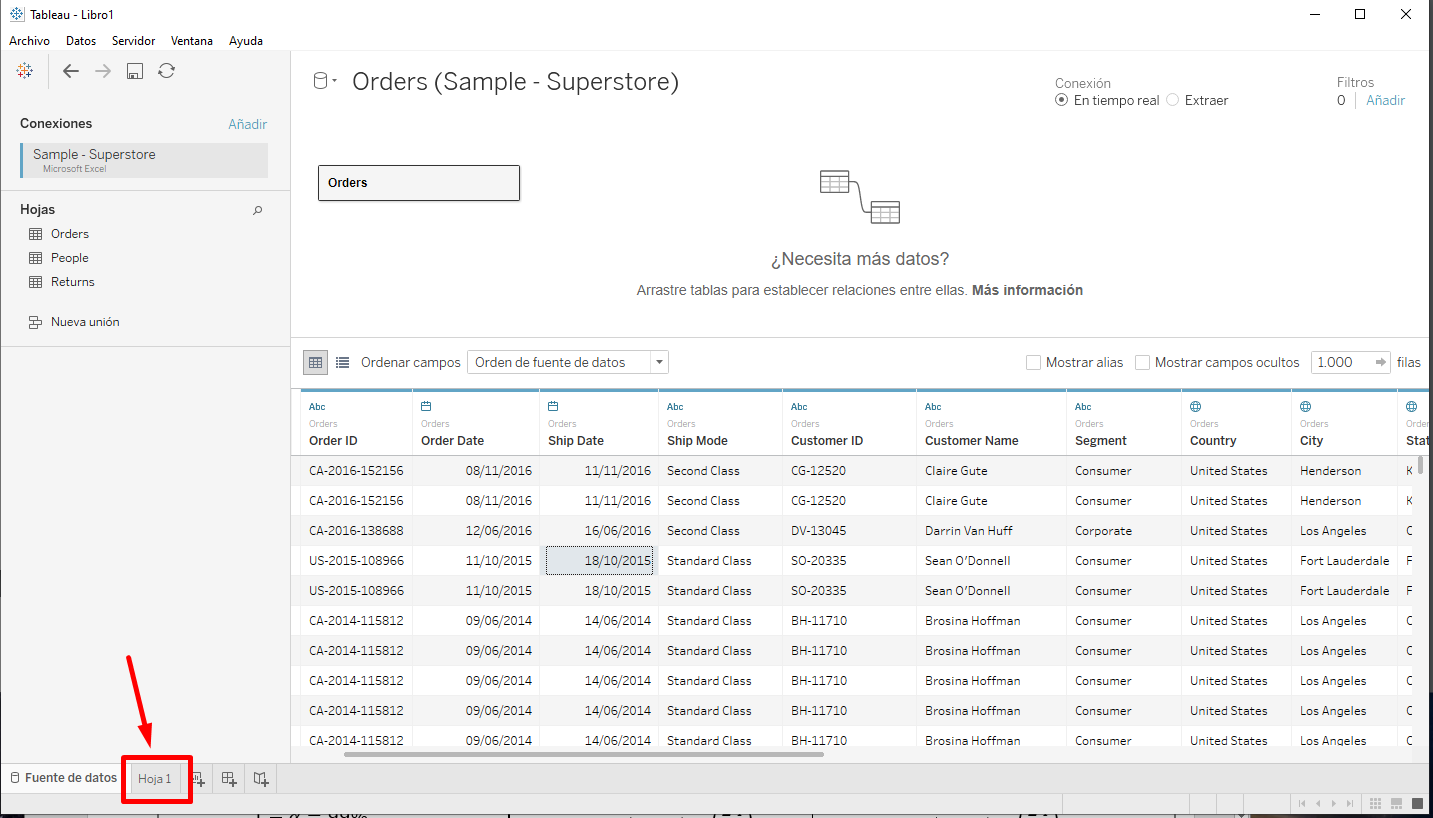
\includegraphics[width=15cm]{./img/img8.png}
        \end{center}
        \item Una vez que esté en la hoja de trabajo, desde \textit{\textbf{Dimensions}} debajo del panel Datos, arrastre \textit{\textbf{Order Date}} al estante Columna.
        \begin{center}
            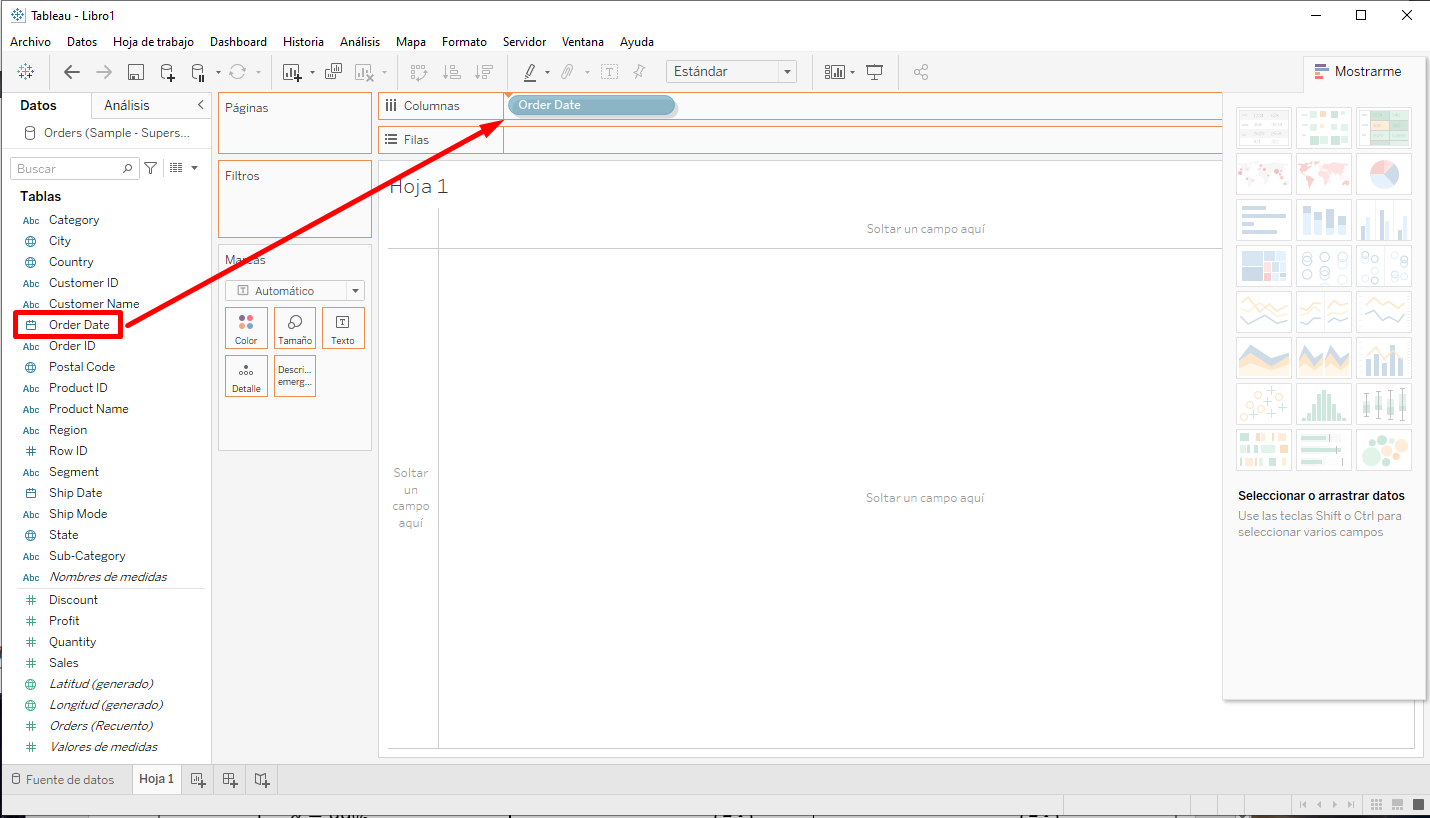
\includegraphics[width=15cm]{./img/img9.png}
        \end{center}
        \item Del mismo modo, desde la pestaña \textit{\textbf{Measures}}, arrastre el campo \textit{\textbf{Sales}} al estante Filas.
        \begin{center}
            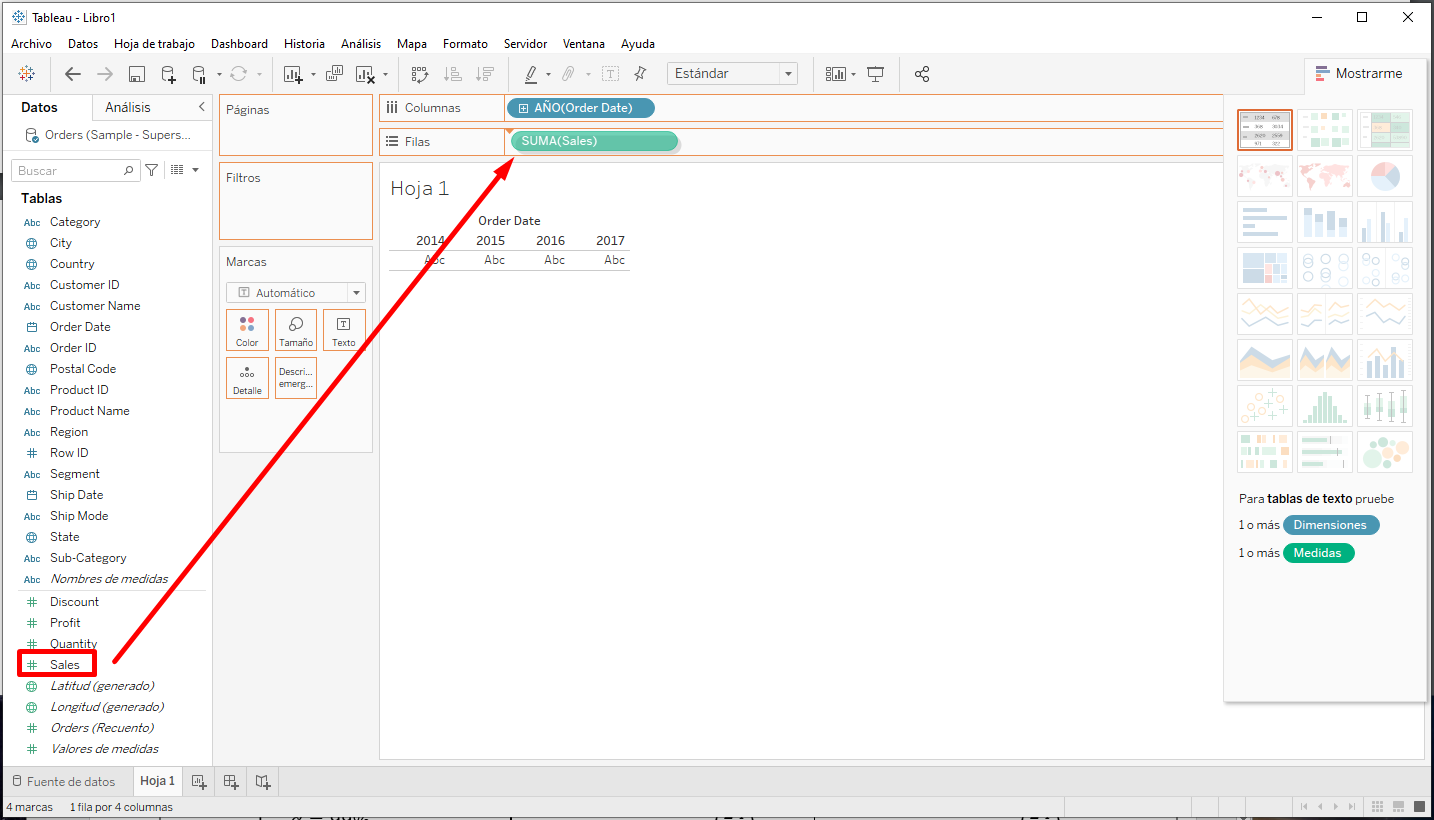
\includegraphics[width=15cm]{./img/img10.png}
        \end{center}
        \item Tableau completa un gráfico con las ventas agregadas como una suma. Se muestran las ventas totales agregadas de cada año por fecha de pedido. Tableau siempre completa un gráfico de líneas para una vista que incluye un campo de tiempo, que en este ejemplo es la fecha del pedido.
        \begin{center}
            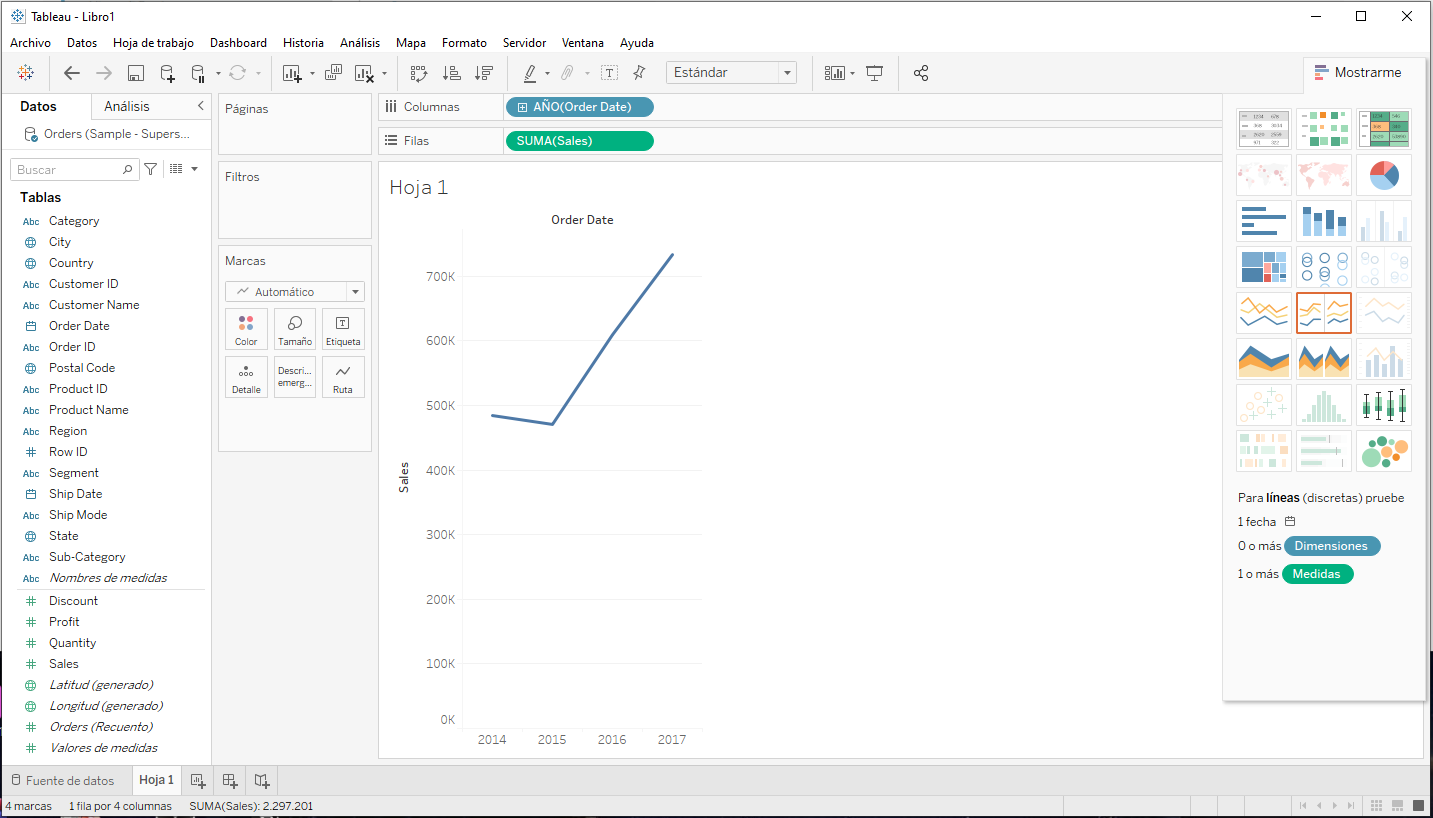
\includegraphics[width=15cm]{./img/img11.png}
        \end{center}
    \end{enumerate}
    %--------------------------------------------------------------------------------------------------------------------------------------------------------------------------------------------------------------------------------------------------------------------------------------------------------------------------------------------------------------------------------------------------------------------------------------------------------------------------------------------------------------
    \paragraph{\Large Refinando la vista\\ \\}
    Profundicemos e intentemos obtener más información sobre qué productos generan más ventas. Comencemos agregando las categorías de productos para ver los totales de ventas de una manera diferente.
    \begin{enumerate}
        \item \textit{\textbf{Category}} está presente en el panel \textbf{Dimensiones}. Arrástrelo al estante de columnas y colóquelo junto a \textit{\textbf{YEAR(Order Date)}}. El campo \textit{\textbf{Category}} debe ser colocado a la derecha de \textit{\textbf{Year}}.
        \begin{center}
            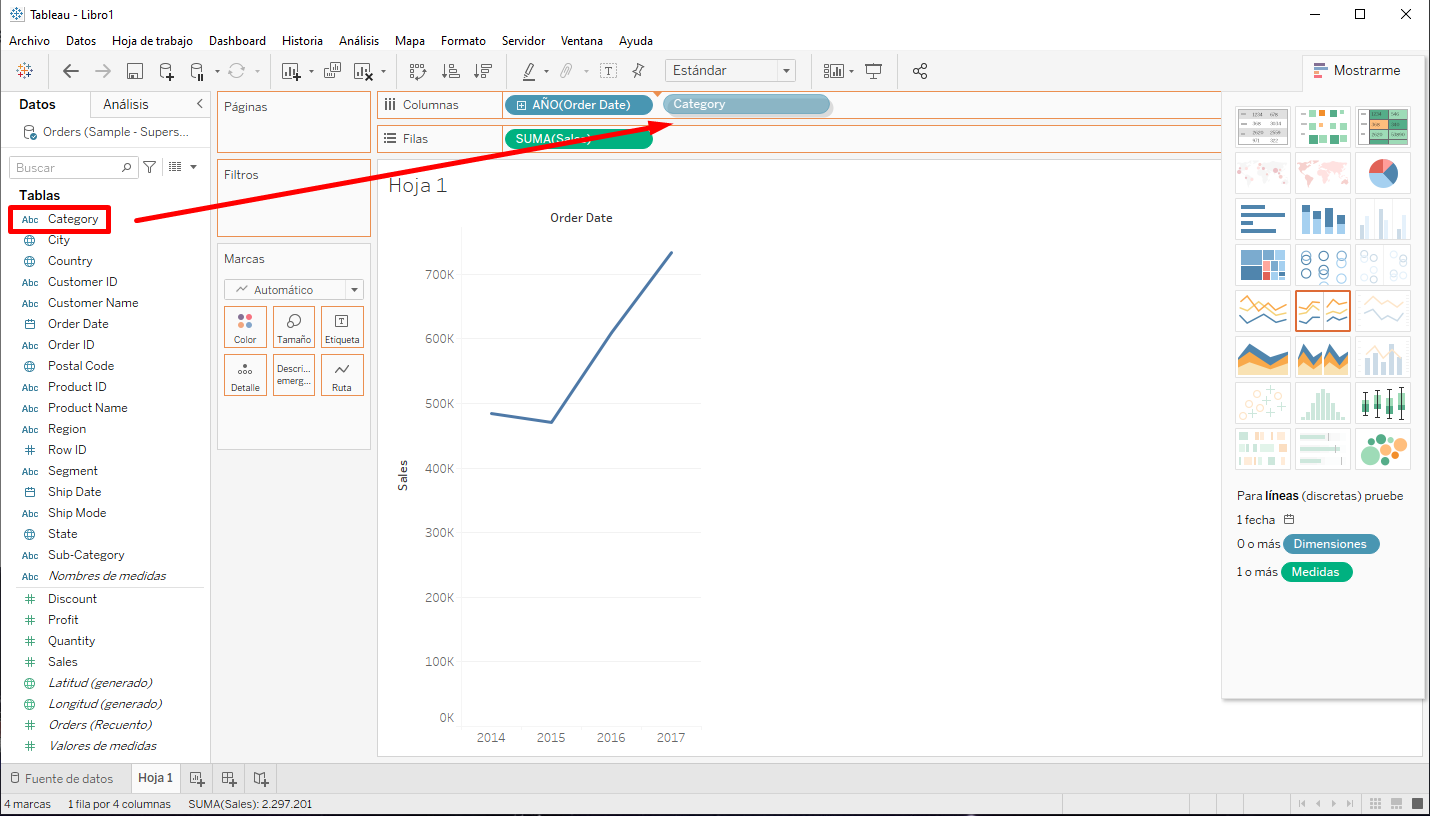
\includegraphics[width=15cm]{./img/img12.png}
        \end{center}
        \item Al hacerlo, la vista cambia inmediatamente a un tipo de gráfico de barras desde una línea. El gráfico muestra el total \textit{\textbf{Sales}} de cada \textit{\textbf{Product}} año.
        \begin{center}
            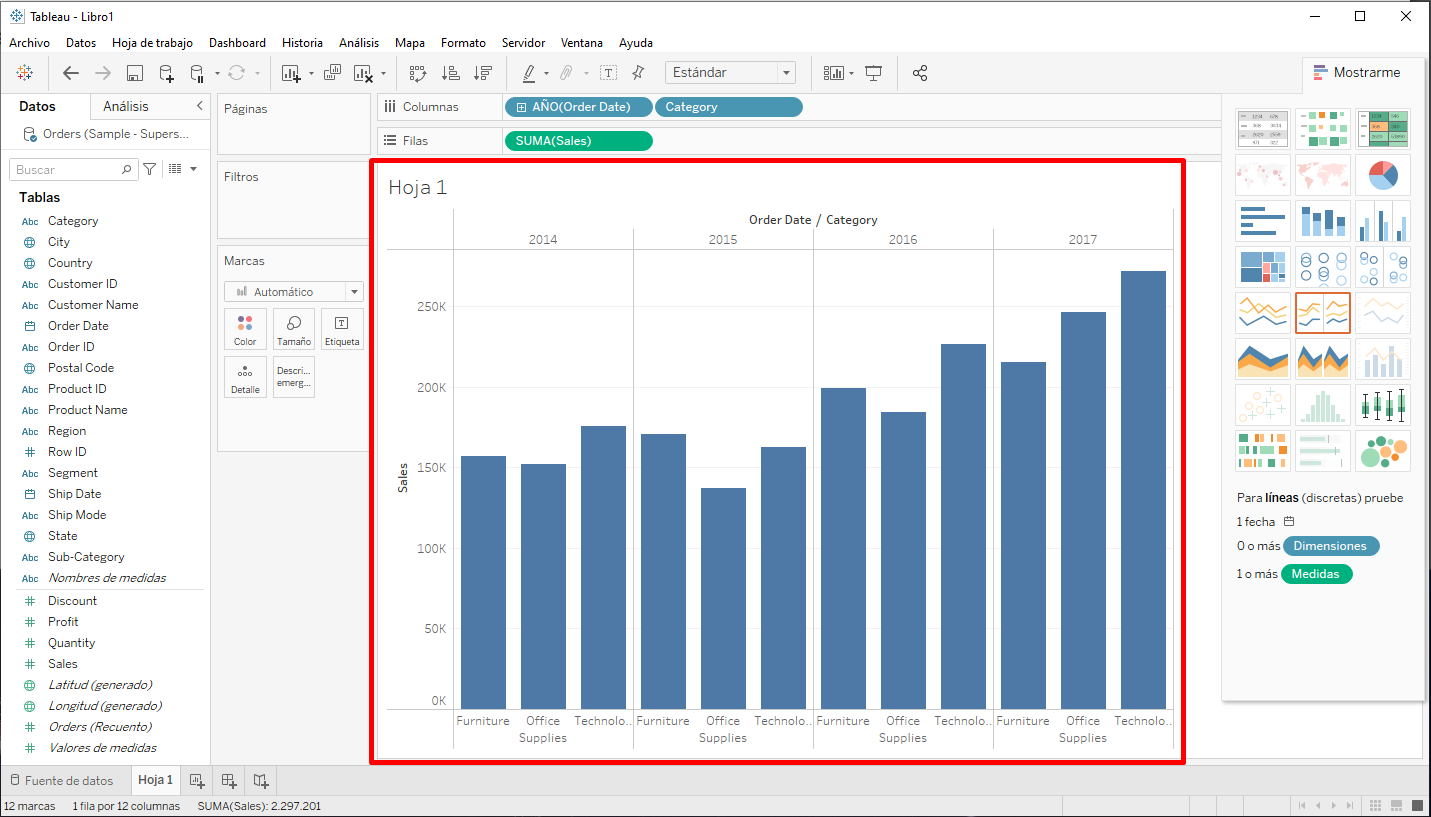
\includegraphics[width=15cm]{./img/img13.png}
        \end{center}
        \begin{itemize}
            \item Para ver información sobre cada punto de datos (es decir, una marca) en la vista, coloque el cursor sobre una de las barras para revelar una información sobre herramientas. La información sobre herramientas muestra las ventas totales para esa categoría. Aquí está la información sobre herramientas para la categoría Suministros de oficina para 2016:
            \begin{center}
                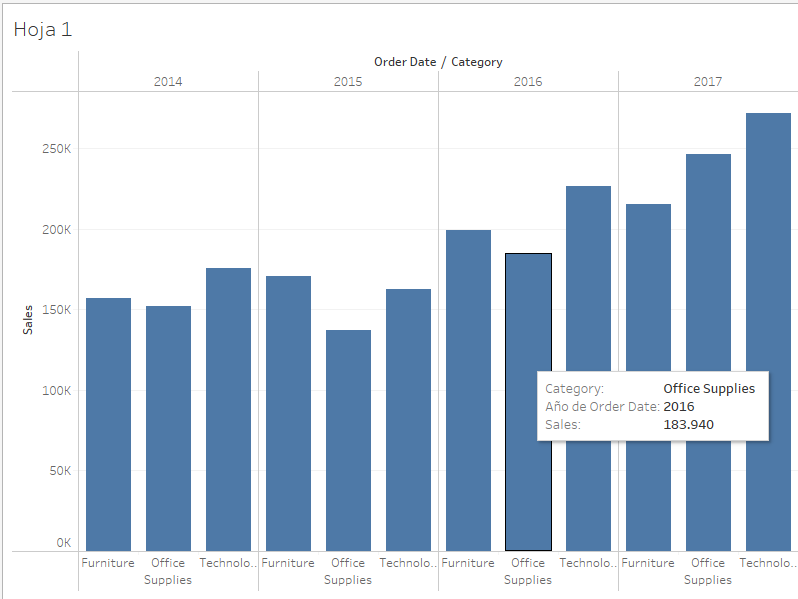
\includegraphics[width=15cm]{./img/img14.png}
            \end{center}
            \item Para agregar etiquetas a la vista, haga clic \textit{\textbf{Show Mark Labels}} en en la barra de herramientas.
            \begin{center}
                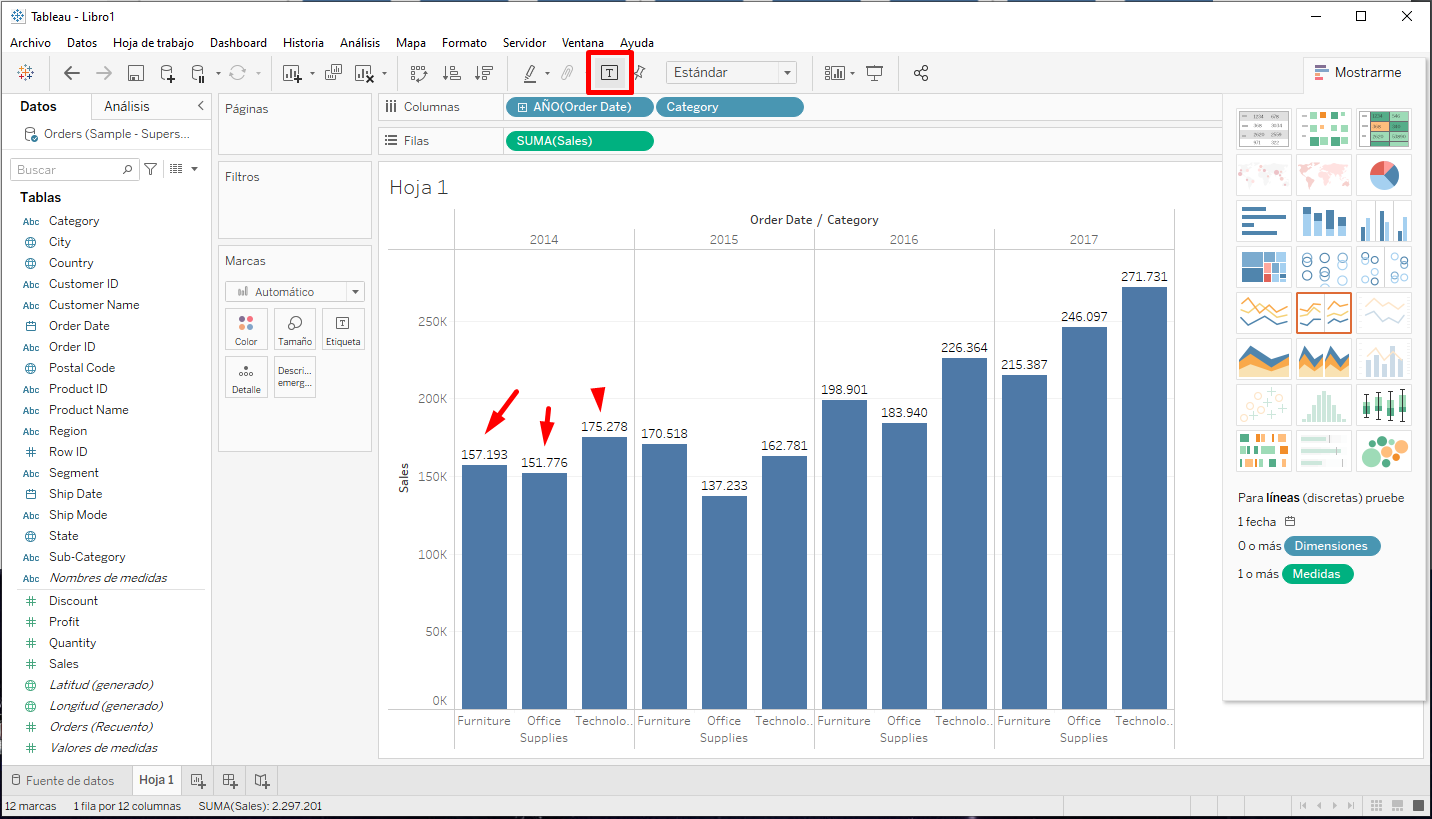
\includegraphics[width=15cm]{./img/img15.png}
            \end{center}
            \item El gráfico de barras también se puede mostrar horizontalmente en lugar de verticalmente. Haga clic \textit{\textbf{Swapen}} la barra de herramientas para el mismo.
            \begin{center}
                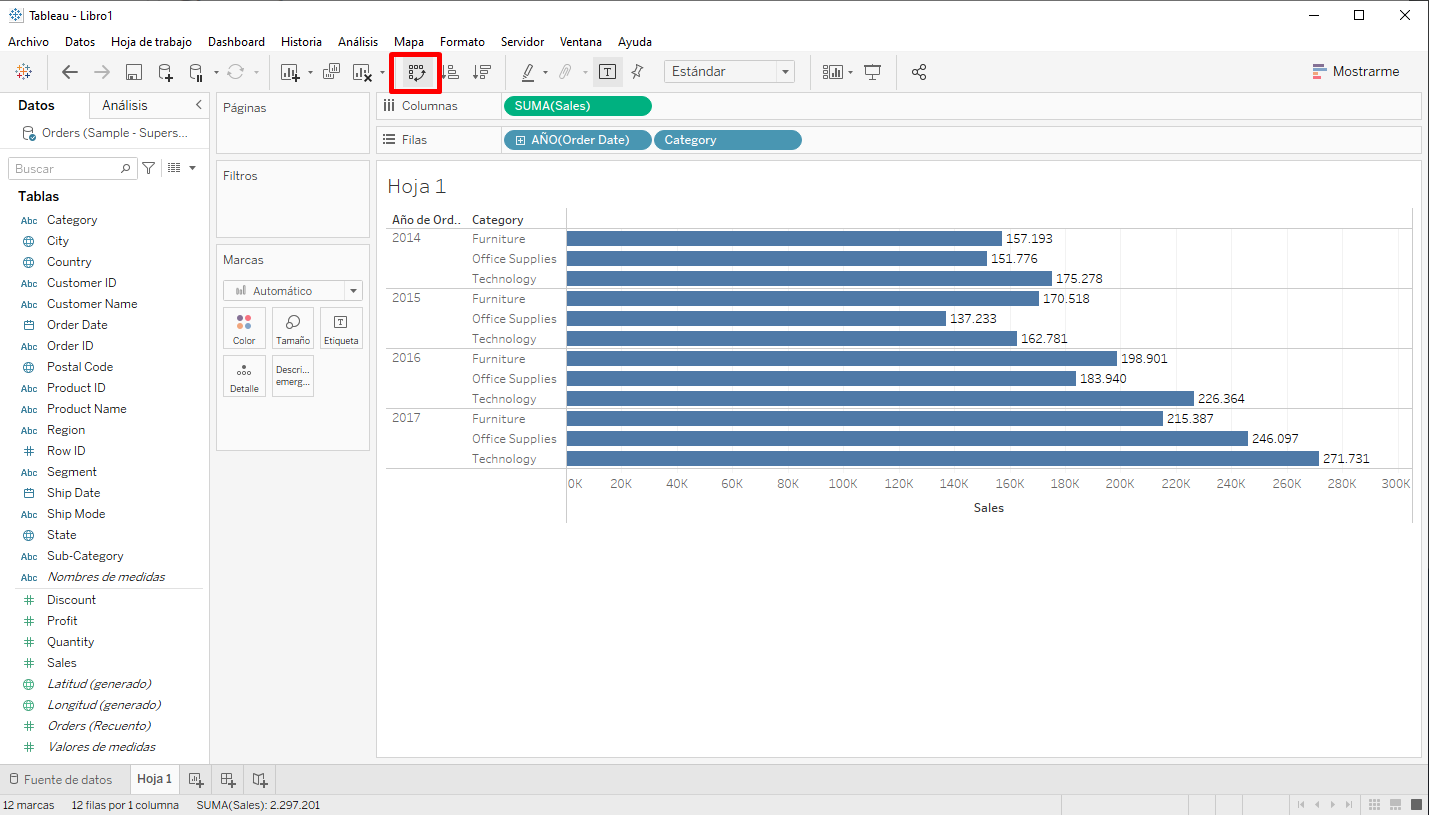
\includegraphics[width=15cm]{./img/img16.png}
            \end{center}
        \end{itemize}
        \item La vista por encima de Niza los espectáculos \textit{\textbf{sales}} de \textit{\textbf{category}}, por ejemplo, muebles, equipos de oficina, y la tecnología. También podemos inferir que las ventas de muebles están creciendo más rápido que las ventas de suministros de oficina, excepto en 2016. Por lo tanto, sería prudente centrar los esfuerzos de ventas en muebles en lugar de suministros de oficina. Pero los muebles son una categoría amplia y se componen de muchos elementos diferentes. ¿Cómo podemos identificar qué mueble está contribuyendo a las ventas máximas?.
        \begin{center}
            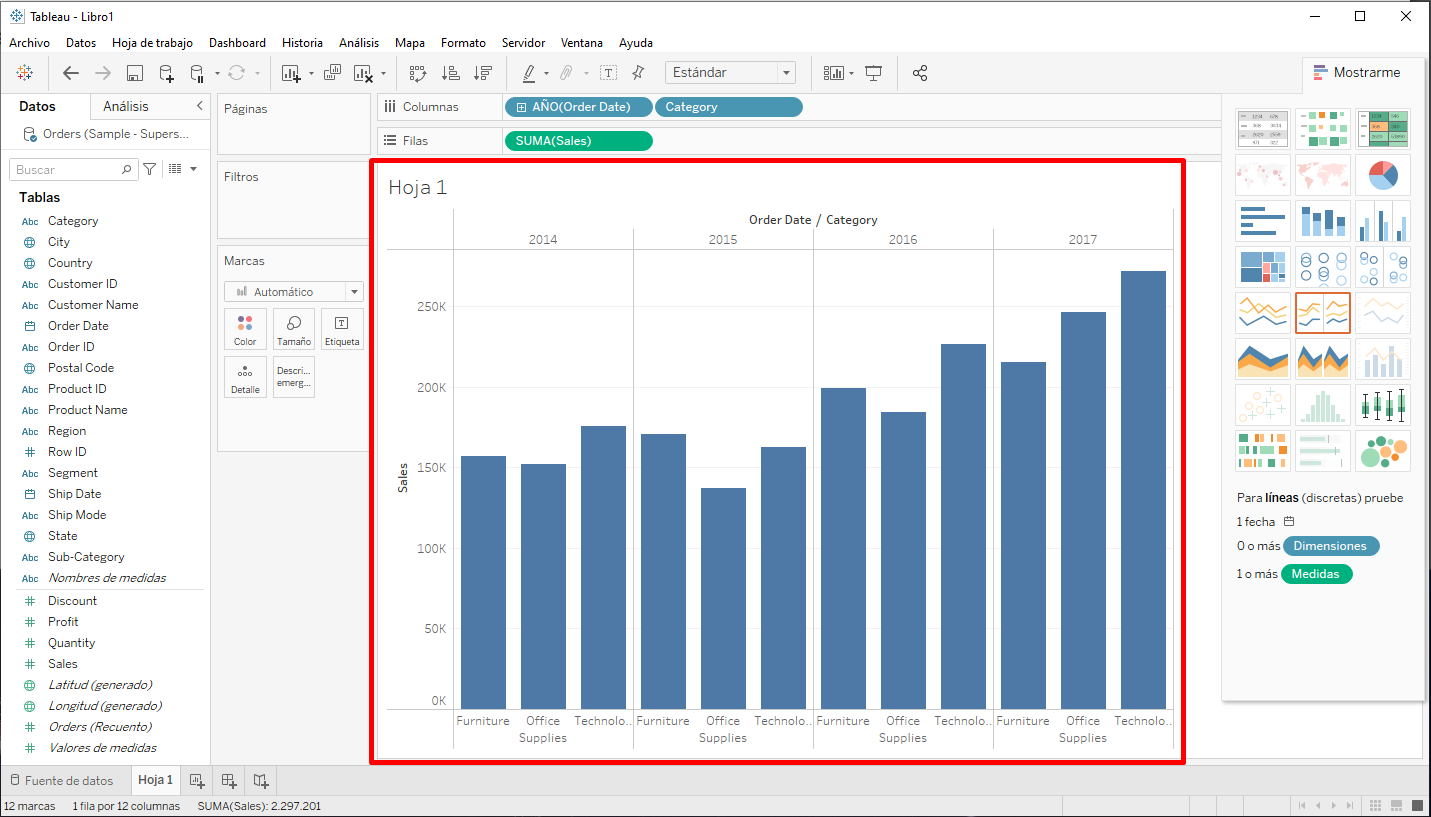
\includegraphics[width=15cm]{./img/img13.png}
        \end{center}
        \begin{itemize}
            \item Para ayudarnos a responder esa pregunta, decidimos mirar los productos \textit{\textbf{Sub-category}} para ver cuáles son los más vendidos. Digamos para la categoría \textbf{Mobiliario}; queremos ver los detalles únicamente sobre estanterías, sillas, muebles y mesas. Haremos doble clic o arrastraremos la \textit{\textbf{Sub-Category}} dimensión al estante Columnas.
            \begin{center}
                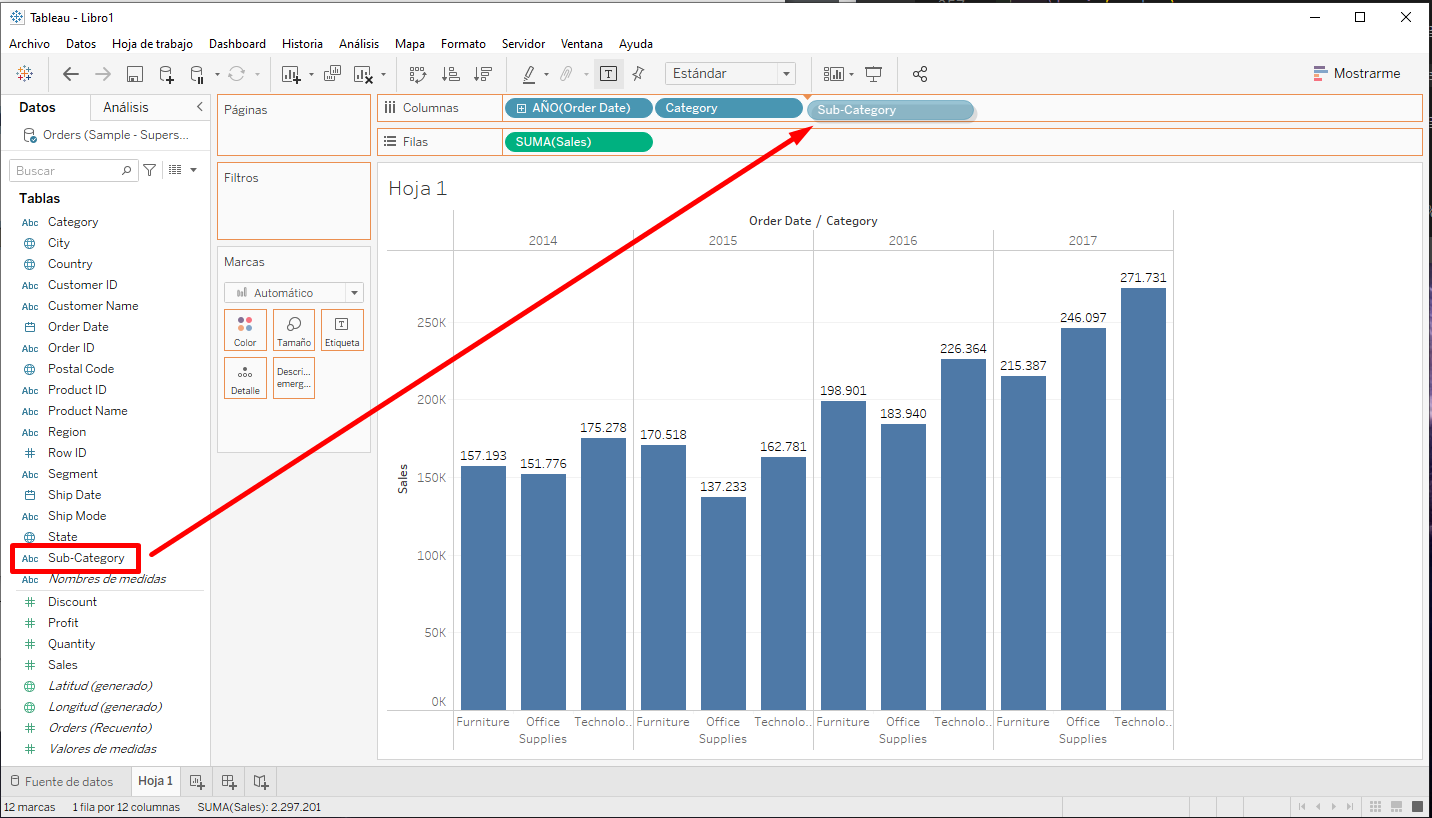
\includegraphics[width=15cm]{./img/img17.png}
            \end{center}
            \item La subcategoría es otro campo discreto. Además, analiza \textit{\textbf{Category}} y muestra una barra para cada uno \textit{\textbf{sub-category}} desglosado por categoría y año. Sin embargo, es una enorme cantidad de datos para entender visualmente. En la siguiente sección, aprenderemos sobre filtros, colores y otras formas de hacer que la vista sea más comprensible.
            \begin{center}
                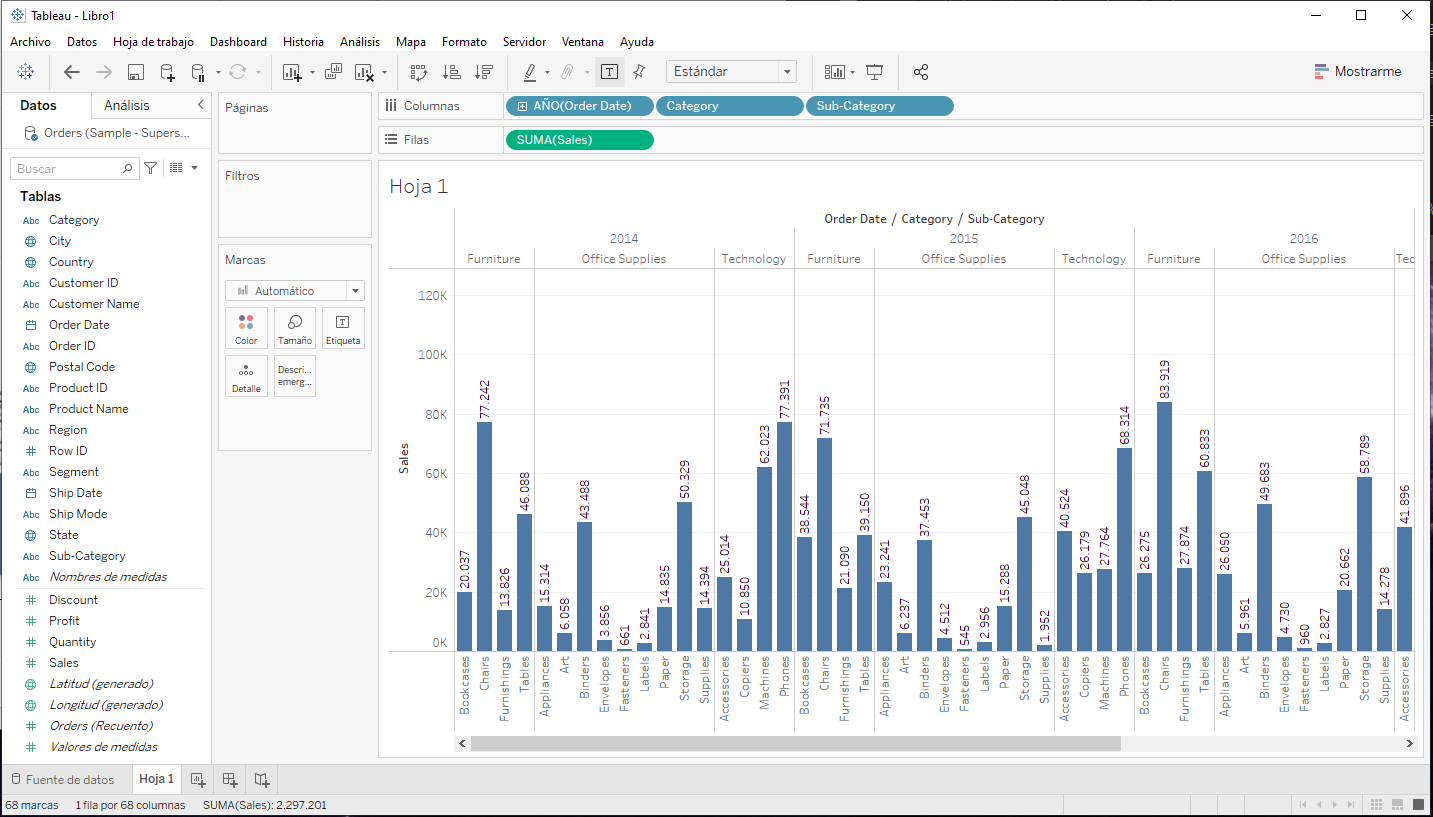
\includegraphics[width=15cm]{./img/img18.png}
            \end{center}
        \end{itemize}
    \end{enumerate}
    %%%%%%%%%%%%%%%%%%%%%%%%%%%%%%%%%%%%%%%%%%%%%%%%%%%%%%%%%%%%%%%%%%%%%%%%%%%%%%%%%%%%%%%%%%%%%%%%%%%%%%%%%%%%%%%%%%%%%%%%%%%%%%%%%%%%%%%%%%%%%%%%%%%%%%%%%%%%%%%%%%%%%%%%%%%%%%%%%%%%%%%%%%%%%%%%%%%%%%%%%%%%%%%%%%%%%%%%%%%%%%%%%%%%%%%%%%%%%%%%%%%%%%%%%%%%%%%%%%%%%%%%%%%%%%%%%%%%%%%%%%%%%%%%%%%%%%%%%%%%%%%%%%%%%%%%%%%%%%%%%%%%%%%%%%%%%%%%%%%%%%%%%%%%%%%%%%%%%%%%%%%%%%%%%%%%%%%%%%%%%%%%%%%%%%%%%%%%%%%%%%%%%%%%%%%%%%%%%%%%%%%%%%%%%%%%%%%%%%%%%%%%%%%%%%%%%%%%%%%%%%%%%%%%%%%%%%%%%%%%%%%%%%%%%%%%%%%
    \subsection{Enfatizando los resultados}
    En esta sección, intentaremos centrarnos en resultados específicos. Los filtros y colores son formas de agregar más enfoque a los detalles que nos interesan.
    \paragraph{\Large Agregar filtros a la vista\\ \\}
    Los filtros se pueden utilizar para incluir o excluir valores en la vista. Aquí intentamos agregar dos filtros simples a la hoja de trabajo para que sea más fácil ver las ventas de productos por subcategoría para un año específico.
    \begin{enumerate}
        \item En el panel Datos, en \textit{\textbf{Dimensiones}}, haga clic con el botón derecho en Order Date y seleccione Mostrar filtro. Repita también para el campo \textit{\textbf{Sub-Category}}.
        \begin{center}
            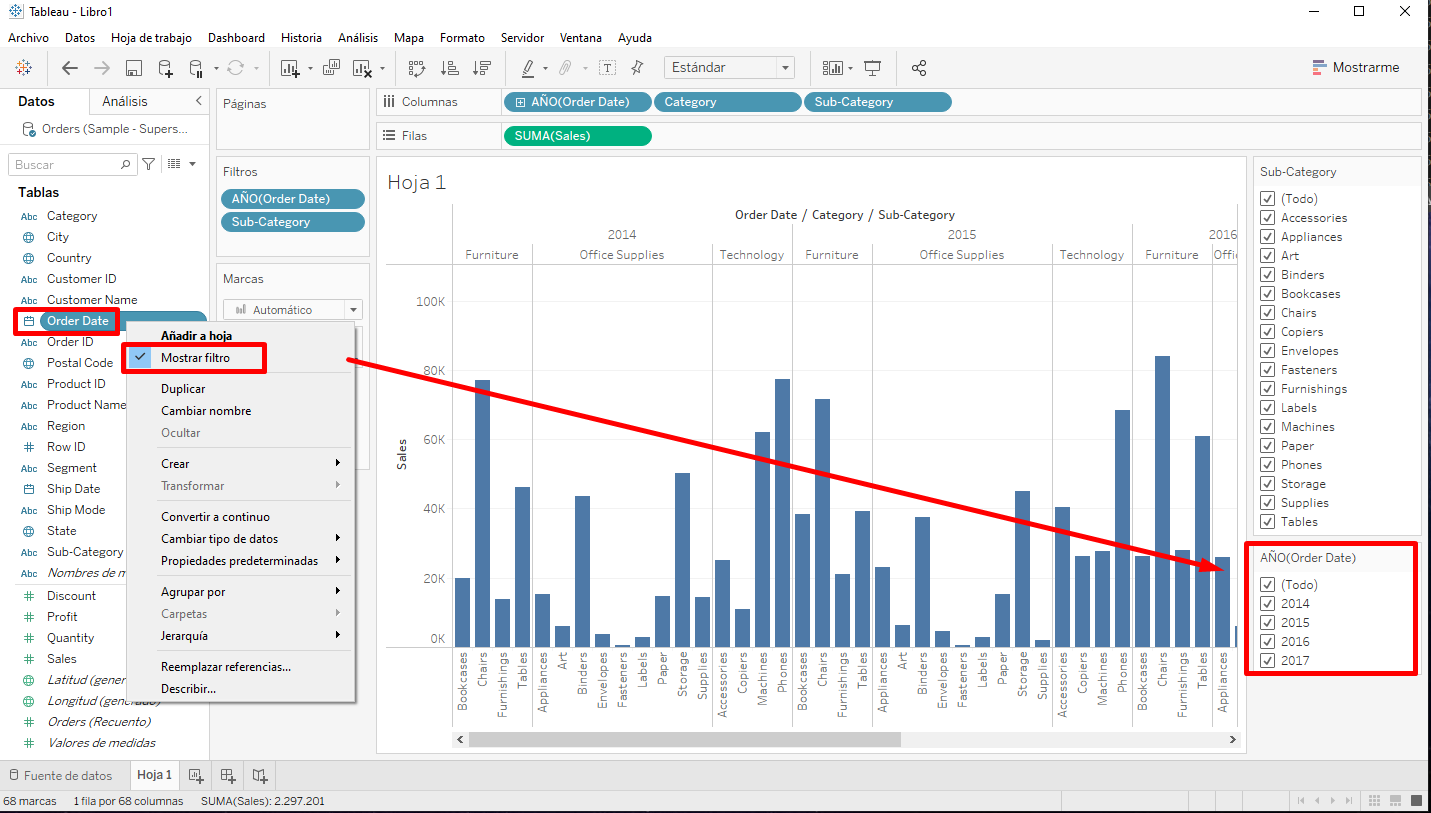
\includegraphics[width=15cm]{./img/img19.png}
        \end{center}
    \end{enumerate}
    %--------------------------------------------------------------------------------------------------------------------------------------------------------------------------------------------------------------------------------------------------------------------------------------------------------------------------------------------------------------------------------------------------------------------------------------------------------------------------------------------------------------
    \paragraph{\Large Agregar colores a la vista\\ \\}
    Los colores pueden ser útiles en la identificación visual de un patrón.
    \begin{enumerate}
        \item En el panel Datos, en Medidas, arrastre Beneficio a color en la tarjeta Marcas.
        \begin{center}
            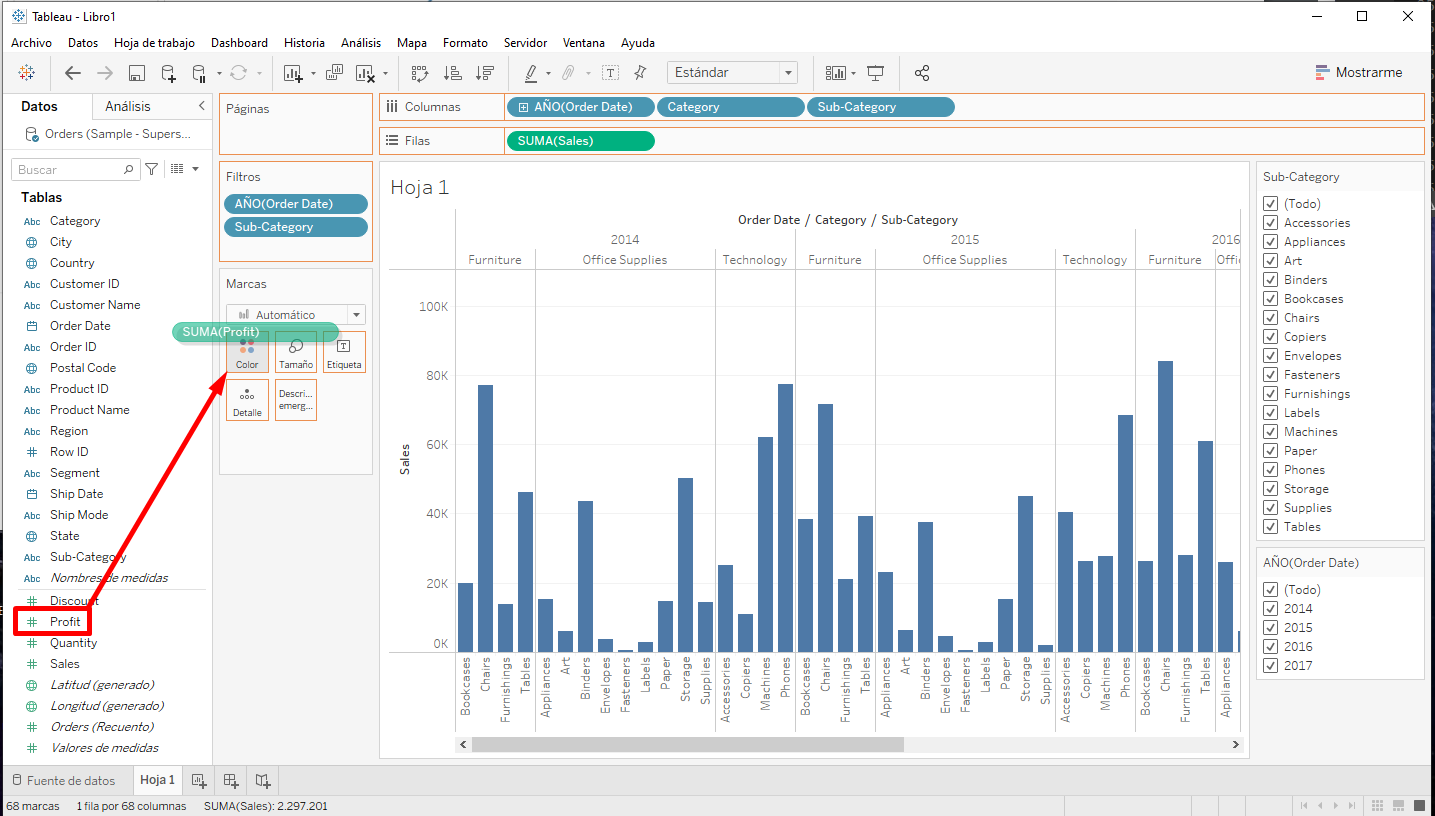
\includegraphics[width=15cm]{./img/img20.png}
        \end{center}
        \item Se puede ver que las estanterías, las mesas e incluso las máquinas contribuyen a la ganancia negativa, es decir, a la pérdida. Una visión poderosa.
        \begin{center}
            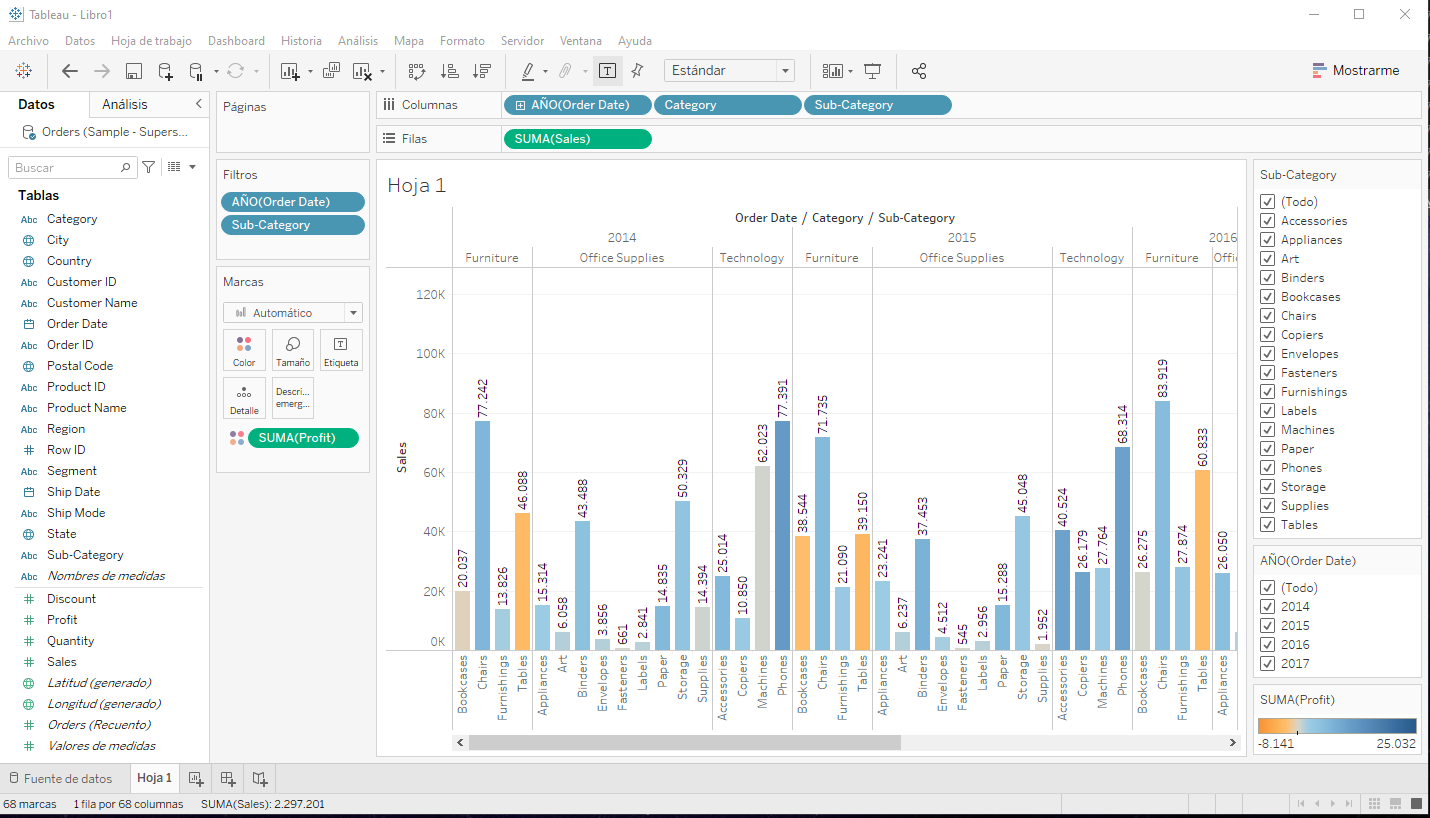
\includegraphics[width=15cm]{./img/img21.png}
        \end{center}
    \end{enumerate}
    %--------------------------------------------------------------------------------------------------------------------------------------------------------------------------------------------------------------------------------------------------------------------------------------------------------------------------------------------------------------------------------------------------------------------------------------------------------------------------------------------------------------
    \paragraph{\Large Resultados clave\\ \\}
    Echemos un vistazo más de cerca a los filtros para obtener más información sobre los productos no rentables.
    \begin{enumerate}[\tab 1.]
        \item En la vista, en la \textit{\textbf{Sub-Category}} tarjeta de filtro, desactive todas las casillas excepto \textit{\textbf{Bookcases}}, \textit{\textbf{Tables}}, y \textit{\textbf{Machines}}. Esto saca a la luz un hecho interesante. Mientras que en algunos años, las librerías y las máquinas fueron realmente rentables. Sin embargo, en 2016, Machines dejó de ser rentable.
        \begin{center}
            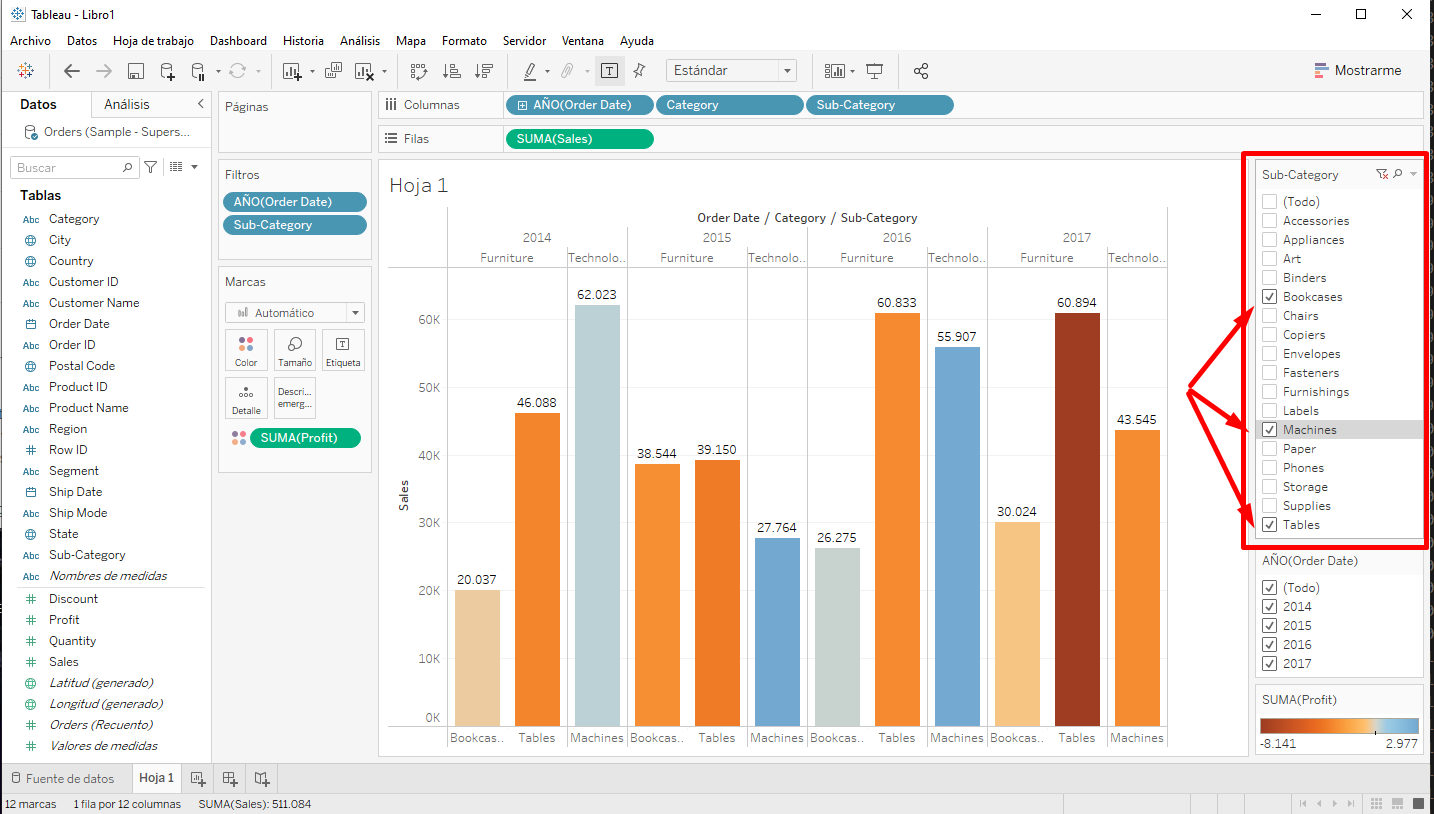
\includegraphics[width=15cm]{./img/img22.png}
        \end{center}
        \item Seleccione \textit{\textbf{All}} en la \textit{\textbf{Sub-Category}} tarjeta de filtro para mostrar todas las subcategorías nuevamente.
        \begin{center}
            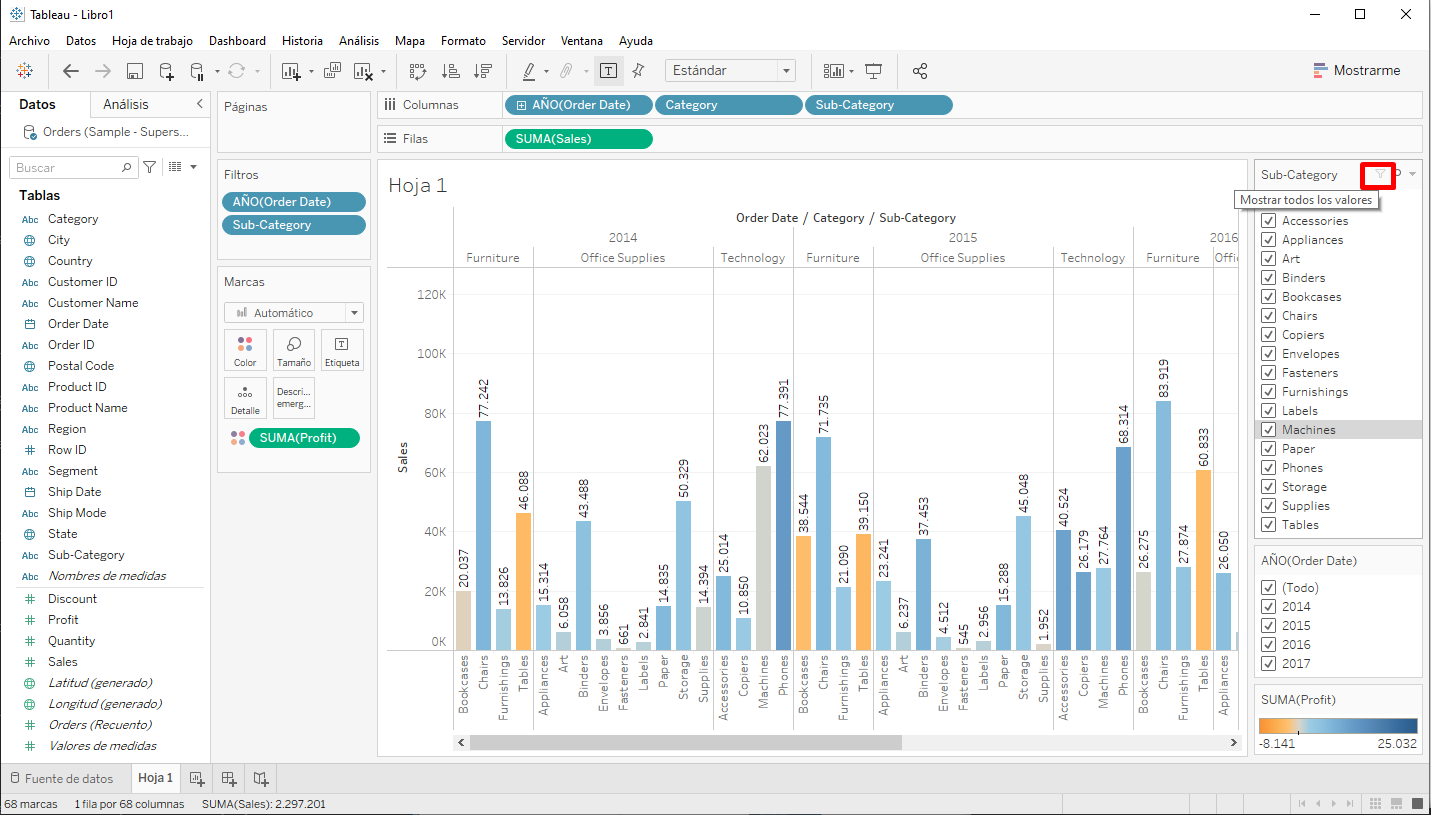
\includegraphics[width=15cm]{./img/img23.png}
        \end{center}
        \item Desde Dimensiones, arrastre {\textbf{Region}} al estante {\textbf{Rows}} y colóquelo a la izquierda de la pestaña Suma (Ventas). Observamos que las máquinas en el sur están reportando un beneficio negativo mayor en general que en sus otras regiones.
        \begin{center}
            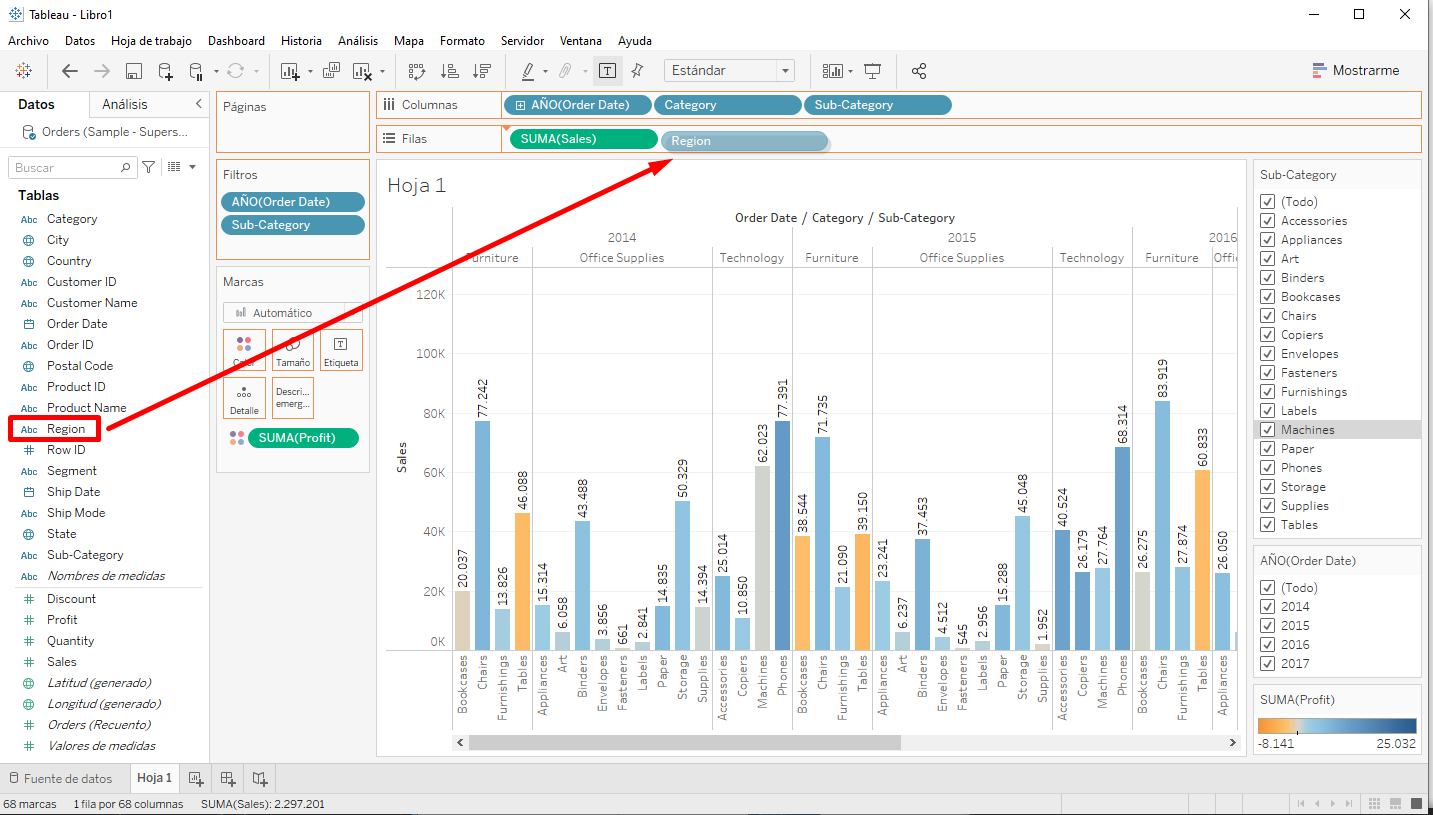
\includegraphics[width=15cm]{./img/img24.png}
        \end{center}
        \item Démosle ahora un nombre a la hoja. En la parte inferior izquierda del espacio de trabajo, haga doble clic {\textbf{Sheet 1}} y escriba {\textbf{Sales by Product and Region}}.
        \begin{center}
            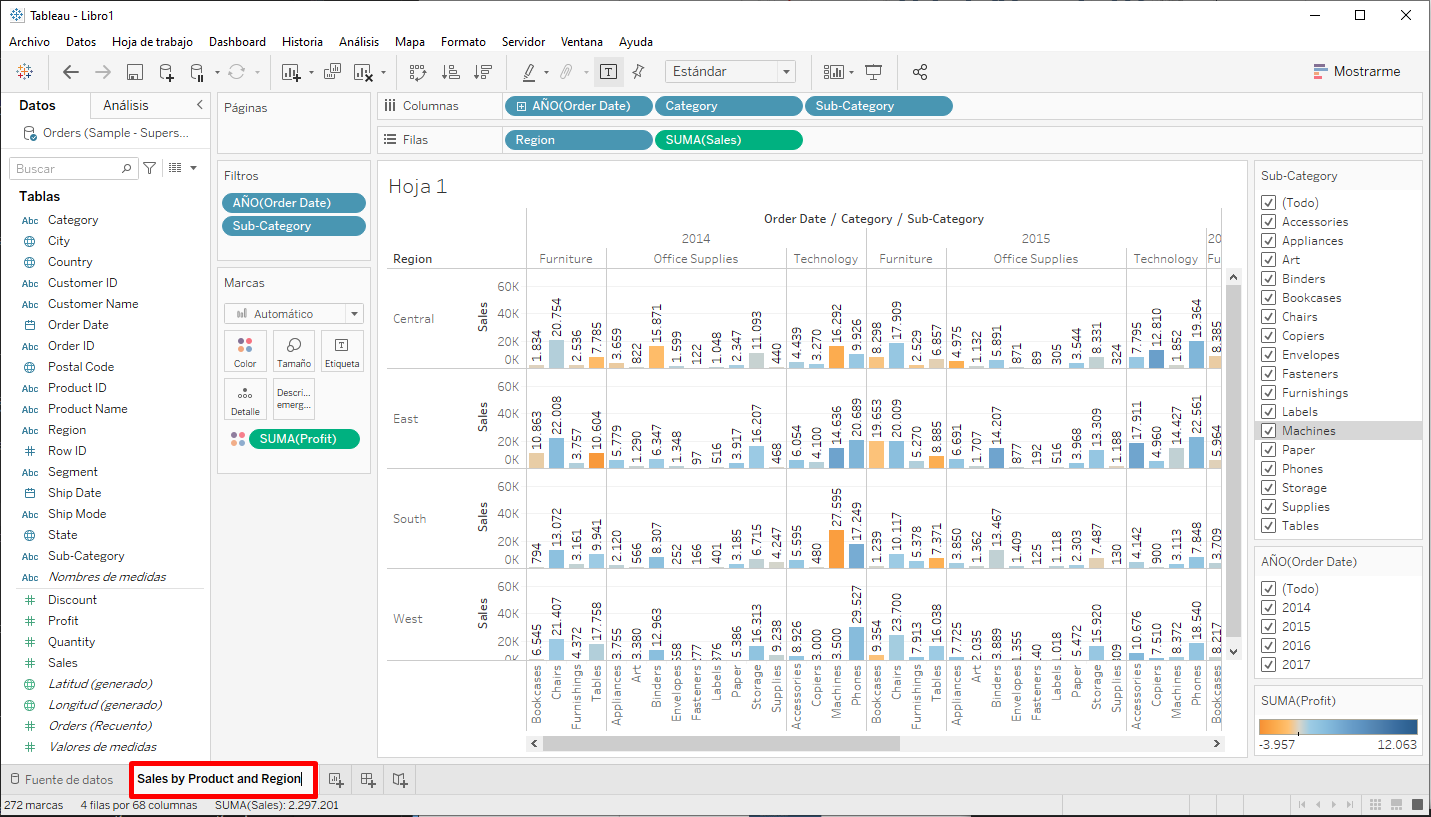
\includegraphics[width=15cm]{./img/img25.png}
        \end{center}
        \item Para conservar la vista, Tableau nos permite duplicar nuestra hoja de trabajo para que podamos continuar en otra hoja desde donde la dejamos. En su libro de trabajo, haga clic con el botón derecho en la hoja \textit{\textbf{Sales by Product and Region}} y seleccione \textit{\textbf{Duplicate}}.
        \begin{center}
            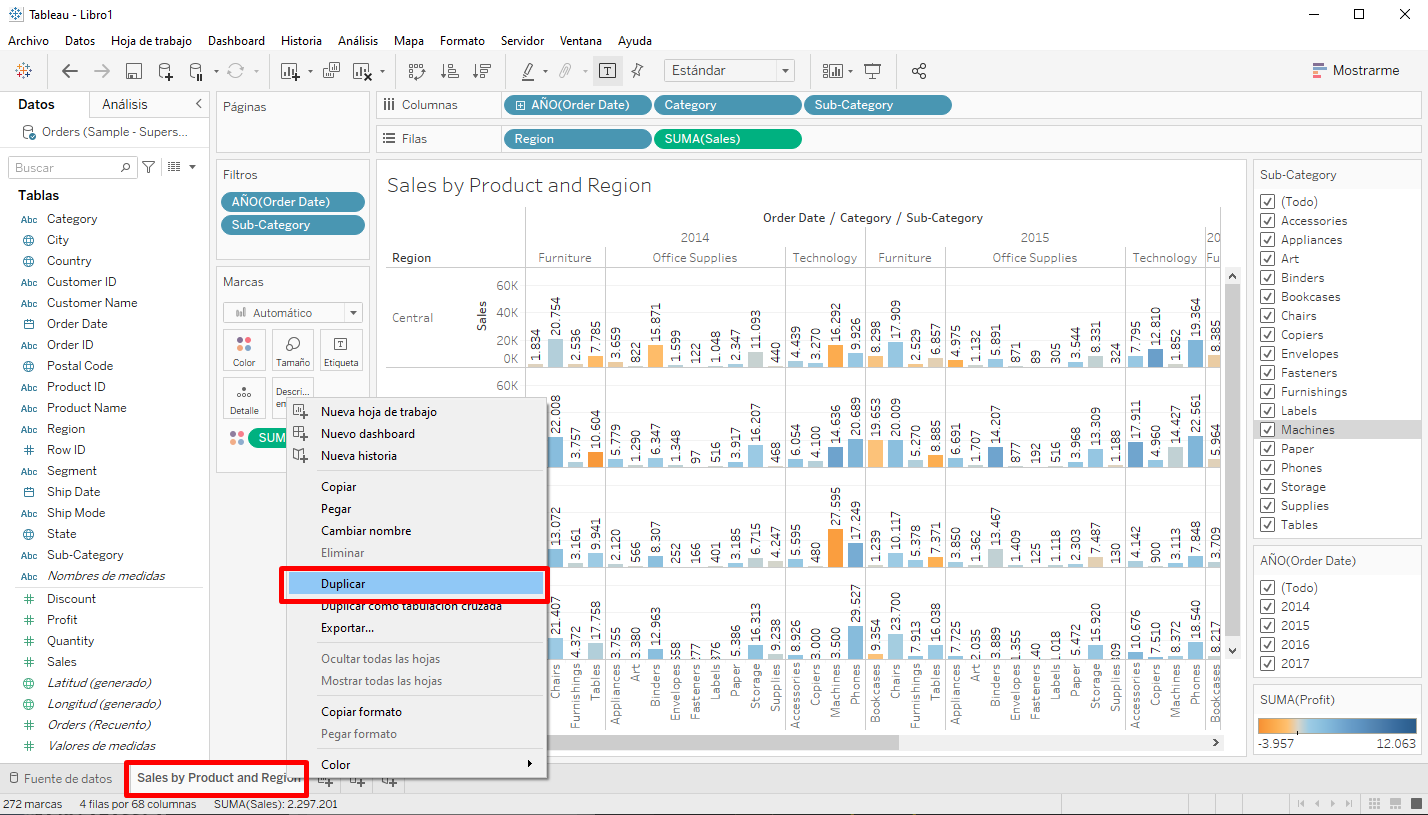
\includegraphics[width=15cm]{./img/img26.png}
        \end{center}
        \item Cambie el nombre de la hoja duplicada a \textit{\textbf{SalesSouth}}.
        \begin{center}
            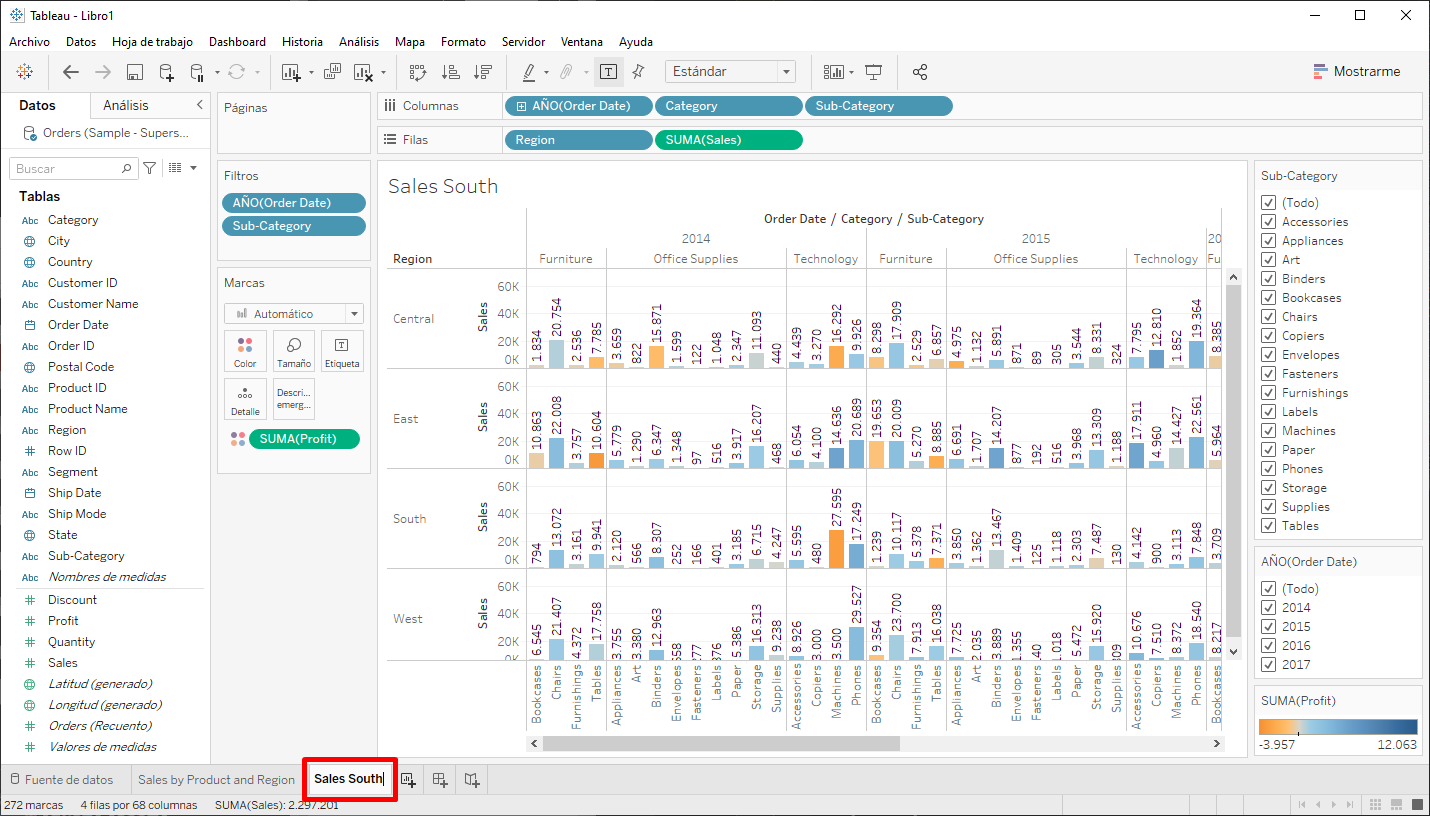
\includegraphics[width=15cm]{./img/img27.png}
        \end{center}
        \item En la nueva hoja de trabajo, desde Dimensiones, arrastre \textit{\textbf{Region}} al estante \textit{\textbf{Filters}} para agregarlo como un filtro en la vista.
        \begin{center}
            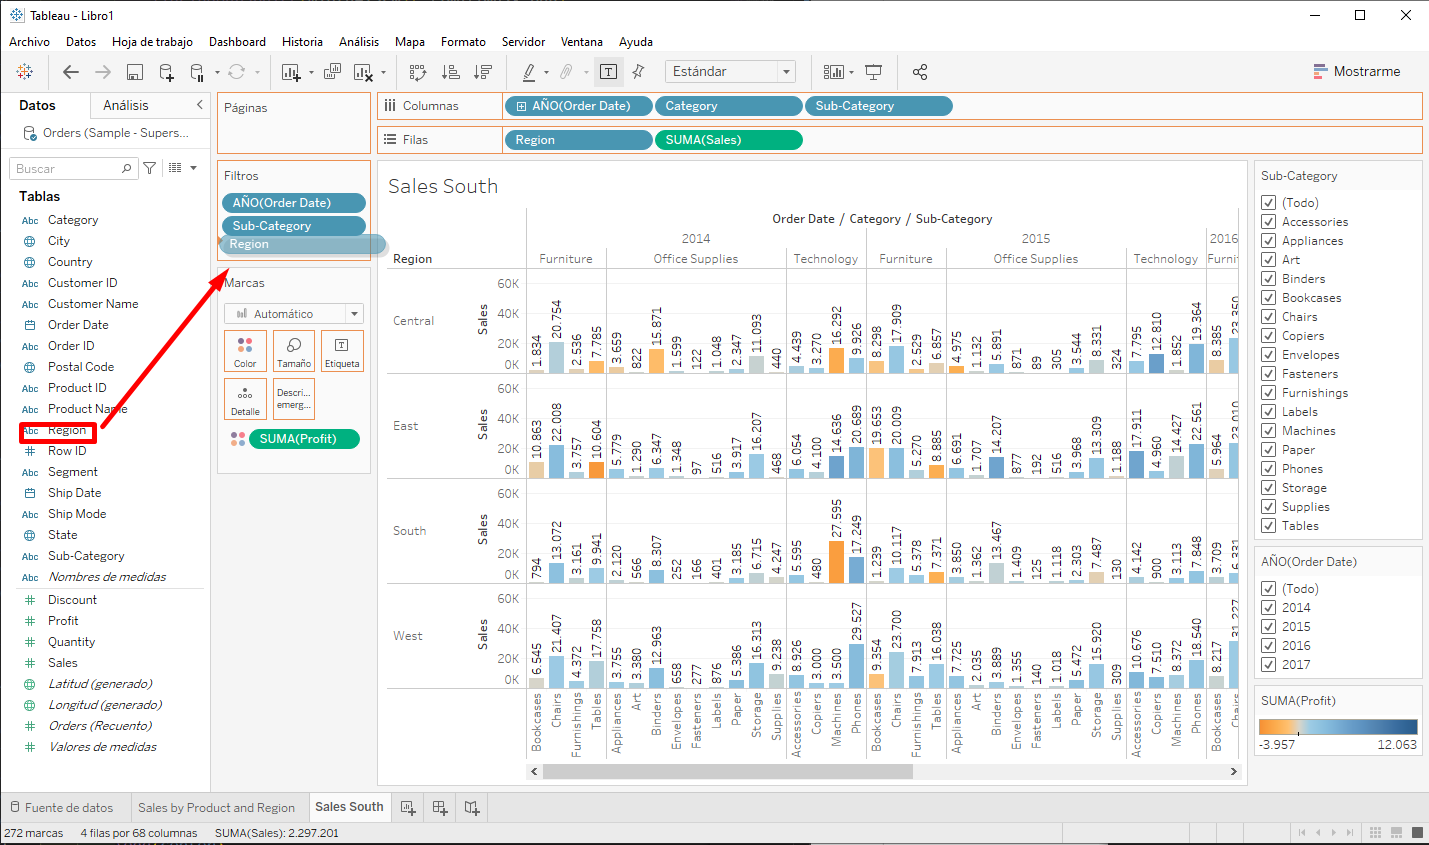
\includegraphics[width=15cm]{./img/img28.png}
        \end{center}
        \item En el cuadro de diálogo Región de filtro, desactive todas las casillas de verificación excepto Sur y luego haga clic en \textit{\textbf{OK}}. Ahora podemos centrarnos en las ventas y las ganancias en \textit{\textbf{South}}. Descubrimos que las ventas de máquinas tuvieron un beneficio negativo en 2014 y nuevamente en 2016.
        \begin{center}
            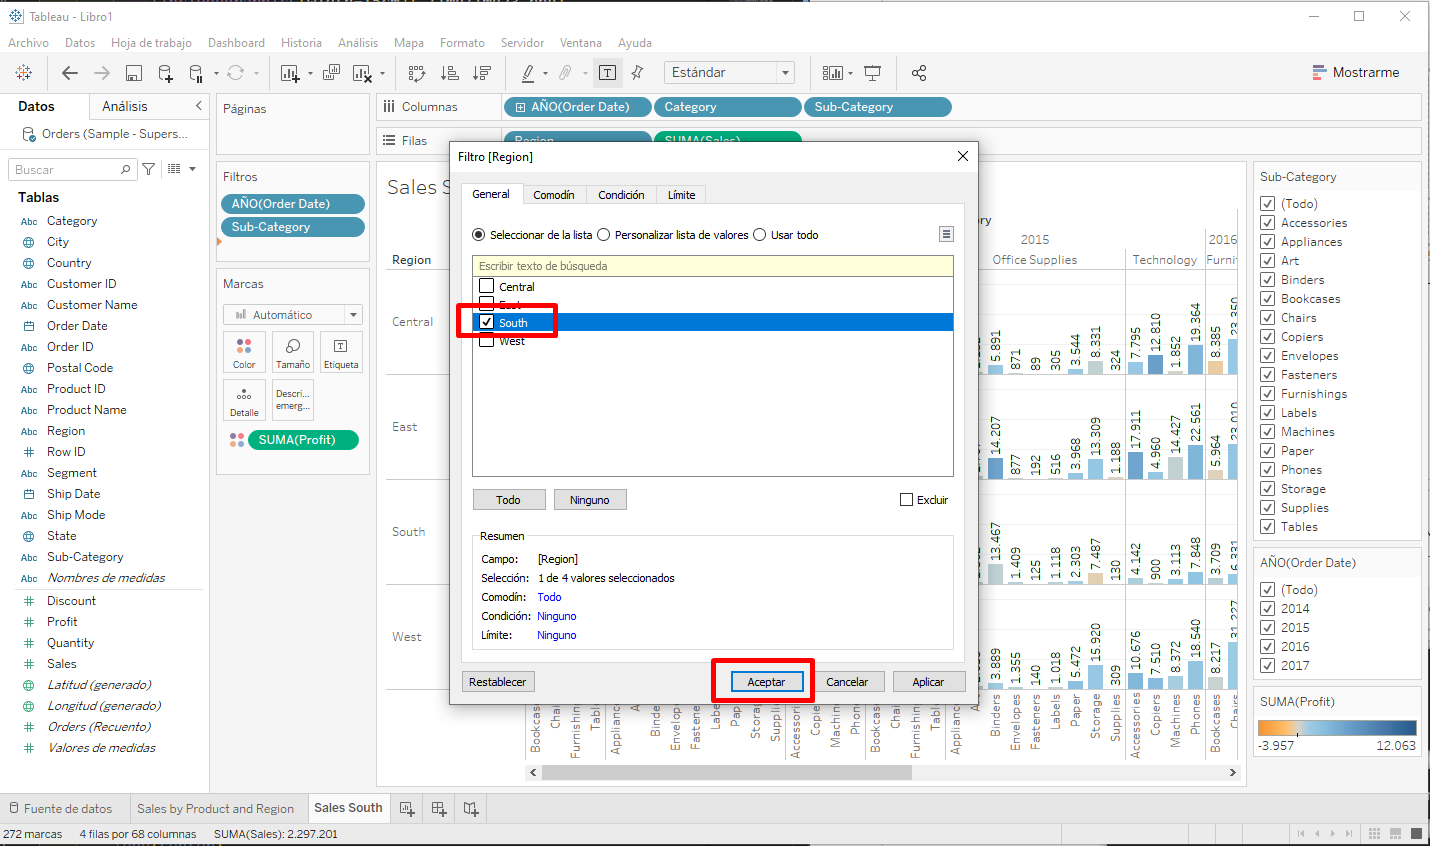
\includegraphics[width=15cm]{./img/img29.png}
        \end{center}
        \item Por último, no olvide guardar los resultados seleccionando \textit{\textbf{File > Save As}}.
        \begin{center}
            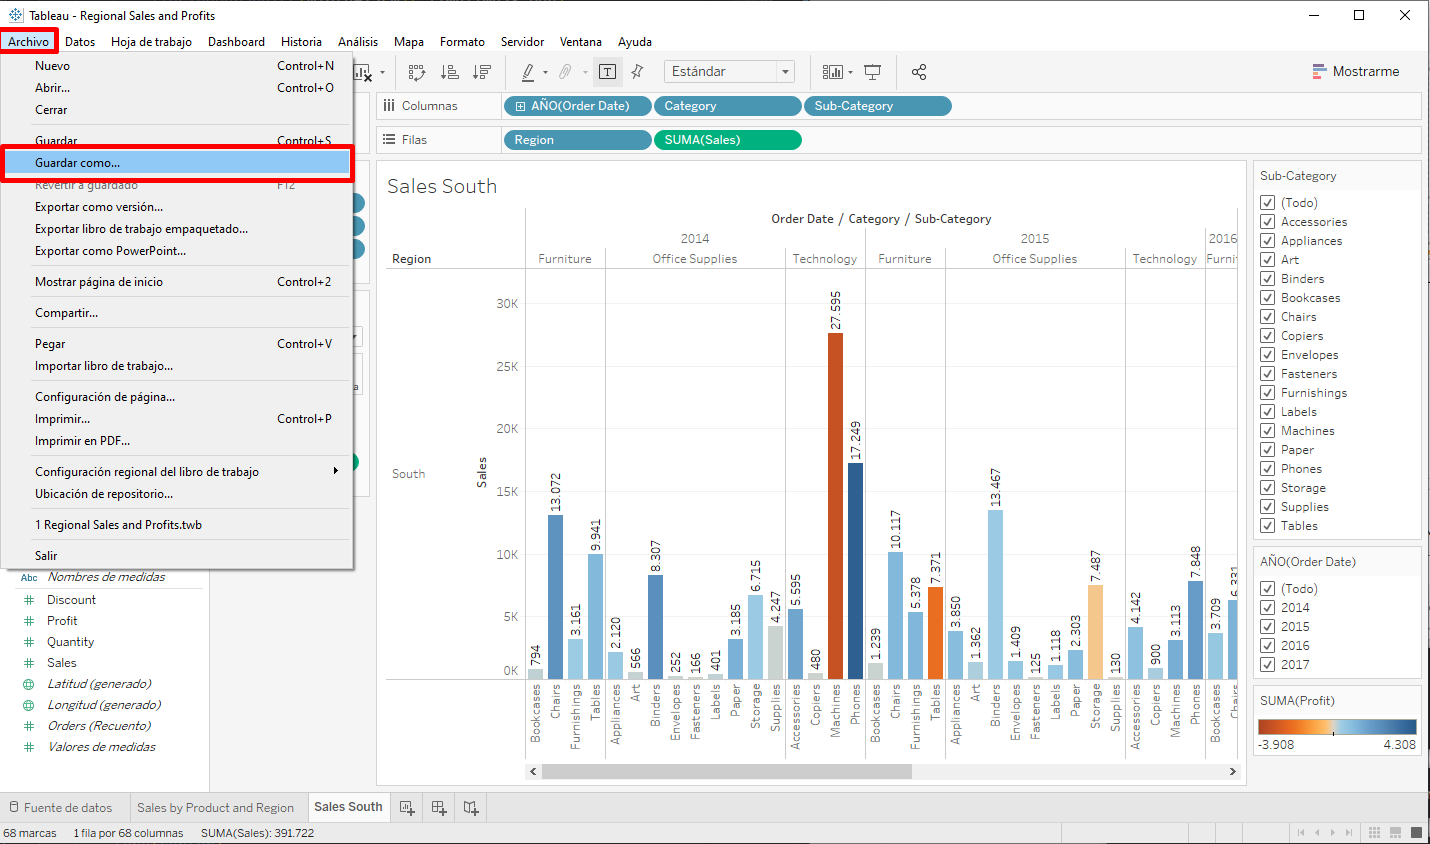
\includegraphics[width=15cm]{./img/img30.png}
        \end{center}
        \item Nombremos nuestro libro de trabajo como \textit{\textbf{Regional Sales and Profits}}.
        \begin{center}
            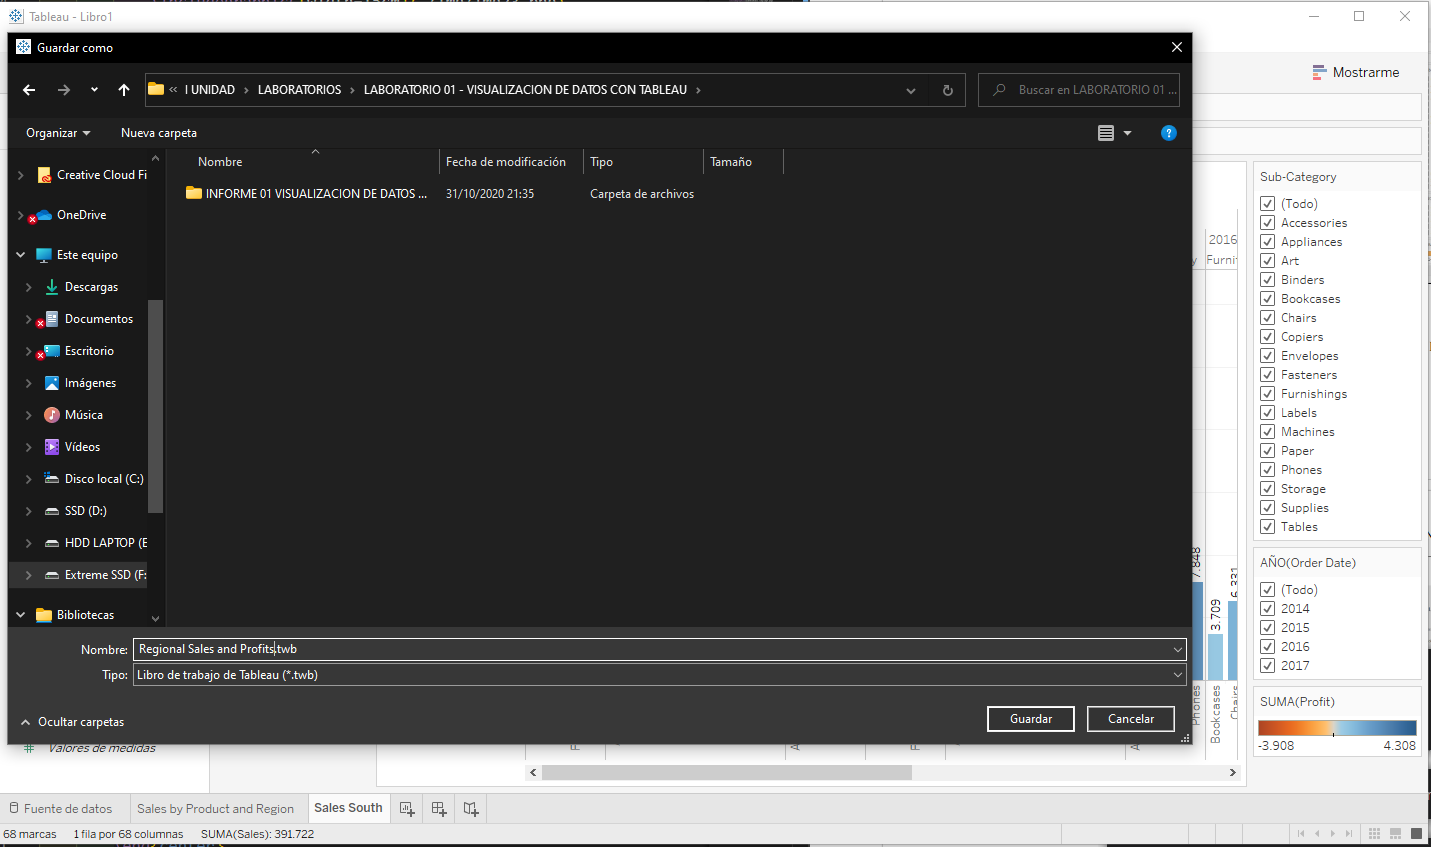
\includegraphics[width=15cm]{./img/img31.png}
        \end{center}
    \end{enumerate}
    %%%%%%%%%%%%%%%%%%%%%%%%%%%%%%%%%%%%%%%%%%%%%%%%%%%%%%%%%%%%%%%%%%%%%%%%%%%%%%%%%%%%%%%%%%%%%%%%%%%%%%%%%%%%%%%%%%%%%%%%%%%%%%%%%%%%%%%%%%%%%%%%%%%%%%%%%%%%%%%%%%%%%%%%%%%%%%%%%%%%%%%%%%%%%%%%%%%%%%%%%%%%%%%%%%%%%%%%%%%%%%%%%%%%%%%%%%%%%%%%%%%%%%%%%%%%%%%%%%%%%%%%%%%%%%%%%%%%%%%%%%%%%%%%%%%%%%%%%%%%%%%%%%%%%%%%%%%%%%%%%%%%%%%%%%%%%%%%%%%%%%%%%%%%%%%%%%%%%%%%%%%%%%%%%%%%%%%%%%%%%%%%%%%%%%%%%%%%%%%%%%%%%%%%%%%%%%%%%%%%%%%%%%%%%%%%%%%%%%%%%%%%%%%%%%%%%%%%%%%%%%%%%%%%%%%%%%%%%%%%%%%%%%%%%%%%%%%
    \subsection{Vista de mapa}
    \paragraph{\Large Crear una vista de mapa\\ \\}
    Las vistas de mapa son beneficiosas cuando buscamos datos geográficos (el campo Región). En el ejemplo actual, Tableau reconoce automáticamente que los campos País, Estado, Ciudad y Código postal contienen información geográfica.
    \begin{enumerate}
        \item Crea una nueva hoja de trabajo.
        \begin{center}
            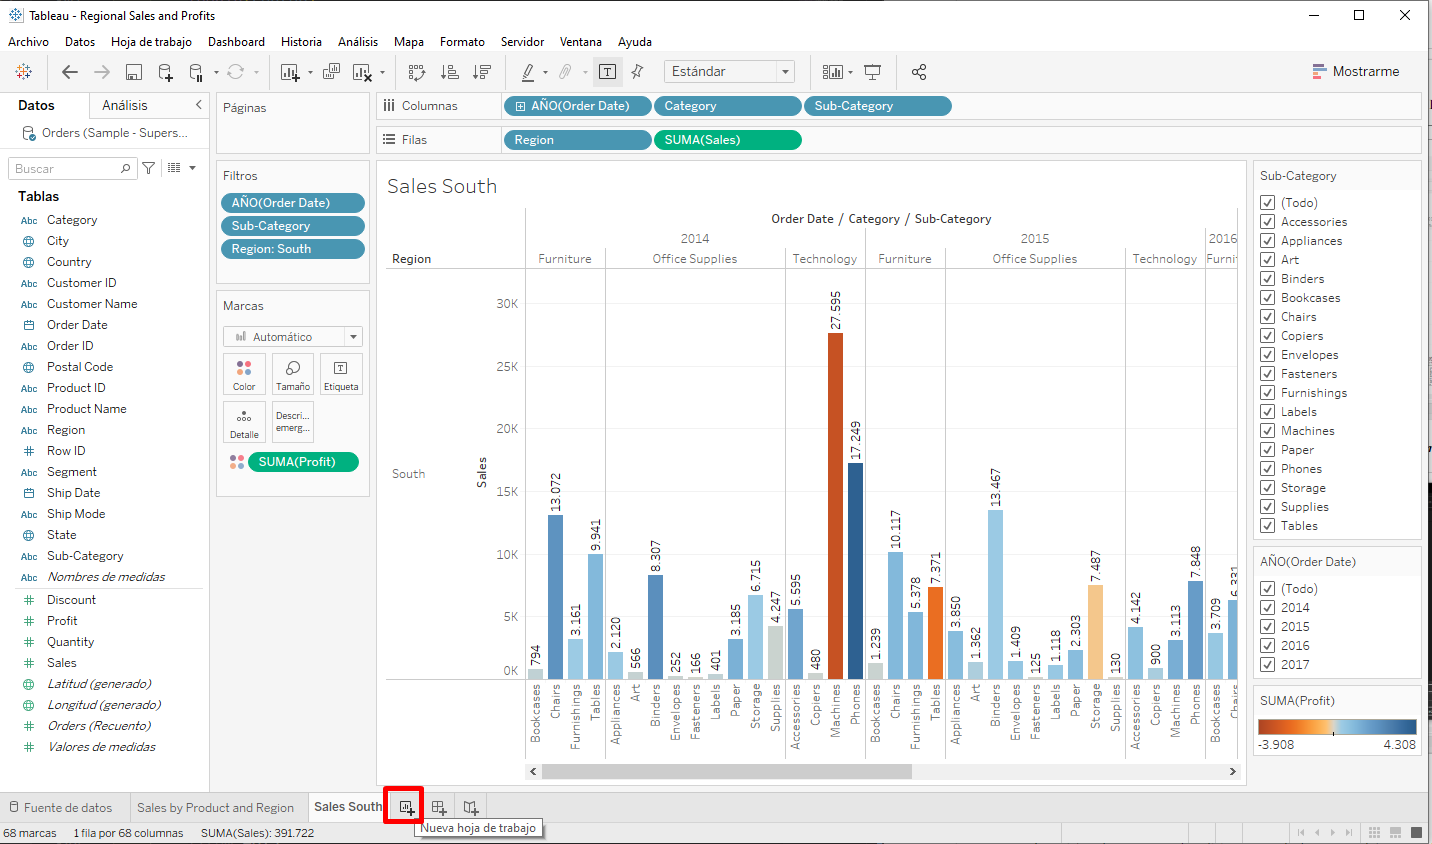
\includegraphics[width=15cm]{./img/img32.png}
        \end{center}
        \item Agregue \textit{\textbf{State}} y \textit{\textbf{Country}} en el panel Datos a \textit{\textbf{Detail}} en la tarjeta Marcas. Obtenemos la vista del mapa..
        \begin{center}
            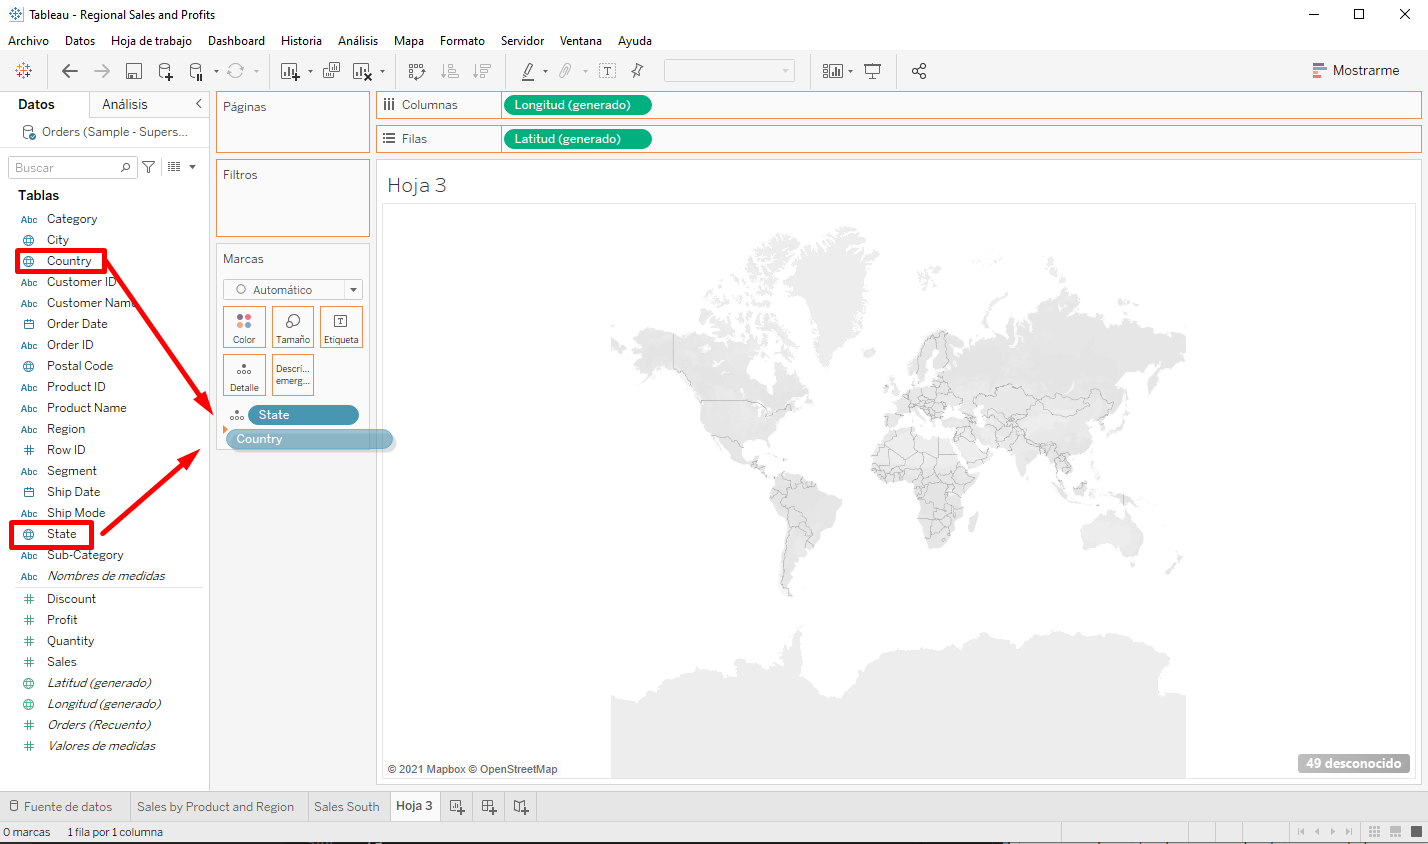
\includegraphics[width=15cm]{./img/img33.png}
        \end{center}
        \item Arrastre \textit{\textbf{Region}} a la estantería \textit{\textbf{Filters}}.
        \begin{center}
            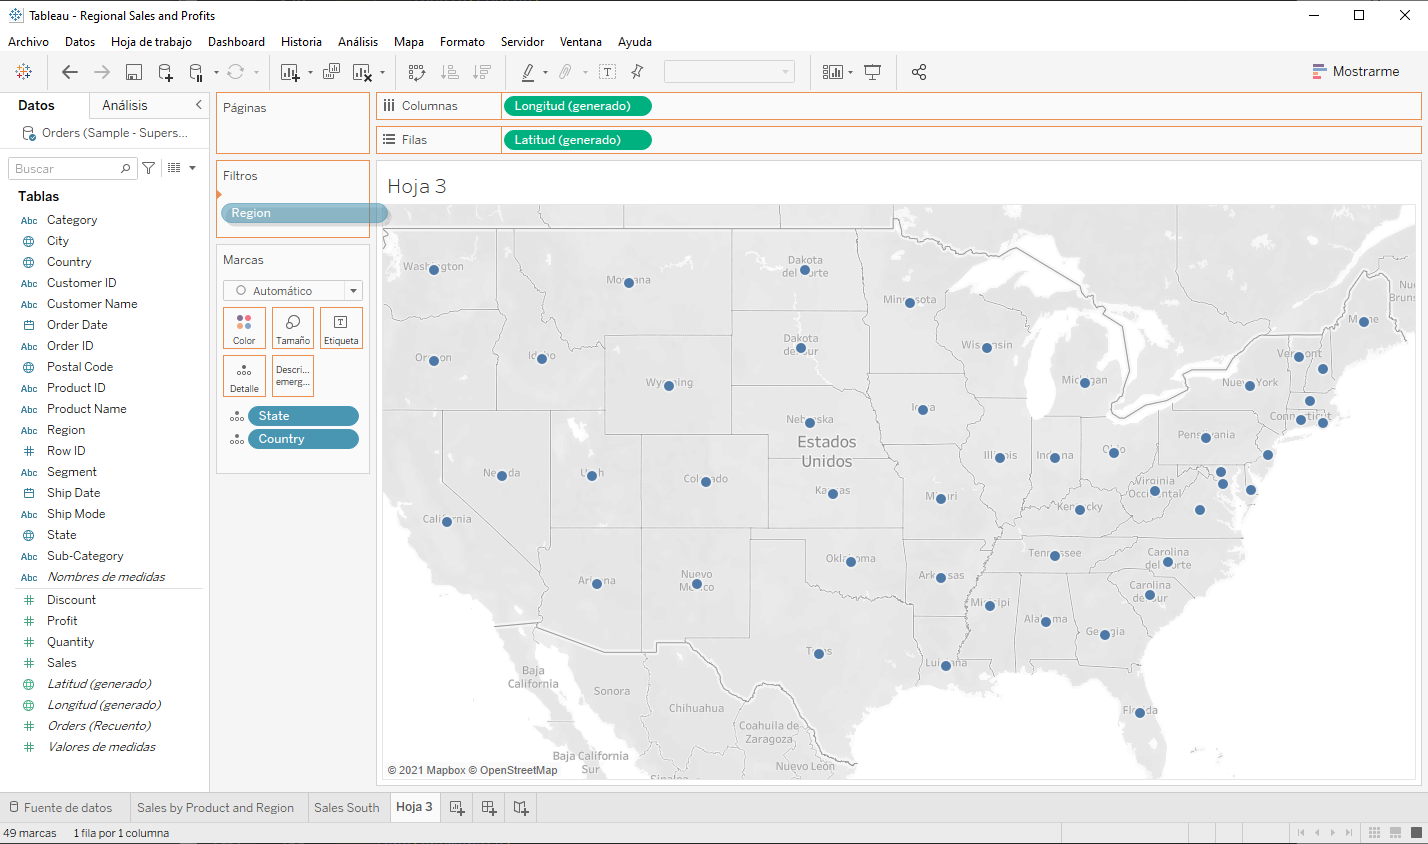
\includegraphics[width=15cm]{./img/img34.png}
        \end{center}
        \item Luego filtre hacia abajo \textit{\textbf{South}} solo. La vista del mapa ahora se acerca solo a la región Sur y una marca representa cada estado.
        \begin{center}
            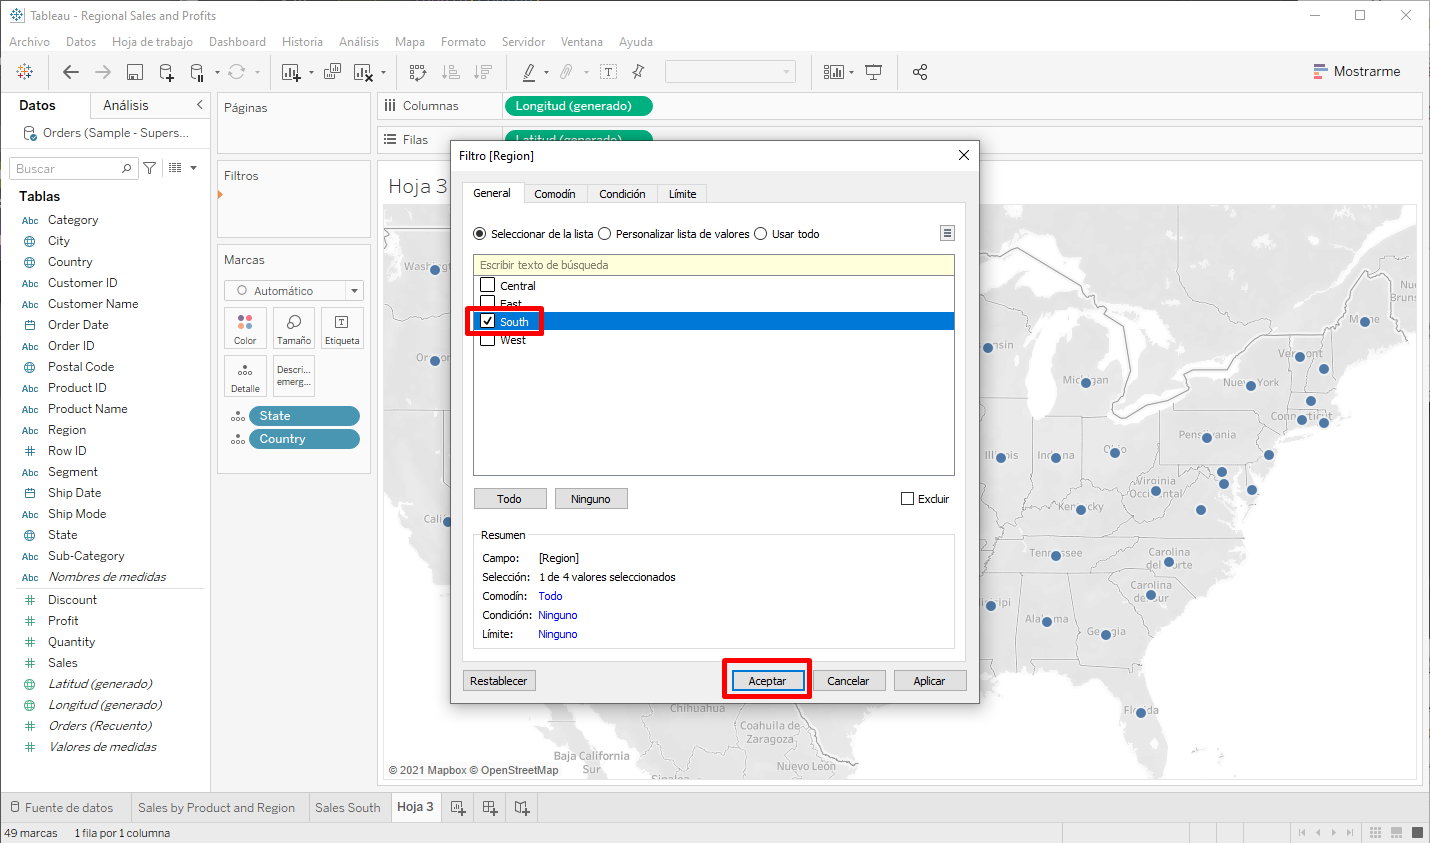
\includegraphics[width=15cm]{./img/img35.png}
        \end{center}
        \item Arrastre la medida \textit{\textbf{Sales}} a la pestaña \textit{\textbf{Color}} de la tarjeta Marcas. Obtenemos un mapa relleno con los colores que muestra el rango de ventas en cada estado.
        \begin{center}
            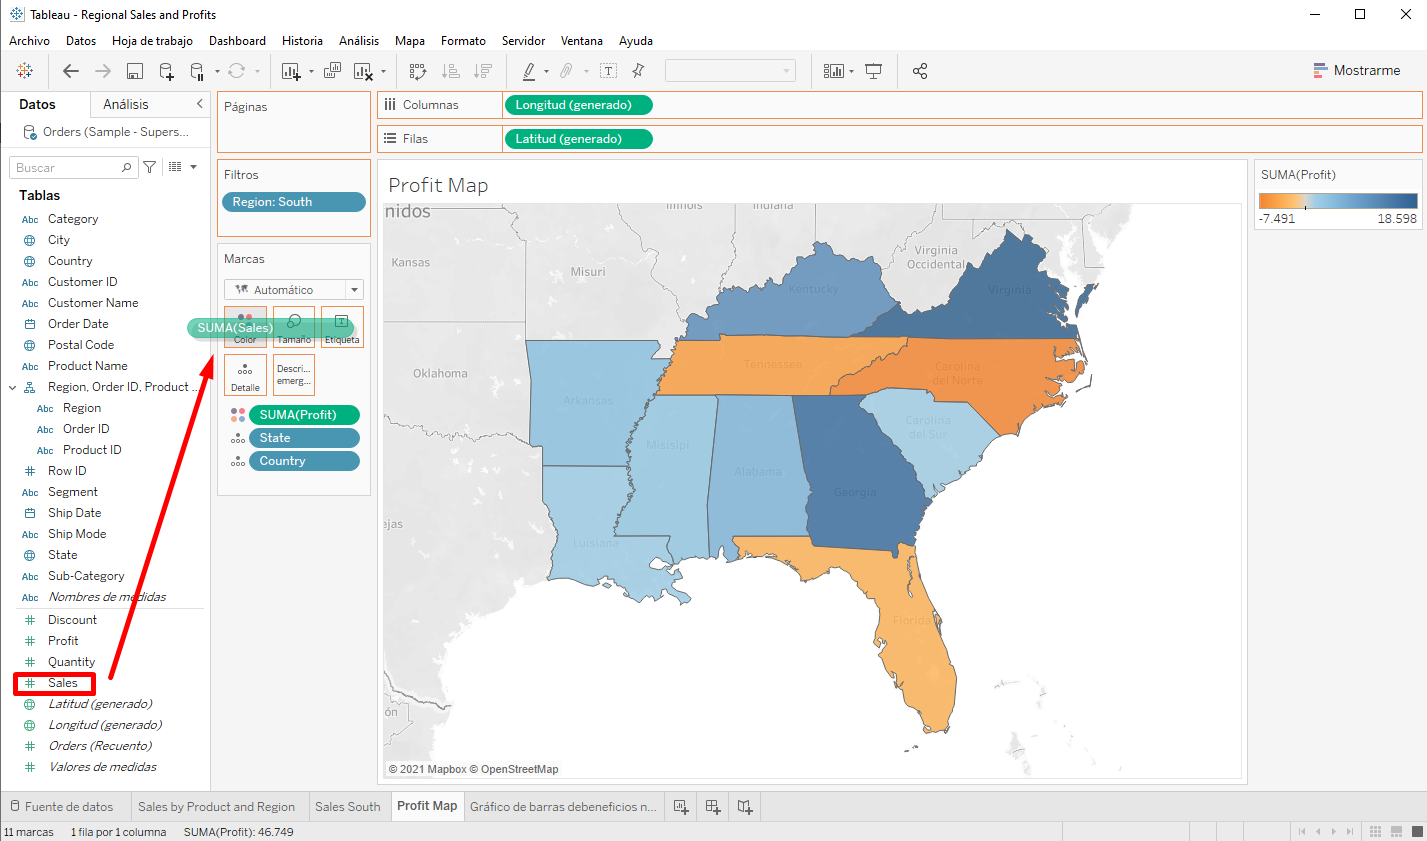
\includegraphics[width=15cm]{./img/img36.png}
        \end{center}
        \item Podemos cambiar el esquema de color haciendo clic en la tarjeta Marcas \textit{\textbf{Color}} y seleccionando \textit{\textbf{Edit Colors}}. Podemos experimentar con las paletas disponibles.
        \begin{center}
            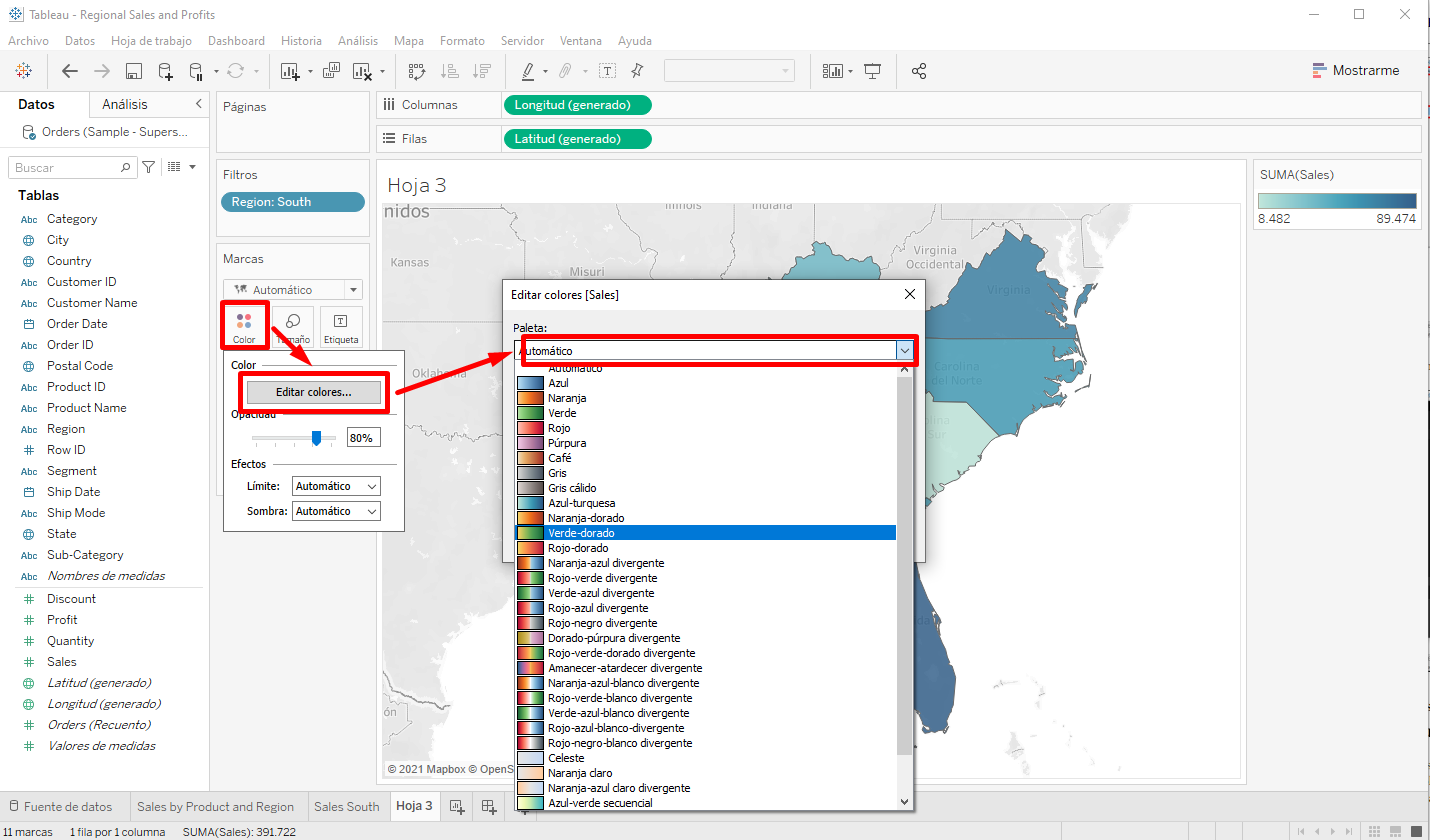
\includegraphics[width=15cm]{./img/img37.png}
        \end{center}
        \item Observamos que \textbf{Florida} se está desempeñando mejor en ventas. Si pasamos el cursor sobre \textbf{Florida}, muestra un total de 89,474 USD en ventas, en comparación con Carolina del Sur, por ejemplo, que tiene solo 8,482 USD en ventas. Evaluemos el rendimiento \textit{\textbf{Profit}} a estas alturas, ya que las ganancias son un mejor indicador que las ventas por sí solas.
        \begin{center}
            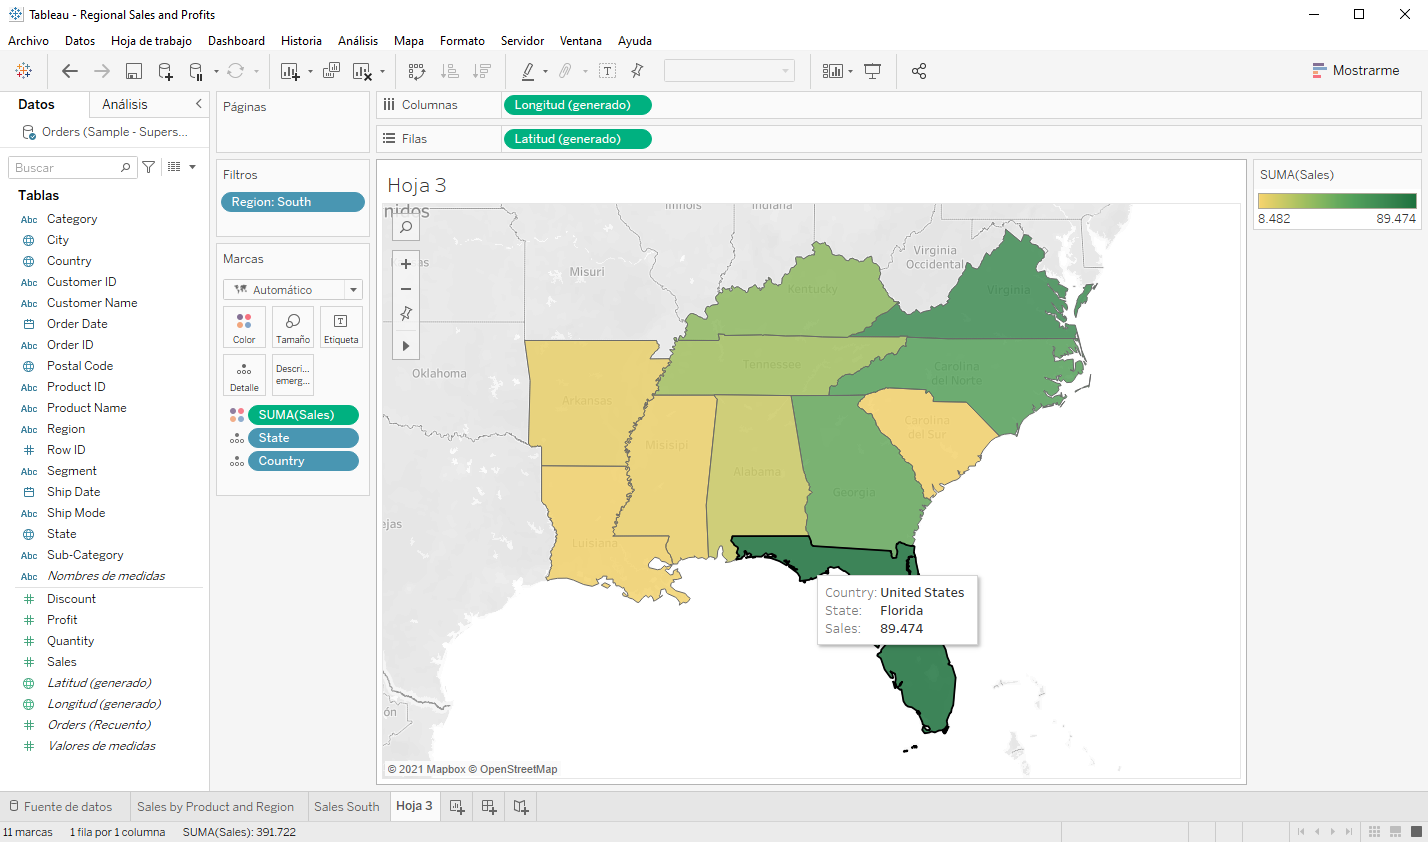
\includegraphics[width=15cm]{./img/img38.png}
        \end{center}
        \item Arrastre \textit{\textbf{Profit}} hacia \textit{\textbf{Color}} en la tarjeta Marcas. Ahora vemos que Tennessee, Carolina del Norte y Florida tienen ganancias negativas, aunque parecía que les estaba yendo bien en Ventas.
        \begin{center}
            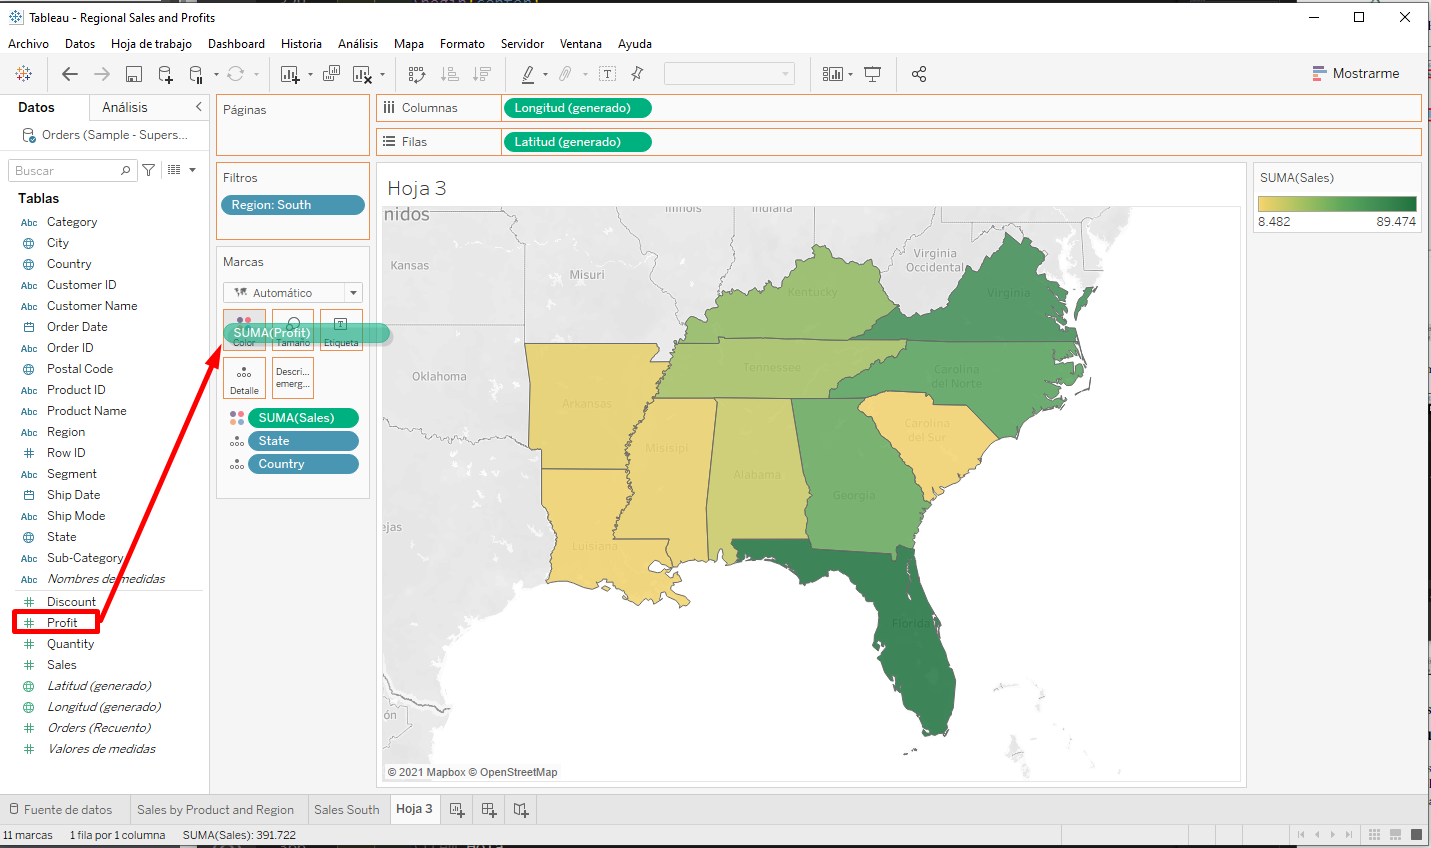
\includegraphics[width=15cm]{./img/img39.png}
        \end{center}
        \item Cambiar el nombre de la hoja como Profit Map.
        \begin{center}
            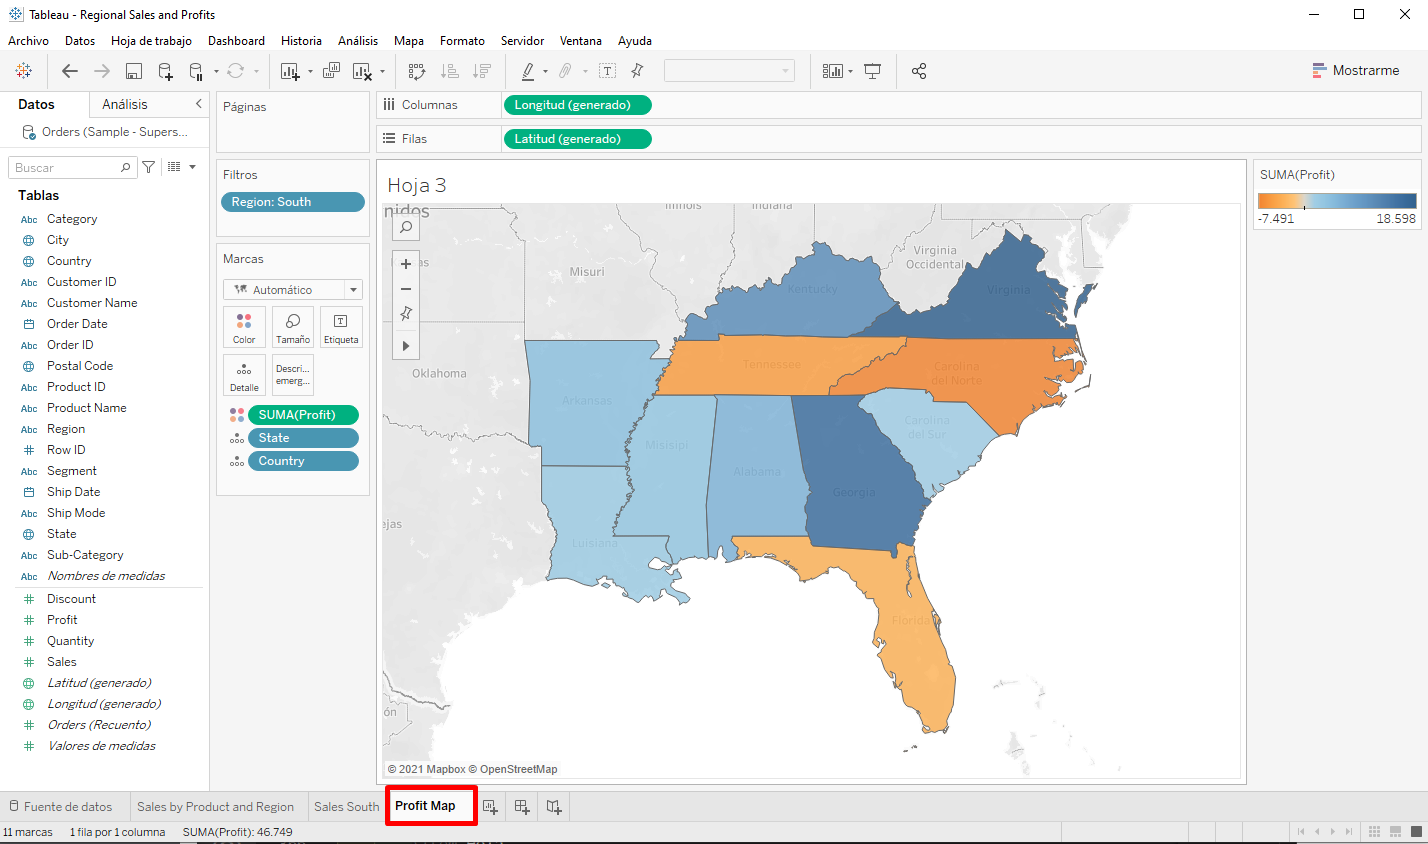
\includegraphics[width=15cm]{./img/img40.png}
        \end{center}
    \end{enumerate}t
    %--------------------------------------------------------------------------------------------------------------------------------------------------------------------------------------------------------------------------------------------------------------------------------------------------------------------------------------------------------------------------------------------------------------------------------------------------------------------------------------------------------------
    \paragraph{\Large Entrar en los detalles\\ \\}
    Los mapas nos permiten visualizar los datos de manera amplia. En el último paso, descubrimos que descubrimos que Tennessee, Carolina del Norte y Florida tienen una ganancia negativa. En esta sección dibujemos un gráfico de barras para explorar la razón de la ganancia negativa.
    \begin{enumerate}
        \item Duplique la hoja de trabajo Mapa de beneficios \textit{\textbf{Profit Map}}.
        \begin{center}
            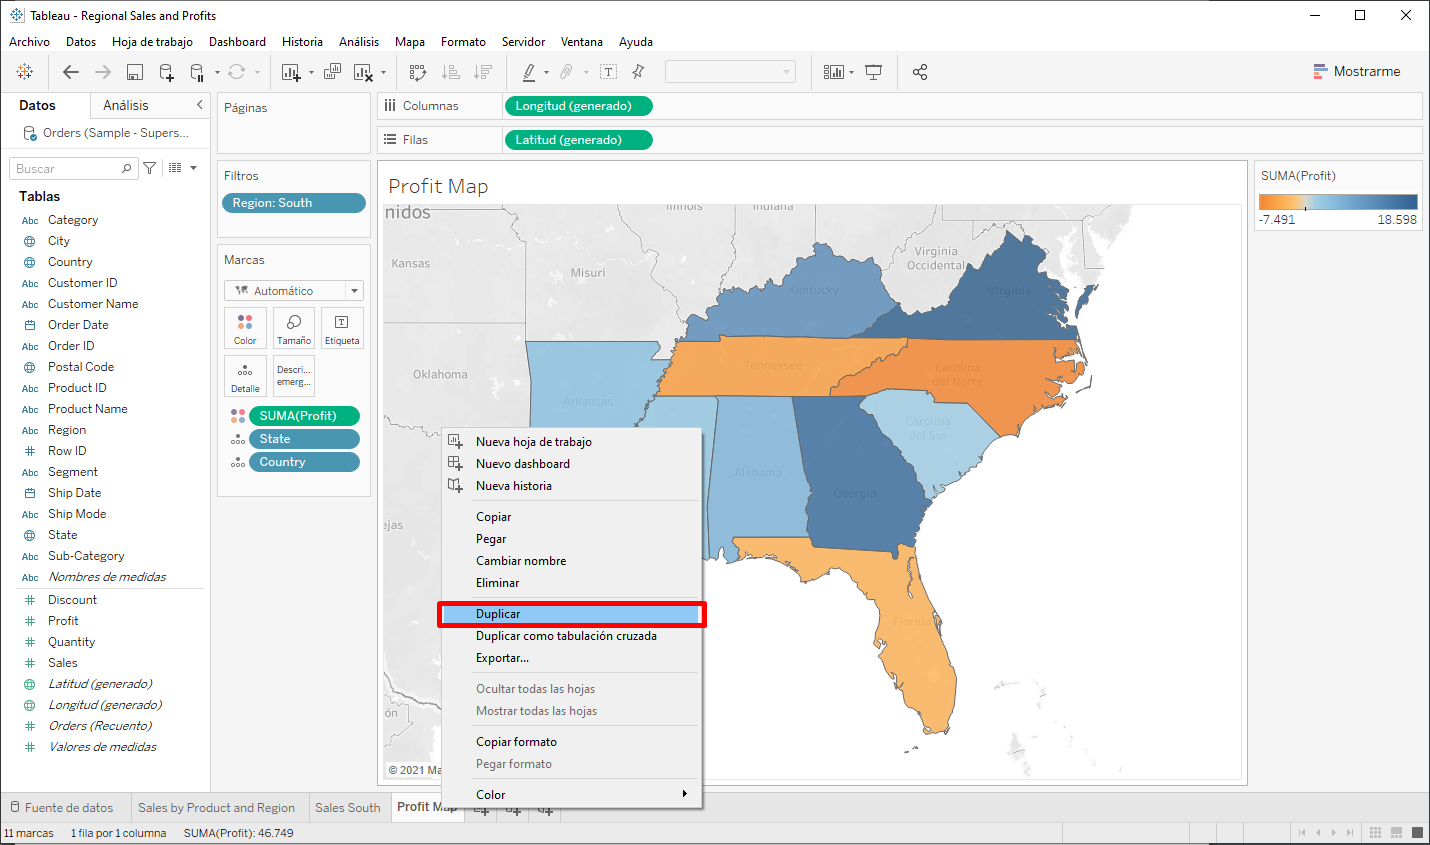
\includegraphics[width=15cm]{./img/img41.png}
        \end{center}
        \item Asígnele el nombre \textit{\textbf{Gráfico de barras de beneficios negativos}}.
        \begin{center}
            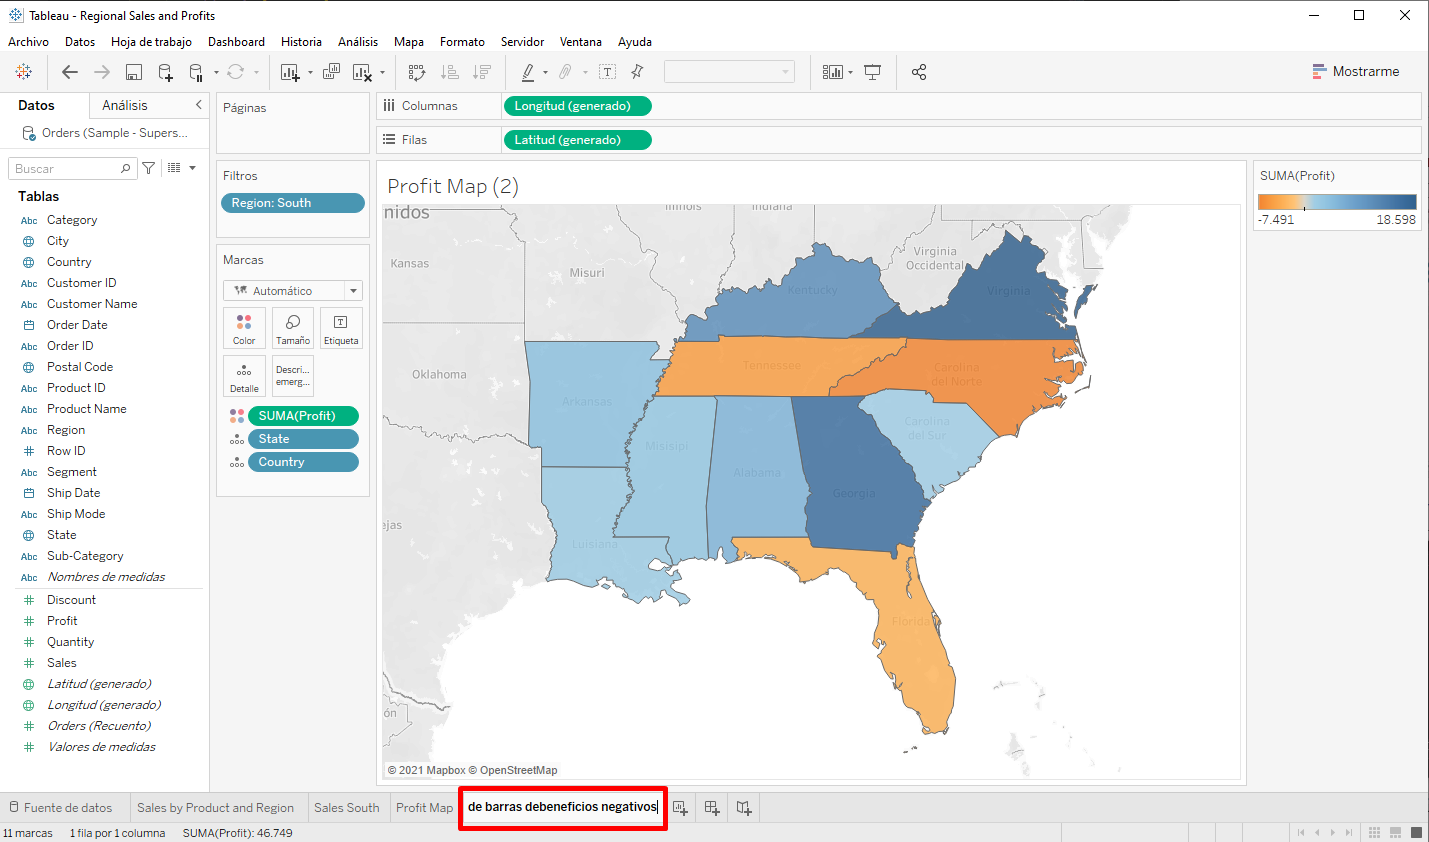
\includegraphics[width=15cm]{./img/img42.png}
        \end{center}
        \item Haga clic en \textit{\textbf{Show Me}} en la hoja de trabajo \textbf{Gráfico de barras de ganancias negativas}. \textit{\textbf{Show Me}} presenta el número de formas en que se puede trazar un gráfico entre los elementos mencionados en la hoja de trabajo.
        \begin{center}
            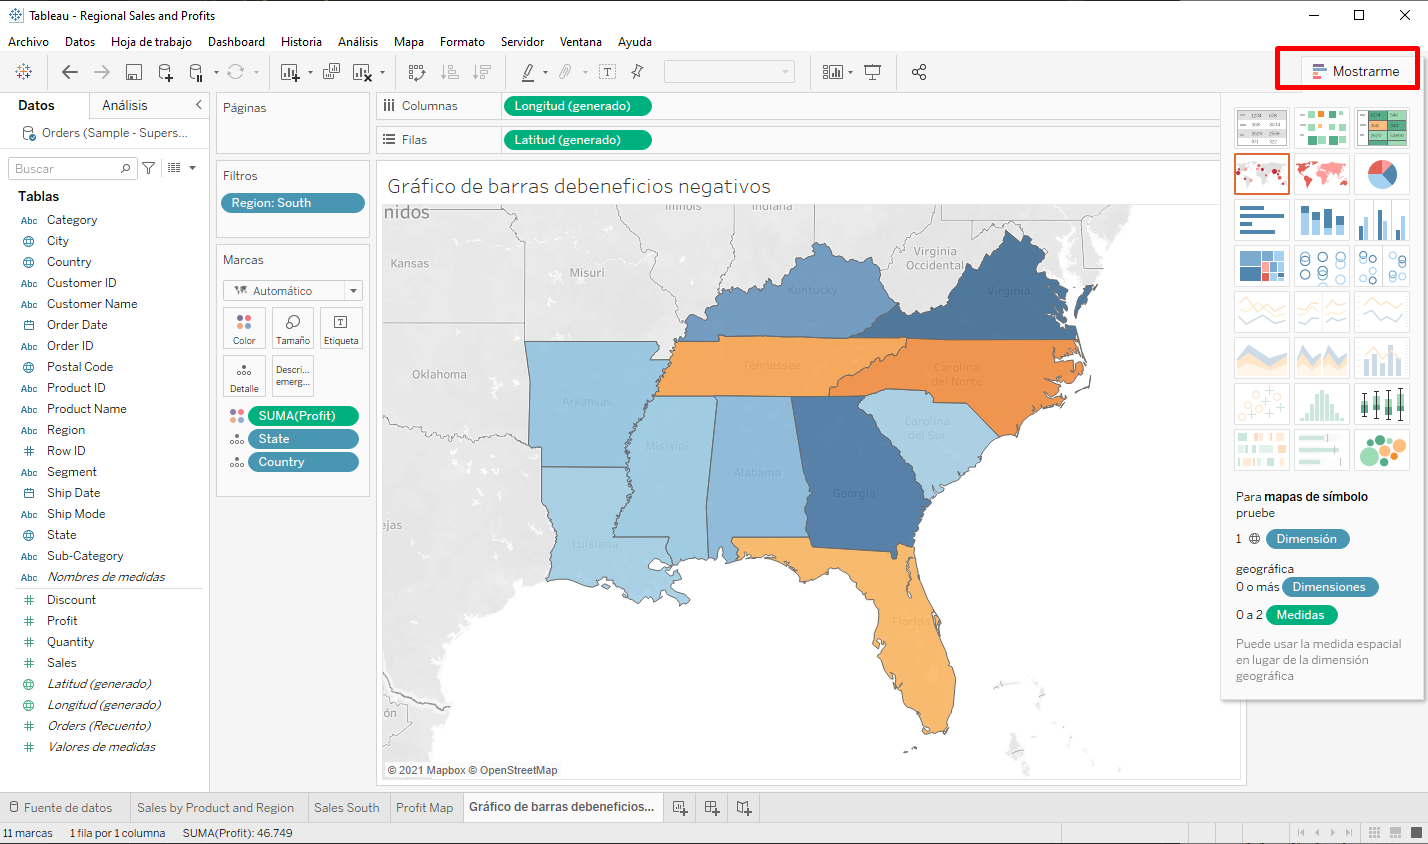
\includegraphics[width=15cm]{./img/img43.png}
        \end{center}
        \item De \textit{\textbf{Show Me}} seleccionar la opción de la barra horizontal y los cambios a vista horizontal de las barras verticales de forma instantánea.
        \begin{center}
            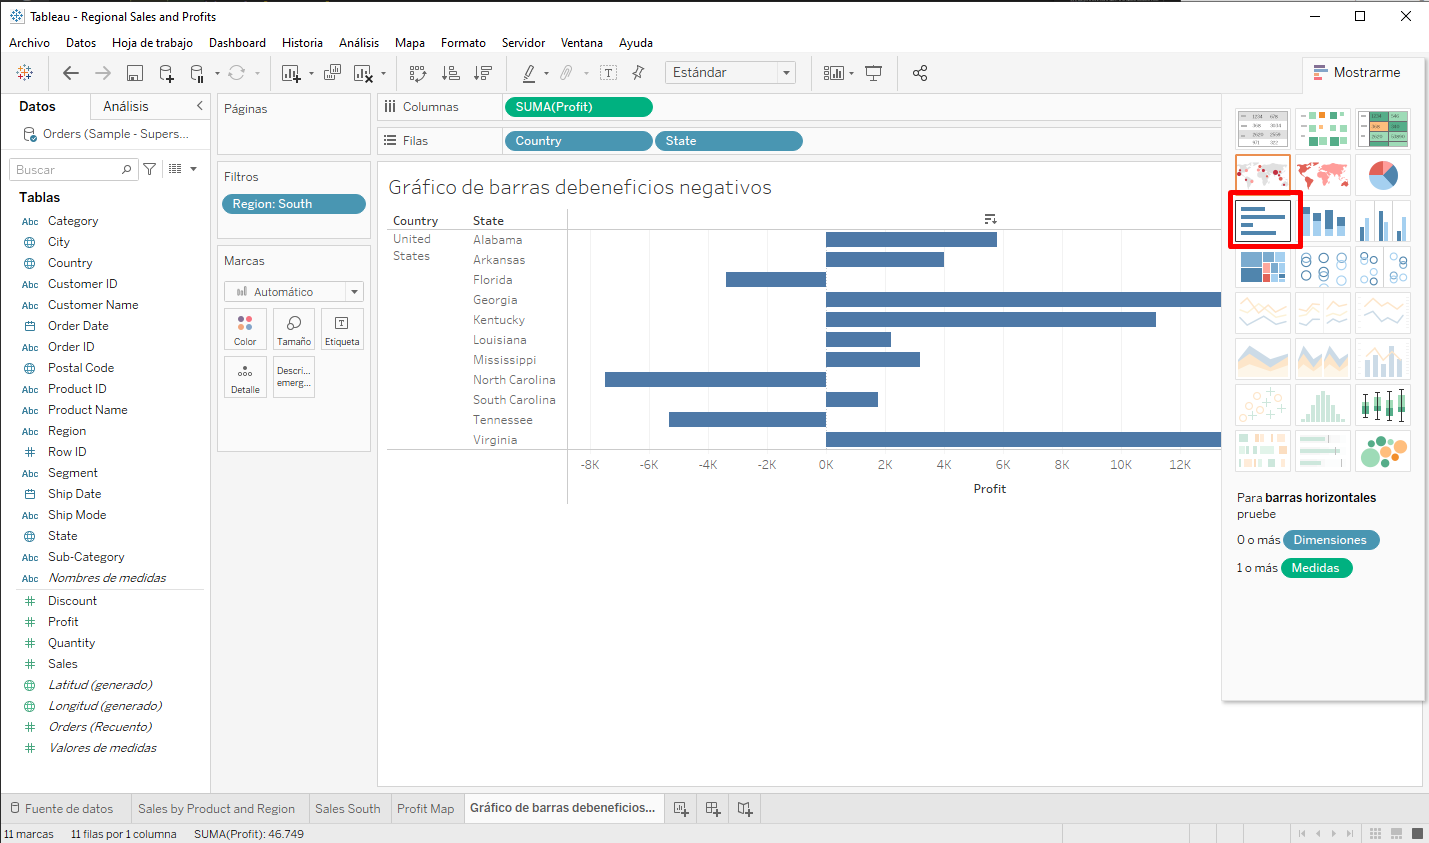
\includegraphics[width=15cm]{./img/img44.png}
        \end{center}
        \item Podemos seleccionar más de una barra a la vez simplemente haciendo clic y arrastrando el cursor sobre ellas. Queremos centrarnos únicamente en los tres estados, es decir, \textit{\textbf{Tennessee}}, \textit{\textbf{Carolina del Norte}} y \textit{\textbf{Florida}}. Por lo tanto, solo seleccionaremos las barras correspondientes.
        \begin{center}
            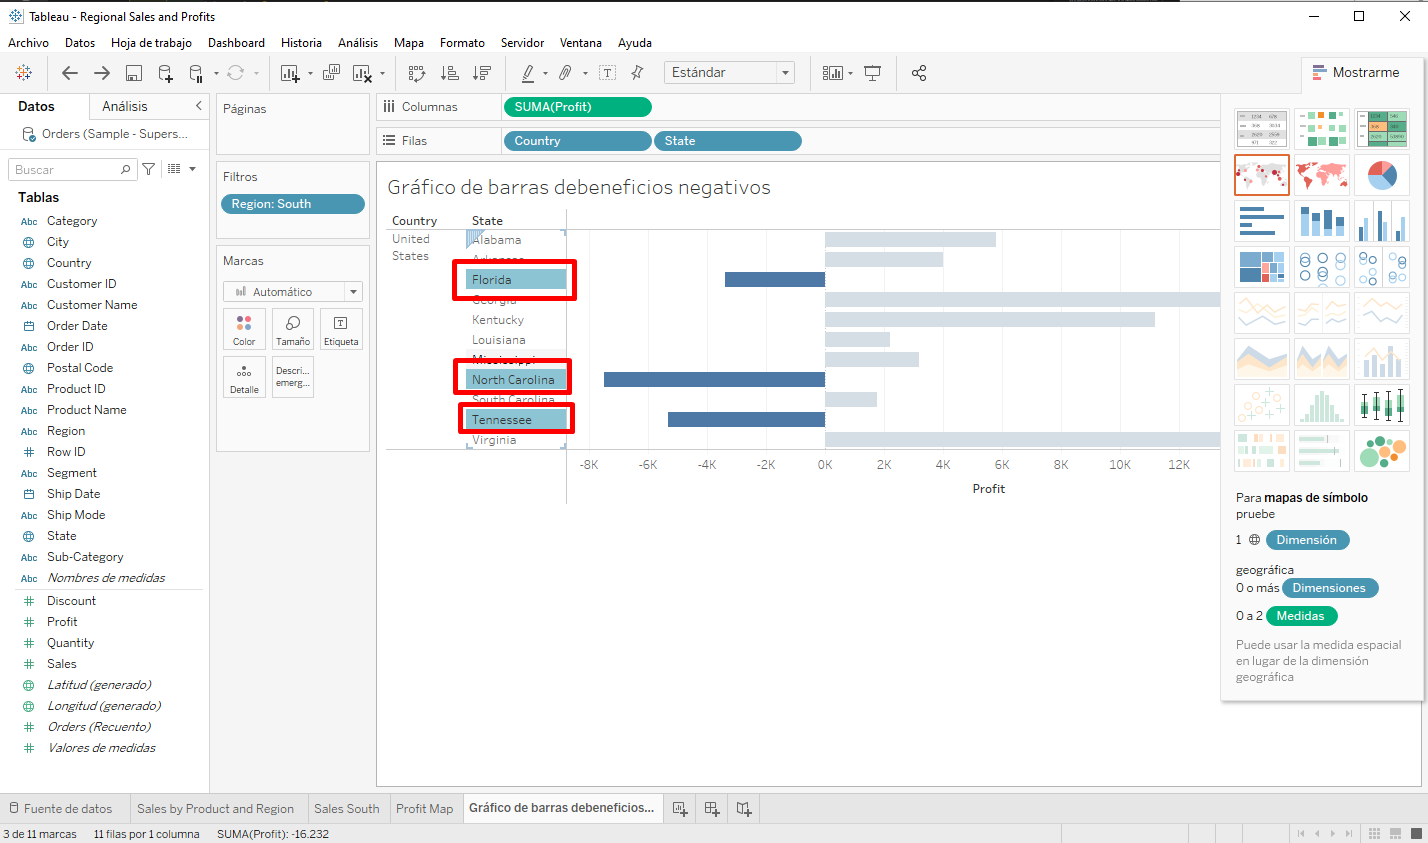
\includegraphics[width=15cm]{./img/img45.png}
        \end{center}
    \end{enumerate}
    \textbf{Creación de jerarquías:} Las jerarquías son útiles cuando queremos agrupar campos similares para poder profundizar rápidamente entre los niveles de la visualización. En el panel Datos, arrastre un campo y suéltelo directamente encima de otro campo.
    \begin{enumerate}
        \item Arrastre cualquier campo adicional a la jerarquía. Los campos también se pueden reordenar en la jerarquía simplemente arrastrándolos a una nueva posición. En la visualización actual. Crearemos las siguientes jerarquías: \textit{\textbf{Ubicación}}, \textit{\textbf{Pedido}} y \textit{\textbf{Producto}}.
        \begin{center}
            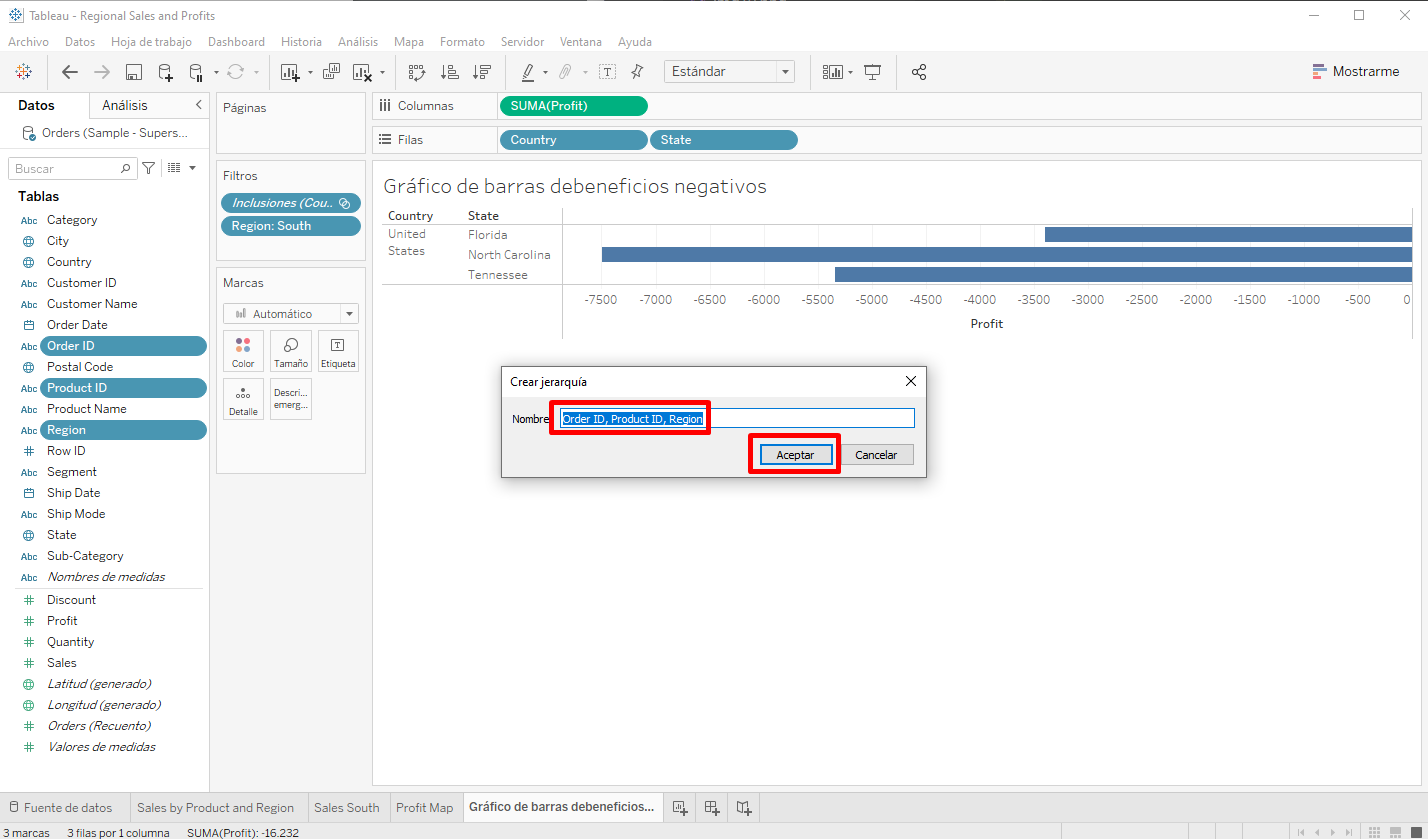
\includegraphics[width=15cm]{./img/img46.png}
        \end{center}
        \item En el estante de filas, haga clic en el icono con forma de más nivel en el campo \textit{\textbf{State}} para desglosar el \textit{\textbf{City}}.      
        \begin{center}
            \includegraphics[width=15cm]{./img/img47.png}
        \end{center}
        \item Eso es una gran cantidad de datos. Podemos usar \textit{\textbf{N-Filter}} para filtrar y revelar los que tienen un desempeño más débil. Para eso, arrastre \textit{\textbf{City}} desde el panel \textit{\textbf{Data}} al estante Filtros.
        \begin{center}
            \includegraphics[width=15cm]{./img/img48.png}
        \end{center}
        \item Haga clic en el campo Por y luego haga clic en el \textit{\textbf{Top}} menú desplegable y seleccione \textit{\textbf{Bottom}} para revelar los resultados más bajos . Escriba 5 en el cuadro de texto para mostrar los 5 mejores resultados en el conjunto de datos.
        \begin{center}
            \includegraphics[width=15cm]{./img/img49.png}
        \end{center}
        \item Ahora vemos que Jacksonville y Miami, Florida; Burlington, Carolina del Norte; y Knoxville y Memphis, Tennessee, son las ciudades con peor desempeño en términos de ganancias. Hay otra marca en la vista, Jacksonville, Carolina del Norte, que no pertenece aquí ya que tiene ventas rentables. Esto significa que hay un problema en el filtro que aplicamos. Aceptaremos la ayuda de Tableau Order of Operations.
        \begin{center}
            \includegraphics[width=15cm]{./img/img50.png}
        \end{center}
        \item En el estante Filtros, haga clic con el botón derecho en el conjunto Inclusiones (país, estado) y seleccione \textit{\textbf{Add to Context}}.
        \begin{center}
            \includegraphics[width=15cm]{./img/img51.png}
        \end{center}
        \item Encontramos que ahora Concord (Carolina del Norte) aparece a la vista mientras Miami (Florida) han desaparecido. Esto tiene sentido ahora.
        \begin{center}
            \includegraphics[width=15cm]{./img/img52.png}
        \end{center}
        \item Pero \textit{\textbf{Jacksonville}} (\textit{\textbf{Carolina del Norte}}) todavía está presente, lo cual es incorrecto. En el estante Filas, haga clic en el icono con forma de más en la \textit{\textbf{City}} pestaña para profundizar en el nivel de Código postal.
        \begin{center}
            \includegraphics[width=15cm]{./img/img53.png}
        \end{center}
        \item Haga clic con el botón derecho en el código postal de Jacksonville, NC, 28540, y luego seleccione \textit{\textbf{Exclude}} para excluir \textbf{Jacksonville} manualmente.
        \begin{center}
            \includegraphics[width=15cm]{./img/img54.png}
        \end{center}
        \item Arrastre Código postal del estante Filas.
        \begin{center}
            \includegraphics[width=15cm]{./img/img55.png}
        \end{center}
        \item Esta es la vista final.
        \begin{center}
            \includegraphics[width=15cm]{./img/img56.png}
        \end{center}
    \end{enumerate}
    %--------------------------------------------------------------------------------------------------------------------------------------------------------------------------------------------------------------------------------------------------------------------------------------------------------------------------------------------------------------------------------------------------------------------------------------------------------------------------------------------------------------
    \paragraph{\Large Resultados clave\\ \\}
    Centrémonos ahora solo en las entidades que generan pérdidas, es decir, los Productos y también identifiquemos las ubicaciones donde se venden dichos productos.
    \begin{enumerate}
        \item Arrastre \textit{\textbf{Sub-Category}} a las Filas para profundizar más.
        \begin{center}
            \includegraphics[width=15cm]{./img/img57.png}
        \end{center}
        \item Del mismo modo, arrastre \textit{\textbf{Profit}} hacia \textit{\textbf{Color}} en la tarjeta Marcas. Esto nos permite detectar rápidamente productos con beneficios negativos..
        \begin{center}
            \includegraphics[width=15cm]{./img/img58.png}
        \end{center}
        \item Haga clic derecho en \textit{\textbf{Order Date}} y seleccione \textit{\textbf{Show Filter}}.
        \begin{center}
            \includegraphics[width=15cm]{./img/img59.png}
        \end{center}
        \item Parece que las máquinas, las tablas y las carpetas funcionan mal. ¿Entonces, qué debemos hacer? ¿Una solución sería detener la venta de estos productos en Jacksonville, Concord, Burlington, Knoxville y Memphis? Verifiquemos si nuestra decisión es correcta.
        \begin{center}
            \includegraphics[width=15cm]{./img/img60.png}
        \end{center}
        \item Regresemos a la pestaña \textit{\textbf{Profit Map}} de la hoja creada anteriormente.
        \begin{center}
            \includegraphics[width=15cm]{./img/img61.png}
        \end{center}
        \item Ahora, haga clic en el campo \textit{\textbf{Sub-Category}} para seleccionar la opción \textit{\textbf{Show Filter}}.
        \begin{center}
            \includegraphics[width=15cm]{./img/img62.png}
        \end{center}
        \item Arrastre \textit{\textbf{Profit}} desde abajo Measures hasta la tarjeta \textit{\textbf{Label}} Marcas.
        \begin{center}
            \includegraphics[width=15cm]{./img/img63.png}
        \end{center}
        \item Nuevamente, haga clic en \textit{\textbf{Order Date}} y seleccione \textit{\textbf{Show Filter}}.
        \begin{center}
            \includegraphics[width=15cm]{./img/img64.png}
        \end{center}
        \item Del filtro, eliminemos los elementos que creemos que contribuyen al beneficio negativo. Por lo tanto, desmarque las  casillas frente a \textbf{Carpetas}, \textbf{Máquinas} y \textbf{Tablas}, respectivamente.
        \begin{center}
            \includegraphics[width=15cm]{./img/img65.png}
        \end{center}
        \item Ahora solo nos quedan las entidades lucrativas. Esto muestra que las entidades como los aglutinantes, las máquinas y las tablas en realidad estaban causando pérdidas en algunas áreas y teníamos razón en nuestros hallazgos.
        \begin{center}
            \includegraphics[width=15cm]{./img/img66.png}
        \end{center}
    \end{enumerate}
    %%%%%%%%%%%%%%%%%%%%%%%%%%%%%%%%%%%%%%%%%%%%%%%%%%%%%%%%%%%%%%%%%%%%%%%%%%%%%%%%%%%%%%%%%%%%%%%%%%%%%%%%%%%%%%%%%%%%%%%%%%%%%%%%%%%%%%%%%%%%%%%%%%%%%%%%%%%%%%%%%%%%%%%%%%%%%%%%%%%%%%%%%%%%%%%%%%%%%%%%%%%%%%%%%%%%%%%%%%%%%%%%%%%%%%%%%%%%%%%%%%%%%%%%%%%%%%%%%%%%%%%%%%%%%%%%%%%%%%%%%%%%%%%%%%%%%%%%%%%%%%%%%%%%%%%%%%%%%%%%%%%%%%%%%%%%%%%%%%%%%%%%%%%%%%%%%%%%%%%%%%%%%%%%%%%%%%%%%%%%%%%%%%%%%%%%%%%%%%%%%%%%%%%%%%%%%%%%%%%%%%%%%%%%%%%%%%%%%%%%%%%%%%%%%%%%%%%%%%%%%%%%%%%%%%%%%%%%%%%%%%%%%%%%%%%%%%%
    \subsection{Tablero}
    Un tablero es una colección de varias vistas, lo que permite comparar una variedad de datos simultáneamente.
    \paragraph{\Large Crear un tablero}
    \begin{enumerate}
        \item Haga clic en el botón \textit{\textbf{New dashboard}}.
        \begin{center}
            \includegraphics[width=15cm]{./img/img67.png}
        \end{center}
        \item Arrastra \textit{\textbf{Sales in the South}} al tablero vacío.
        \begin{center}
            \includegraphics[width=15cm]{./img/img68.png}
        \end{center}
        \item Arrastre \textit{\textbf{Profit Map}} al tablero y suéltelo encima de Ventas en la vista Sur.
        \begin{center}
            \includegraphics[width=15cm]{./img/img69.png}
        \end{center}
        \item Ambas vistas se pueden ver a la vez. Para poder presentar los datos de manera que otros puedan entenderlos, podemos organizar el tablero a nuestro gusto.
        \begin{center}
            \includegraphics[width=15cm]{./img/img70.png}
        \end{center}
        \item En la hoja de trabajo \textit{\textbf{Sales South}} en la vista del tablero, haga clic debajo de \textit{\textbf{Region}} y borre \textit{\textbf{Show Header}}.
        \begin{center}
            \includegraphics[width=15cm]{./img/img71.png}
        \end{center}
        \item Repita el mismo proceso para todos los demás encabezados. Esto ayuda a enfatizar solo lo que se necesita y oculta la información no tan importante.
        \begin{center}
            \includegraphics[width=15cm]{./img/img72.png}
        \end{center}
        \item En el \textit{\textbf{Profit Map}}, Ocultar el título también.
        \begin{center}
            \includegraphics[width=15cm]{./img/img73.png}
        \end{center}
        \item Realizar los mismos pasos para el mapa \textit{\textbf{Sales South}}.
        \begin{center}
            \includegraphics[width=15cm]{./img/img74.png}
        \end{center}
        \item Podemos ver que la tarjeta \textit{\textbf{Sub-Category}} de filtro y \textit{\textbf{Year of Order Date}} se han repetido en el lado derecho.
        \begin{center}
            \includegraphics[width=15cm]{./img/img75.png}
        \end{center}
        \item Eliminemos los extras simplemente tachándolos.
        \begin{center}
            \includegraphics[width=15cm]{./img/img76.png}
        \end{center}
        \item Finalmente, haga clic en el \textit{\textbf{Year of Order Date}}. Aparece una flecha desplegable y seleccione la opción de \textit{\textbf{Single Value (Slider)}}.
        \begin{center}
            \includegraphics[width=15cm]{./img/img77.png}
        \end{center}
        \item Ahora deja que la magia se desarrolle. Experimente eligiendo diferentes años en el control deslizante y las Ventas también variarán en consecuencia.
        \begin{center}
            \includegraphics[width=15cm]{./img/img78.png}
        \end{center}
        \item Arrastre el \textit{\textbf{SUM(Profit)}} filtro a la parte inferior del panel debajo de Ventas en el sur.
        \begin{center}
            \includegraphics[width=15cm]{./img/img79.png}
        \end{center}
        \item De esa manera se obtiene una mejor vista.
        \begin{center}
            \includegraphics[width=15cm]{./img/img80.png}
        \end{center}
    \end{enumerate}
    %--------------------------------------------------------------------------------------------------------------------------------------------------------------------------------------------------------------------------------------------------------------------------------------------------------------------------------------------------------------------------------------------------------------------------------------------------------------------------------------------------------------
    \paragraph{\Large Añadiendo interactividad\\ \\}
    Para que el panel de control sea más interactivo, como ver qué subcategorías son rentables en qué estados, es necesario realizar algunos cambios.
    \begin{enumerate}
        \item Comencemos con el \textit{\textbf{Profit Map}}. Al hacer clic en el mapa, \textit{\textbf{Use as filter}} aparece un icono en la parte superior derecha. Haz click en eso.
        \begin{center}
            \includegraphics[width=15cm]{./img/img81.png}
        \end{center}
        \item Si seleccionamos cualquier mapa, las Ventas correspondientes a ese estado se resaltarán en el mapa \textit{\textbf{SalesSouth}}.
        \begin{center}
            \includegraphics[width=15cm]{./img/img82.png}
        \end{center}
        \item Para el \textit{\textbf{Year of Order Date}}, haga clic en la opción desplegable y vaya a \textit{\textbf{Apply to Worksheets $>$ Selected Worksheets}}.
        \begin{center}
            \includegraphics[width=15cm]{./img/img83.png}
        \end{center}
        \item Se abre un cuadro de diálogo. Seleccione la opción \textit{\textbf{All}} seguida de \textit{\textbf{OK}}. ¿Qué hace esta opción? Aplica filtros a todas las hojas de trabajo que tienen la misma fuente de datos.
        \begin{center}
            \includegraphics[width=15cm]{./img/img84.png}
        \end{center}
        \item Explore y experimente. En la visualización a continuación, podemos filtrar el mapa \textit{\textbf{Sales South}} para ver los productos que se venden solo en Carolina del Norte. Luego, podemos explorar fácilmente las ganancias anuales.
        \begin{center}
            \includegraphics[width=15cm]{./img/img85.png}
        \end{center}
        \item Cambie el nombre del panel a \textit{\textbf{Regional Sales and Profit}}.
        \begin{center}
            \includegraphics[width=15cm]{./img/img86.png}
        \end{center}
    \end{enumerate}
    Por lo tanto, la venta de máquinas en Carolina del Norte no reportó beneficios a la empresa.
    %%%%%%%%%%%%%%%%%%%%%%%%%%%%%%%%%%%%%%%%%%%%%%%%%%%%%%%%%%%%%%%%%%%%%%%%%%%%%%%%%%%%%%%%%%%%%%%%%%%%%%%%%%%%%%%%%%%%%%%%%%%%%%%%%%%%%%%%%%%%%%%%%%%%%%%%%%%%%%%%%%%%%%%%%%%%%%%%%%%%%%%%%%%%%%%%%%%%%%%%%%%%%%%%%%%%%%%%%%%%%%%%%%%%%%%%%%%%%%%%%%%%%%%%%%%%%%%%%%%%%%%%%%%%%%%%%%%%%%%%%%%%%%%%%%%%%%%%%%%%%%%%%%%%%%%%%%%%%%%%%%%%%%%%%%%%%%%%%%%%%%%%%%%%%%%%%%%%%%%%%%%%%%%%%%%%%%%%%%%%%%%%%%%%%%%%%%%%%%%%%%%%%%%%%%%%%%%%%%%%%%%%%%%%%%%%%%%%%%%%%%%%%%%%%%%%%%%%%%%%%%%%%%%%%%%%%%%%%%%%%%%%%%%%%%%%%%%
    \subsection{Historia}
    Un tablero es una característica interesante, pero tableau también nos ofrece mostrar nuestros resultados en el modo de presentación en forma de historias sobre las que hablaremos en esta sección.
    \paragraph{\Large Construyendo una historia\\ \\}
    \begin{enumerate}
        \item Haga clic en el botón \textit{\textbf{New story}}.
        \begin{center}
            \includegraphics[width=15cm]{./img/img87.png}
        \end{center}
        \item Desde el panel Historia a la izquierda, arrastre la hoja de trabajo (creada anteriormente) \textit{\textbf{Sales in the South}} a la vista.
        \begin{center}
            \includegraphics[width=15cm]{./img/img88.png}
        \end{center}
        \item Edite el texto en el cuadro gris sobre la hoja de trabajo. Este es el título. Nómbrelo como \textit{\textbf{Sales and profit by year}}.
        \begin{center}
            \includegraphics[width=15cm]{./img/img89.png}
        \end{center}
        \item Las historias son bastante específicas. Aquí contaremos una historia sobre la venta de máquinas en Carolina del Norte. En el panel Historia, haga clic en \textit{\textbf{Duplicate}} para duplicar el primer título, o incluso puede crear uno nuevo.
        \begin{center}
            \includegraphics[width=15cm]{./img/img90.png}
        \end{center}
        \item En el \textit{\textbf{Sub-Category}}, \textit{\textbf{select}} solo filtro \textit{\textbf{Machines}}. Esto ayuda a medir las ventas y los beneficios de las máquinas por año.
        \begin{center}
            \includegraphics[width=15cm]{./img/img91.png}
        \end{center}
        \item Cambie el nombre del título a \textit{\textbf{Machine sales and profit by year}}.
        \begin{center}
            \includegraphics[width=15cm]{./img/img92.png}
        \end{center}
    \end{enumerate}
    %--------------------------------------------------------------------------------------------------------------------------------------------------------------------------------------------------------------------------------------------------------------------------------------------------------------------------------------------------------------------------------------------------------------------------------------------------------------------------------------------------------------
    \paragraph{\Large Hacer una conclusión\\ \\}
    Está claro que las máquinas en Carolina del Norte están provocando pérdidas de beneficios. Sin embargo, esto no se puede demostrar observando las ganancias y las ventas en su conjunto. Para ello, necesitamos Beneficio regional.
    \begin{enumerate}
        \item En el panel Historia, seleccione \textit{\textbf{Blank}}. Arrastre el panel ya creado \textit{\textbf{Regional Sales and Profit}} al lienzo.
        \begin{center}
            \includegraphics[width=15cm]{./img/img93.png}
        \end{center}
        \item Subtitúlelo como \textit{\textbf{Low performing items in the South}}.
        \begin{center}
            \includegraphics[width=15cm]{./img/img94.png}
        \end{center}
        \item Seleccione \textit{\textbf{Duplicate}} para crear otro punto de la historia con el panel de ganancias regionales.
        \begin{center}
            \includegraphics[width=15cm]{./img/img95.png}
        \end{center}
        \item Seleccione Carolina del Norte en el gráfico de barras, ya que estamos interesados en mostrar más al respecto.
        \begin{center}
            \includegraphics[width=15cm]{./img/img96.png}
        \end{center}
        \item Seleccione Todos los años.
        \begin{center}
            \includegraphics[width=15cm]{./img/img97.png}
        \end{center}
        \item Agregar un título para mayor claridad, como, \textit{\textbf{Profit in NC : 2014-2017}}.
        \begin{center}
            \includegraphics[width=15cm]{./img/img98.png}
        \end{center}
        \item Seleccione cualquier año como 2014. Agregue un título, por ejemplo, \textit{\textbf{Profit in NC: 2014}} y luego haga clic en la pestaña Duplicar.
        \begin{center}
            \includegraphics[width=15cm]{./img/img99.png}
        \end{center}
        \item Repita el mismo paso para todos los años restantes.
        \begin{center}
            \includegraphics[width=15cm]{./img/img100.png}
        \end{center}
        \item Haz clic en el modo de presentación y deja que se \textit{\textbf{story}} desarrolle.
        \begin{center}
            \includegraphics[width=15cm]{./img/img101.png}
        \end{center}
    \end{enumerate}
    Ahora tenemos una idea acerca de qué productos se introdujeron en el mercado de Carolina del Norte, cuándo y cómo funcionaron. No solo hemos identificado una forma de abordar las ganancias negativas, sino que también hemos logrado respaldarlas con datos. Ésta es la ventaja de Story en Tableau.
    %%%%%%%%%%%%%%%%%%%%%%%%%%%%%%%%%%%%%%%%%%%%%%%%%%%%%%%%%%%%%%%%%%%%%%%%%%%%%%%%%%%%%%%%%%%%%%%%%%%%%%%%%%%%%%%%%%%%%%%%%%%%%%%%%%%%%%%%%%%%%%%%%%%%%%%%%%%%%%%%%%%%%%%%%%%%%%%%%%%%%%%%%%%%%%%%%%%%%%%%%%%%%%%%%%%%%%%%%%%%%%%%%%%%%%%%%%%%%%%%%%%%%%%%%%%%%%%%%%%%%%%%%%%%%%%%%%%%%%%%%%%%%%%%%%%%%%%%%%%%%%%%%%%%%%%%%%%%%%%%%%%%%%%%%%%%%%%%%%%%%%%%%%%%%%%%%%%%%%%%%%%%%%%%%%%%%%%%%%%%%%%%%%%%%%%%%%%%%%%%%%%%%%%%%%%%%%%%%%%%%%%%%%%%%%%%%%%%%%%%%%%%%%%%%%%%%%%%%%%%%%%%%%%%%%%%%%%%%%%%%%%%%%%%%%%%%%%
    \newpage
    \section{CONCLUSIONES}
    \begin{itemize}
        \item Tableau es una herramienta de análisis y visualización de datos que se utiliza ampliamente en la industria actual. Muchas empresas incluso lo consideran indispensable para el trabajo relacionado con la ciencia de datos. La facilidad de uso de Tableau proviene del hecho de que tiene una interfaz de arrastrar y soltar. Esta función ayuda a realizar tareas como clasificar, comparar y analizar, de manera muy fácil y rápida.
        \item Tableau también es compatible con múltiples fuentes, incluidos Excel, SQL Server y repositorios de datos basados en la nube, lo que lo convierte en una excelente opción para los científicos de datos.
    \end{itemize}
    %%%%%%%%%%%%%%%%%%%%%%%%%%%%%%%%%%%%%%%%%%%%%%%%%%%%%%%%%%%%%%%%%%%%%%%%%%%%%%%%%%%%%%%%%%%%%%%%%%%%%%%%%%%%%%%%%%%%%%%%%%%%%%%%%%%%%%%%%%%%%%%%%%%%%%%%%%%%%%%%%%%%%%%%%%%%%%%%%%%%%%%%%%%%%%%%%%%%%%%%%%%%%%%%%%%%%%%%%%%%%%%%%%%%%%%%%%%%%%%%%%%%%%%%%%%%%%%%%%%%%%%%%%%%%%%%%%%%%%%%%%%%%%%%%%%%%%%%%%%%%%%%%%%%%%%%%%%%%%%%%%%%%%%%%%%%%%%%%%%%%%%%%%%%%%%%%%%%%%%%%%%%%%%%%%%%%%%%%%%%%%%%%%%%%%%%%%%%%%%%%%%%%%%%%%%%%%%%%%%%%%%%%%%%%%%%%%%%%%%%%%%%%%%%%%%%%%%%%%%%%%%%%%%%%%%%%%%%%%%%%%%%%%%%%%%%%%%
    \newpage
    \section{WEBGRAFIA}
    \begin{itemize}
        \item Datacamp. (2018). Data Visualisation with Tableau.\\
        Recuperado de \textcolor{azul}{\url{https://www.datacamp.com/community/tutorials/data-visualisation-tableau}}
        \item Tableau. (2021). Ayuda de Tableau.\\
        Recuperado de \textcolor{azul}{\url{https://www.tableau.com/es-es/support/help?_ga=2.265900495.1177855510.1601060242-2100777728.1601060242&_fsi=yk2dkG5O}}
    \end{itemize}
\end{document}